\documentclass[11pt,a4paper]{article}
\usepackage[utf8]{inputenc}
\usepackage{amsmath}
\usepackage{amsfonts}
\usepackage{amssymb}

\usepackage{todonotes}
\usepackage{todoextend}

\usepackage{color}
\usepackage{listings}
\renewcommand\lstlistingname{Code Segment}
\definecolor{dkgreen}{rgb}{0,0.6,0}
\definecolor{gray}{rgb}{0.9,0.9,0.9}
\definecolor{mauve}{rgb}{1,0.4,0}
\lstset{frame=none,
  backgroundcolor=\color{gray},
  escapeinside={\%*}{*)},
  language=R,
  aboveskip=3mm,
  belowskip=3mm,
  showstringspaces=false,
  columns=flexible,
  basicstyle={\small\ttfamily},
  numbers=left,
  numberstyle=\tiny\color{black},
  keywordstyle=\color{blue},
  commentstyle=\color{dkgreen},
  stringstyle=\color{mauve},
  breaklines=true,
  breakatwhitespace=true,
  tabsize=3,
  captionpos=b,
  xleftmargin=.25in,
  xrightmargin=.25in
}

\usepackage{multirow}

\usepackage{graphicx}
\usepackage{epstopdf} % for eps file

\usepackage{fullpage} % utilize paper space :)

\usepackage{float} % for use of [H] in figure alignment
\usepackage{subcaption} % for use of subfigures
\usepackage{tikz}

\usepackage{hyperref}
\hypersetup{
pdfborder = {0 0 0}
}



\setlength{\parindent}{0pt}
\setlength{\parskip}{0.5\baselineskip}%

\DeclareMathSizes{12}{14}{10}{10} % increase math font size

\begin{document}

\title{K-NN and Trees\\Statistical Machine Learning\\{\large\emph{Group 3}}}
\author{Nikolaj Iversen and Lukas Schwartz}
\date{June 9$^{th}$, 2015}
\maketitle

\vfill
\begin{center}
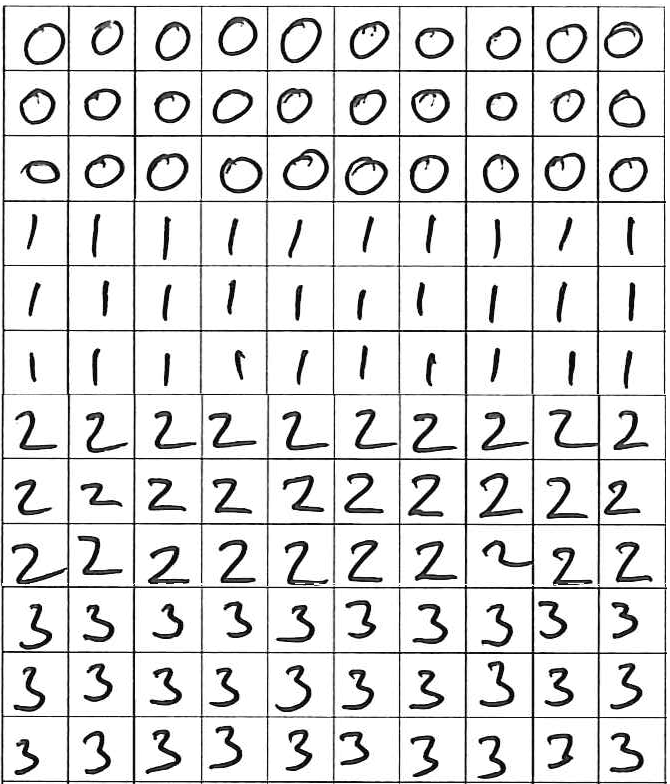
\includegraphics[width=0.7\textwidth]{graphics/digit_example}
\end{center}

\newpage


\section*{Abstract}



\section*{Acknowledgement}
This piece is written as a report by Nikolaj Iversen and Lukas Schwartz.
...


\newpage

\tableofcontents
\listoffigures
\listoftables
 \listoftodos

\newpage


\section{Introduction}
The classification of handwritten characters is used in a wide range of products to day.
Hence, this report goes in depth with how the numbers from zero to nine can be classified using machine learning algorithms.

The dataset consists of a set of handwritten characters from zero to nine.
These were constructed by the students enrolled in the course Statistical Machine learning (RM-SML-E1) of the year 2015 at the University of Southern Denmark (SDU).
The set used in this report is the 100DPI dataset.
Each number is hence stored as a $20px \times 20px$ matrix containing the handwritten character.

The methods used for classification are K-Nearest Neighbours and Decision Trees and Random Forests.
Furthermore a set of different ways to pre-process the data is explored.
Finally the two methods are compared with each at the best parameters and preprocessing settings.




\newpage

\section{Preprocessing}
\section{Introduction}
The classification of handwritten characters is used in a wide range of products to day.
Hence, this report goes in depth with how the numbers from zero to nine can be classified using machine learning algorithms.

The dataset consists of a set of handwritten characters from zero to nine.
These were constructed by the students enrolled in the course Statistical Machine learning (RM-SML-E1) of the year 2015 at the University of Southern Denmark (SDU).
The set used in this report is the 100DPI dataset.
Each number is hence stored as a $20px \times 20px$ matrix containing the handwritten character.

The methods used for classification are K-Nearest Neighbours and Decision Trees and Random Forests.
Furthermore a set of different ways to pre-process the data is explored.
Finally the two methods are compared with each at the best parameters and preprocessing settings.





\subsection{Smoothing}
The process of smoothing involves applying a kernel to an image using convolution.
Smoothing is applied to an image in order to reduce the noise in the image such that only the important features are left in the data.
A wide range of kernels can be used for smoothing, but in this report only the Gaussian kernel is considered.
Furthermore, the kernels considered here all have a sum of one, such that the brightness of the image is unchanged.

When applying a smoothing filer, the neighbouring pixels to the smoothed are added a contribution from the smoothed.
The process of smoothing hence widens the digits, as seen in figure \ref{fig:effect_smooth}, and this should give a better chance of two characters overlapping.
The danger is that too much smoothing blurs the whole image and hence remove the features in the data that is used to compare and identify the characters.

\begin{figure}[H]
\centering
	\begin{subfigure}[b]{0.2\textwidth}
	
\includegraphics[width=\textwidth]{graphics/smooth_none}
	\caption{Raw image.}
	\end{subfigure}
	\qquad
	\begin{subfigure}[b]{0.2\textwidth}
         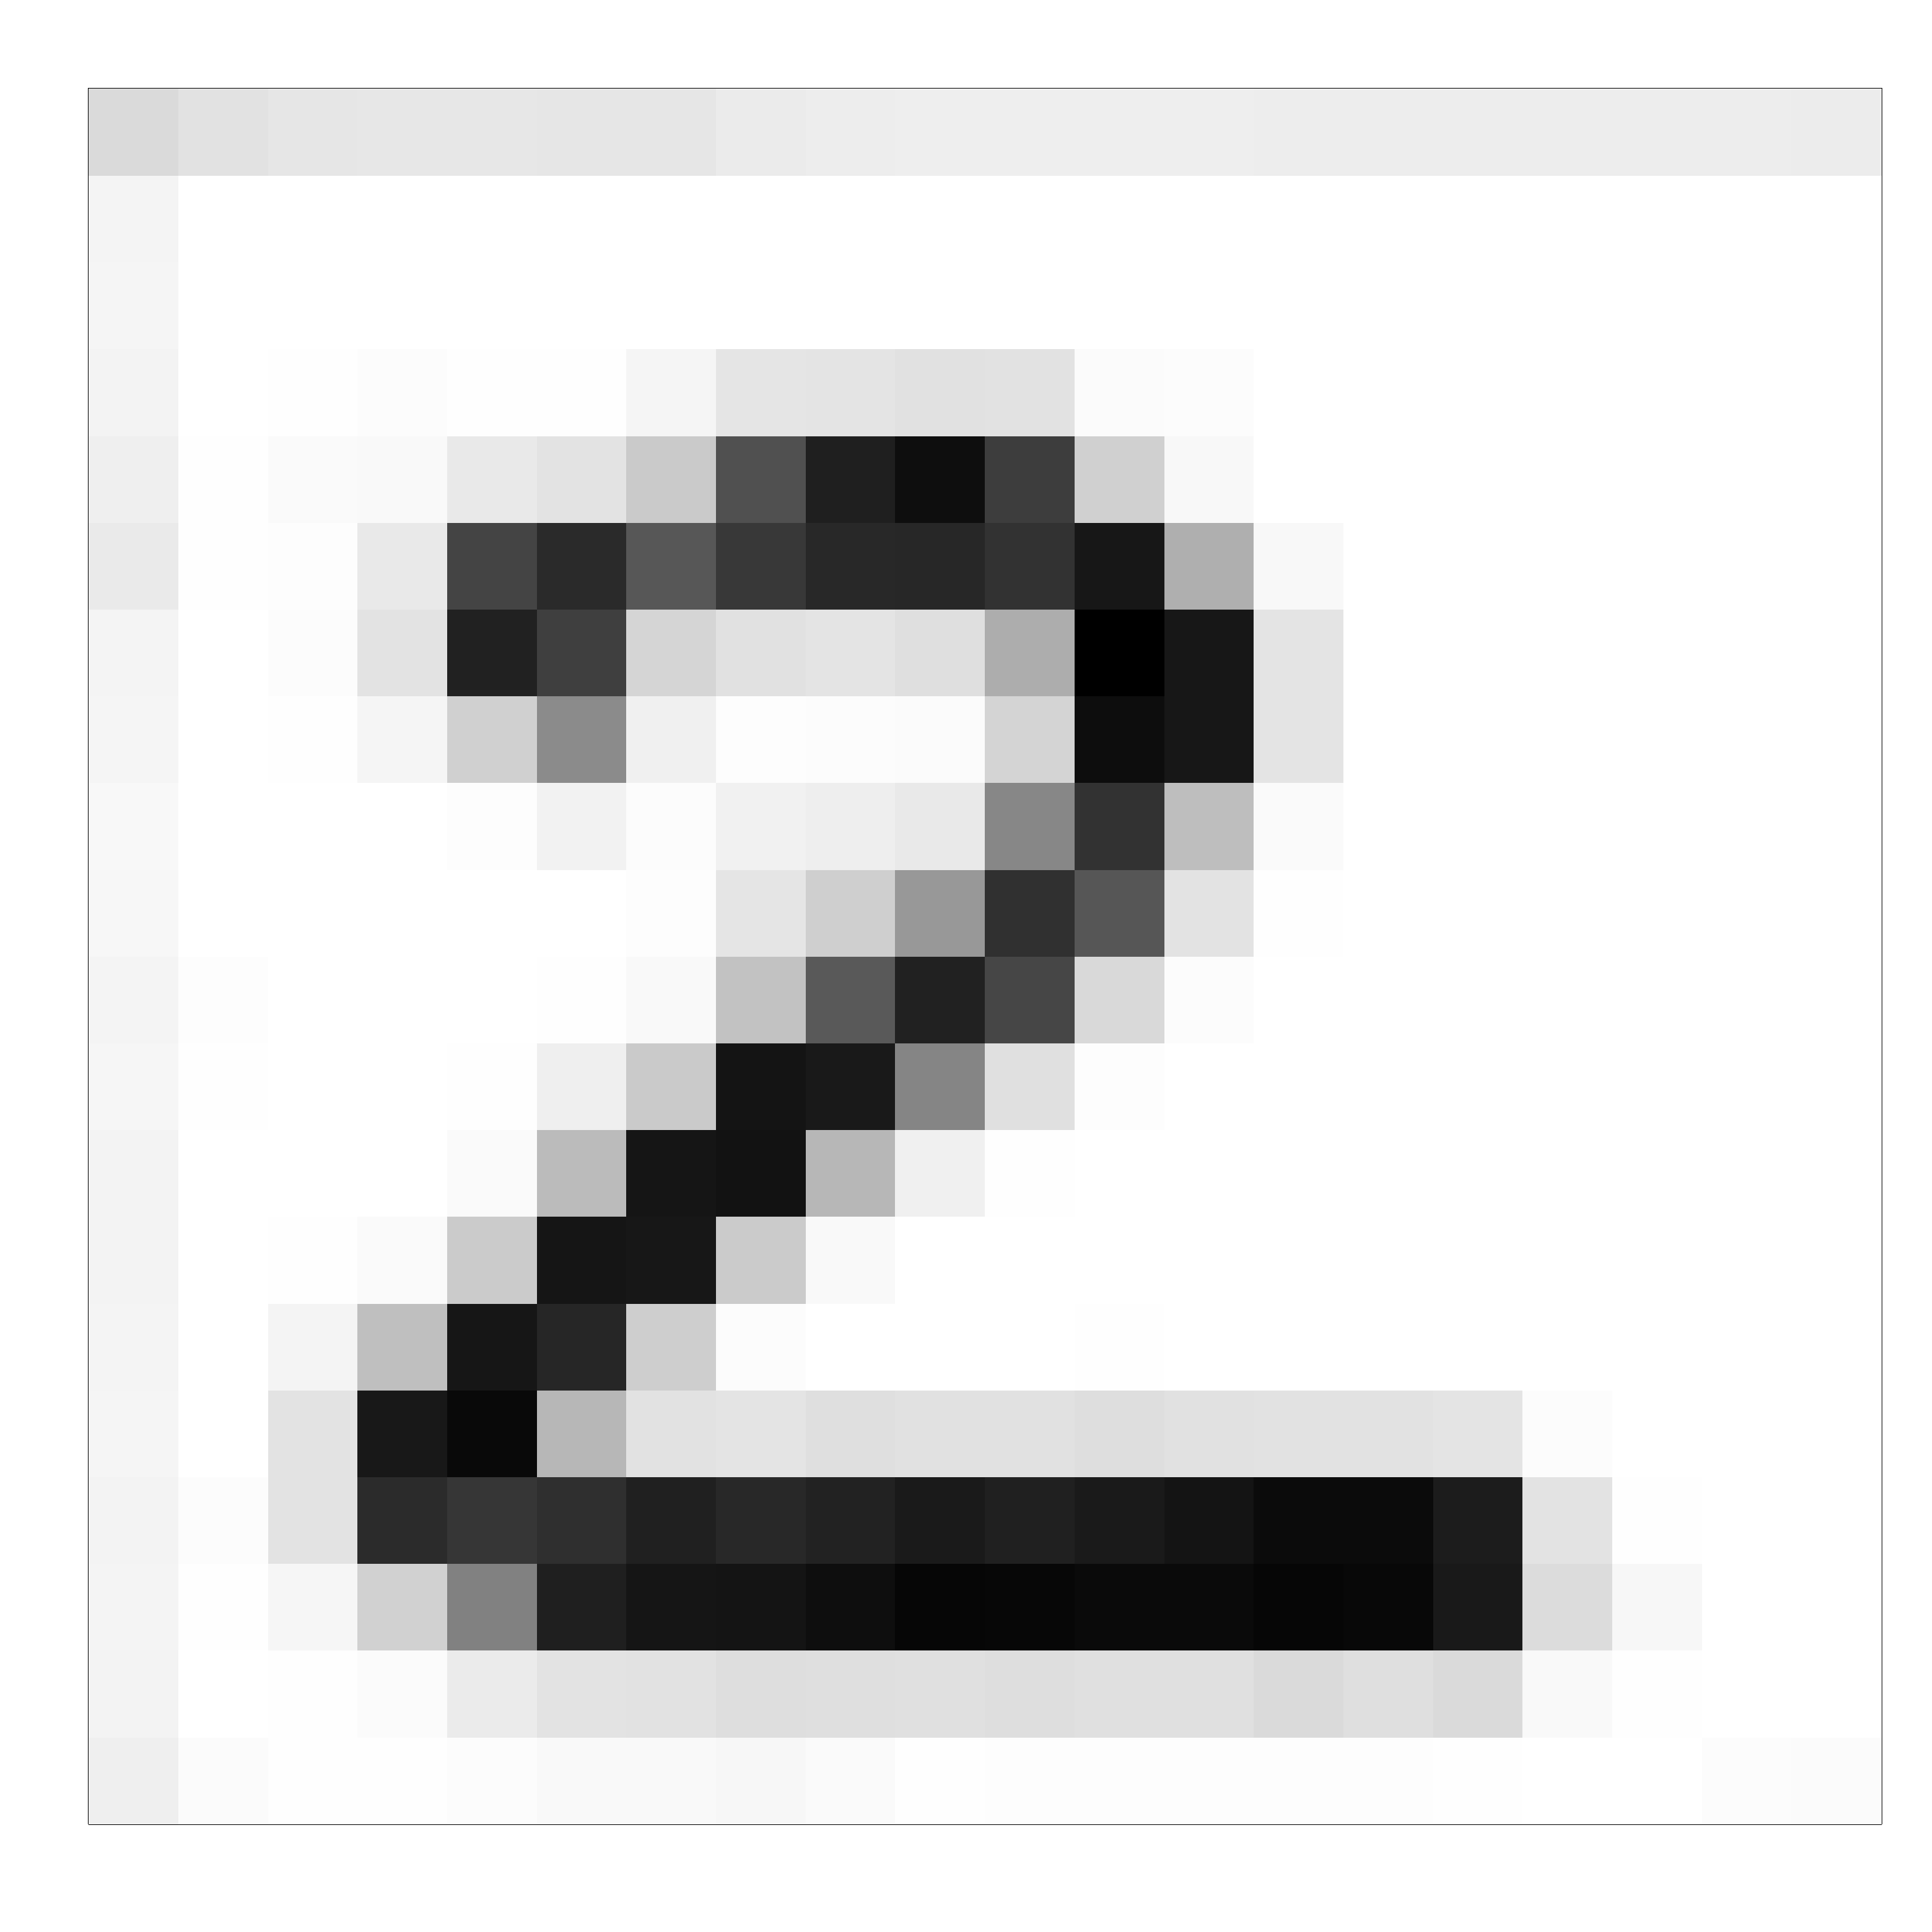
\includegraphics[width=\textwidth]{graphics/smooth_05_5}
         \caption{\(\sigma = 0.5\).}
	\end{subfigure}
	\qquad
	\begin{subfigure}[b]{0.2\textwidth}
         
\includegraphics[width=\textwidth]{graphics/smooth_1_5}
         \caption{\(\sigma = 1\).}
	\end{subfigure}
	\qquad
	\begin{subfigure}[b]{0.2\textwidth}
         
\includegraphics[width=\textwidth]{graphics/smooth_2_5}
         \caption{\(\sigma = 2\).}
	\end{subfigure}
\caption{Illustration of Gaussian smoothing. All kernels are 5x5.}
\label{fig:effect_smooth}
\end{figure}

A Gaussian distribution (also referred to as a normal distribution) is a naturally occurring distribution which is found when a random result occurs around a mean. 
The $\sigma$ signifies the deviation of the distribution. 
The 2D equation of a Gaussian distribution is shown in equation \ref{eq:gauss}. 

\begin{equation}
G(x,y) = \frac{1}{2\pi \sigma^2} e^{- \frac{x^2+y^2}{2\sigma^2}} \label{eq:gauss}
\end{equation}

Using the Gaussian filter to smooth an image will weigh the distance to the pixel.
A small $\sigma$ will make a small deviation and thus heavily weigh the center pixel.
The Gaussian filter is the one applied in figure \ref{fig:effect_smooth}.

%Applying a smoothing function can give the image an advantage when using the nearest neighbour analysis.

%The results of the filtering methods were also compared to the raw image with 100, 200 and 300 DPI.
%These results are compared with an averaging filter (avg) which takes the average of the four neighbouring pixels and a Gaussian filter (G) with different values for sigma.
%These tests were done 10 times, using cross validation, and the mean of each success rate is plotted in figure \ref{fig:smooth}. 
%Since the variance is too small to be seen in the figure the mean and variance is shown in table \ref{tb:smooth}.
%The averaging filter does not give a measurable different result from not using a filter.
%The Gaussian filter does improves the success rate for some values of sigma, but a larger $\sigma$ makes it worse.


\subsection{Z-Score}
The z-score can be used to normalizes the data.
This transforms the range of the data points measured into a standard range.
The formula to calculate the z-score is given in equation \ref{eq:zscore}.

\begin{equation}
X_{new} = \frac{X - \mu}{\sigma}
\label{eq:zscore}
\end{equation}


The z-score transforms the values into a number representing how many standard deviations the value is from the mean.

\subsection{Principle Component Analysis}
\todo[inline]{not corrected/made yet}
The Principle Components Analysis (PCA) is an tool that can be used to describe the variance in a data set.

PCA aims to reduce the number of dimension used to represent the features of the data.
This is done by finding the eigenvectors and eigenvalues to the training set and removing some of the components representing the least variance in the data set.
Thus efficiently reducing the dimensions, but still keeping the most significant knowledge about the features.

By selecting the most significant principle components (PC) the data set can be systematically reduced with minimal changes to performance.
In figure \ref{fig:variance} is the variance and accumulated variance shown for the first 20 PC. 
It is seen that the first PC is the most significant and the variance converges towards zero with more PC.

\begin{figure}[H]
\centering
\begin{subfigure}{0.70\textwidth}
\centering
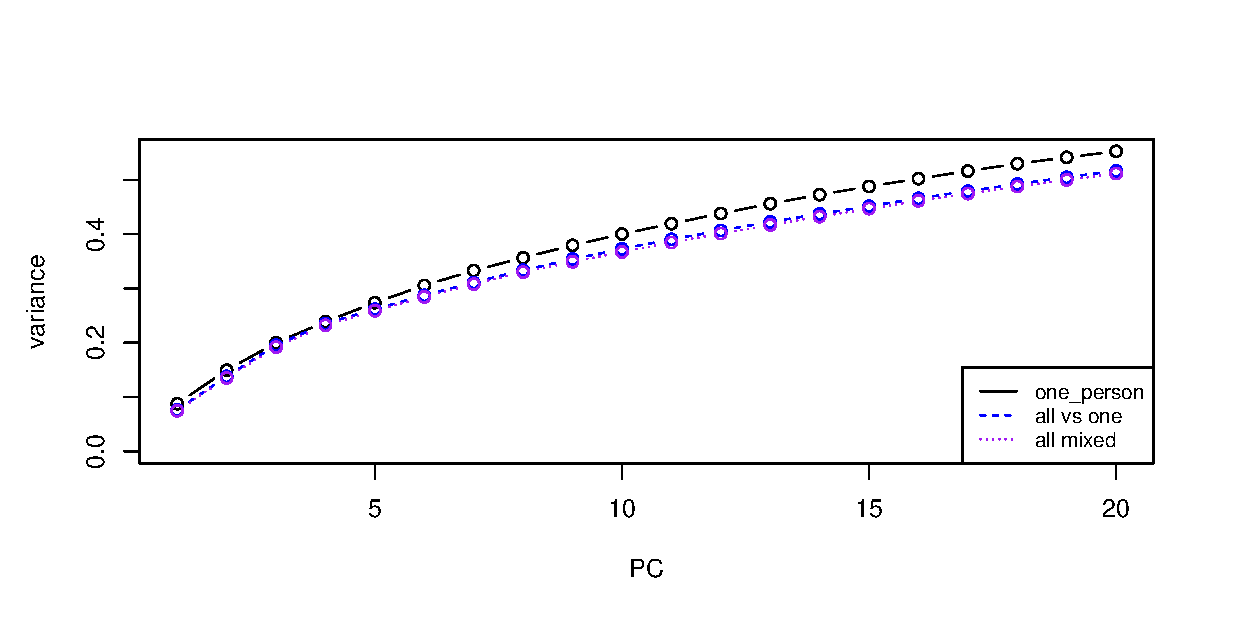
\includegraphics[width=\textwidth]{graphics/pca_acc_variance}
\caption{Accumulated variance}
\label{fig:pca_accumulated_var}
\end{subfigure}\\[-1cm]
\begin{subfigure}{0.70\textwidth}
\centering
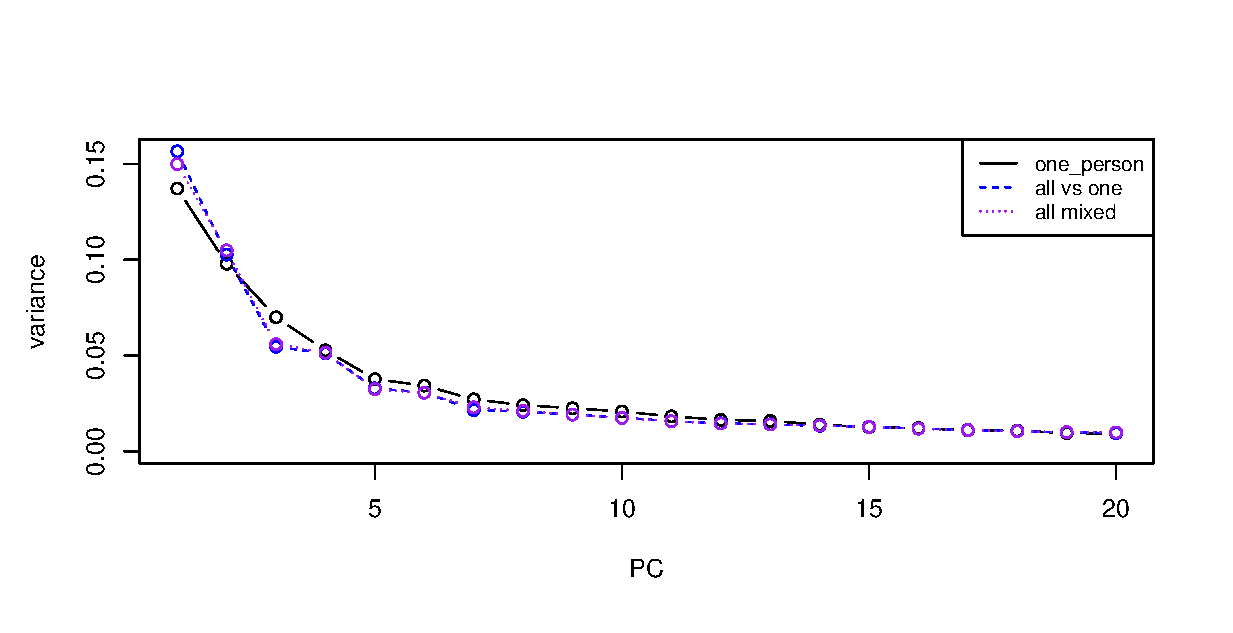
\includegraphics[width=\textwidth]{graphics/pca_variance}
\caption{Variance}
\label{fig:pca_accumulated_var}
\end{subfigure}
\caption[PCA variance]{Variance over the first 20 principle components.
The data was run on Group 3 member 2's data on 100 DPI. }
\label{fig:variance}
\end{figure}
% Figure \ref{fig:contour_KvsPCA_G3M2vsRest} shows a contour plot of how well Group 3 Member 2's  handwriting was predicted successfully for $K$ and the total variance represented of the PC's varying between one and 20 and 0.5 and 1 respectively.


Calculating with less data will result in a faster computation time.
Choosing too few PC means there is no features left to compare.
To see how the performance and the timing scales both are shown in figure \ref{fig:pca_timing_lukas} and \ref{fig:pca_timing_nikolaj}. K was chosen to be 10.
In figure \ref{fig:pca_timing_lukas} the performance seems to be the same regardless of how many PC is chosen. As long as there are more than 60 the performance will be the same.
On the test done on Group member 1 the performance is worse which means the digits are less uniform. 
Here the success rate has a peak with a low set of attributes so there must be some confusion that gets sorted out. 
Both test were run with 100 DPI. The percentage of successful predictions is also measured with the same data.
The timing was measured on the same computer so the difference should not be very large. 

\begin{figure}[H]
\centering
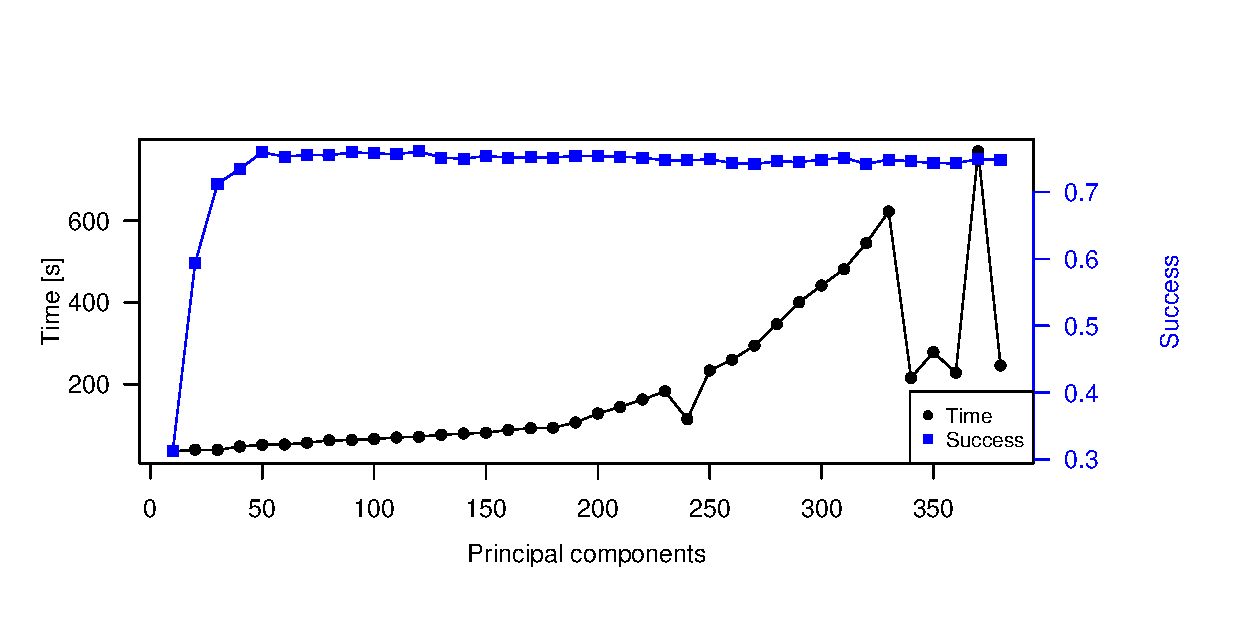
\includegraphics[width =0.8 \textwidth]{graphics/pca_timing}
\caption[Timing of PCA]{Timing of running the PCA with different principle components. 
The data was run on Group 3 member 2's data. 
}
\label{fig:pca_timing_lukas}
\end{figure}
\begin{figure}[H]
\centering
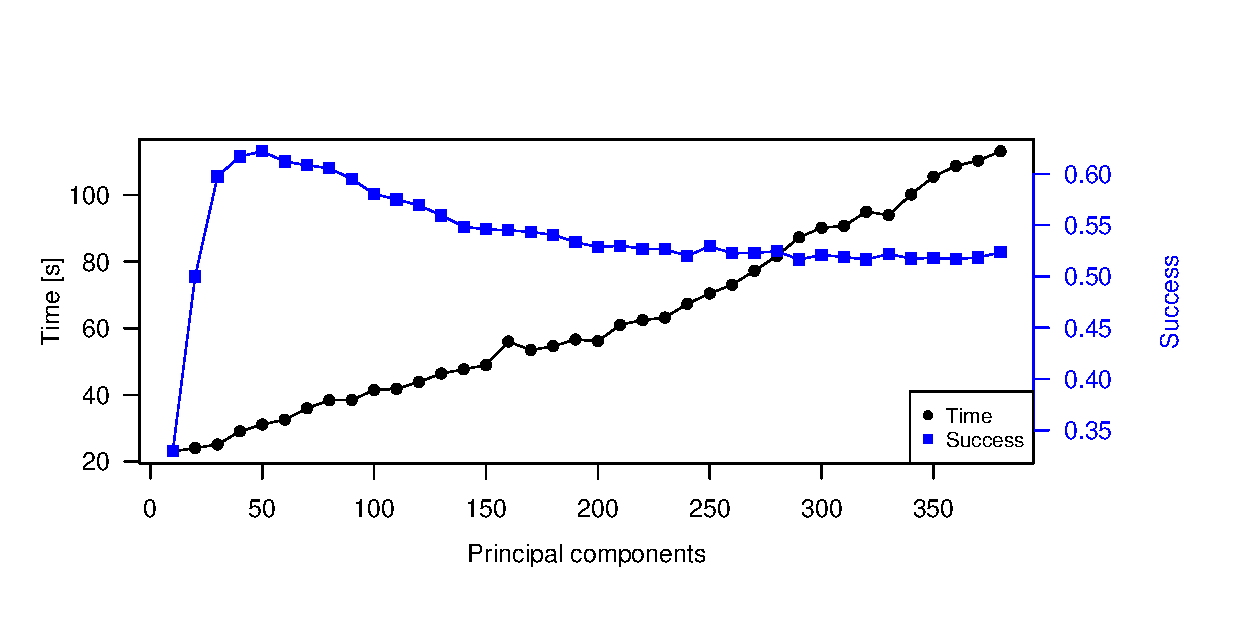
\includegraphics[width =0.8 \textwidth]{graphics/pca_timing_nikolaj}
\caption[Timing of PCA]{Timing of running the PCA with different principle components. 
The data was run on Group 3 member 1's data}
\label{fig:pca_timing_nikolaj}
\end{figure}

To get a closer look at how the PCA performs the data from G3M2 was tested against the rest of the class. 
The K was chosen to be 10. 
The data is shown in figure \ref{fig:pca_success}.
The performance is getting worse as more features are considered.

\begin{figure}[H]
\centering
\missingfigure{pca variance (acc. + non) when using zscore before}
\end{figure}





\newpage
\section{K-NN}
\section{Introduction}
The classification of handwritten characters is used in a wide range of products to day.
Hence, this report goes in depth with how the numbers from zero to nine can be classified using machine learning algorithms.

The dataset consists of a set of handwritten characters from zero to nine.
These were constructed by the students enrolled in the course Statistical Machine learning (RM-SML-E1) of the year 2015 at the University of Southern Denmark (SDU).
The set used in this report is the 100DPI dataset.
Each number is hence stored as a $20px \times 20px$ matrix containing the handwritten character.

The methods used for classification are K-Nearest Neighbours and Decision Trees and Random Forests.
Furthermore a set of different ways to pre-process the data is explored.
Finally the two methods are compared with each at the best parameters and preprocessing settings.





\subsection{Theory}
The K-Nearest Neighbour (K-NN) method is in this report used to classify a unknown digit to a set of known digits ranging from zero to nine.
%The data is split into two groups: One is for training and one is for testing. 
A set of the $k$ nearest neighbour is found using the euclidean distance to the pixel values in a training set of which the elements are already classified.
The result from the classification is found by counting the number of occurrences from the set of the $k$ nearest neighbours and choosing the most prominent.

%To see how this method performs a multitude of tests are performed to see how multiple parameters affect the success rate and the speed.

An example of such is seen in figure \ref{fig:knn_illustration}.

\begin{figure}[H]
\centering
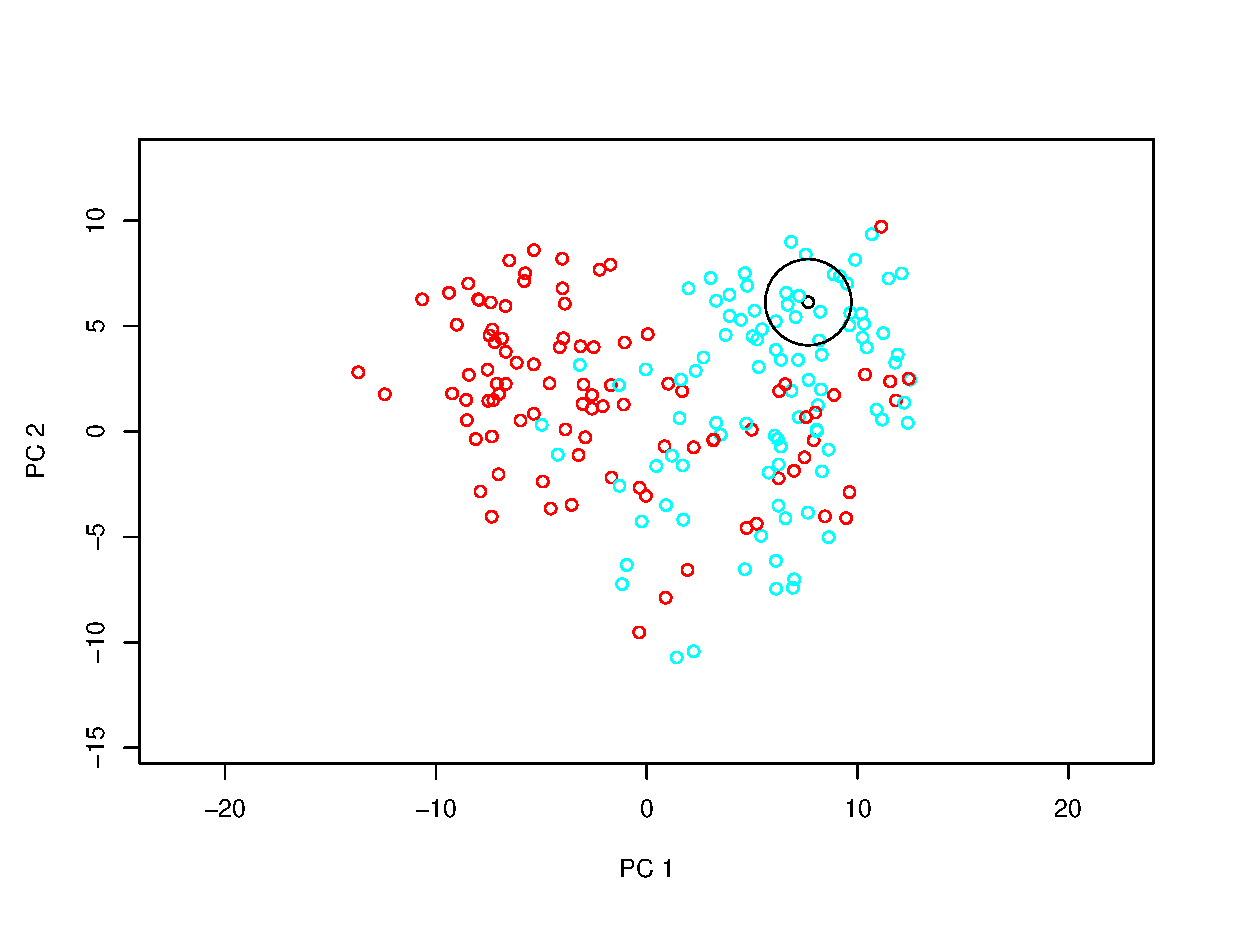
\includegraphics[width = 0.8 \textwidth]{graphics/knn_vis}
\caption[Illustration of the K-NN approach.]{Illustration of the K-NN approach with $k = 10$ on the normalized data for two classes plotting the two most prominent principle components.}
\label{fig:knn_illustration}
\end{figure}

In figure \ref{fig:knn_illustration} the black data point is an element of the blue test set.
The circle around it encircles the ten nearest neighbours.
Since there are more blue neighbours within the circle than red, then the classification in this case correctly classifies the element to the blue one.

\todo[inline]{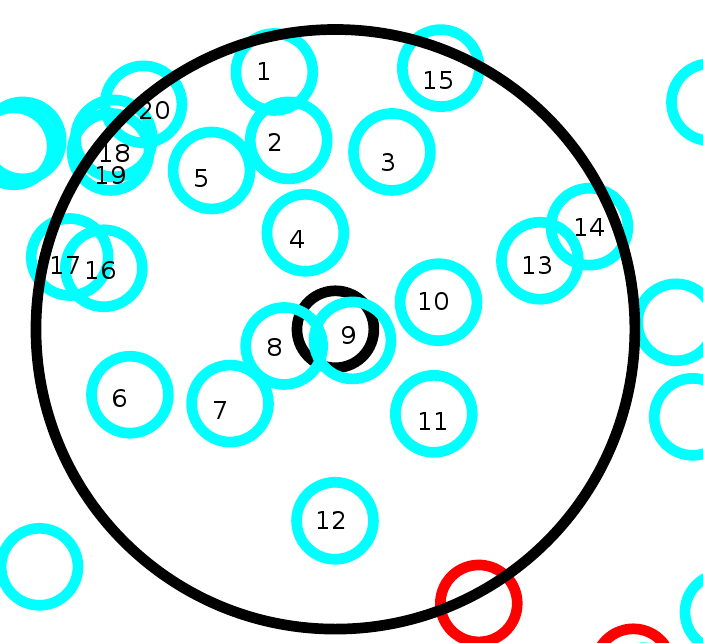
\includegraphics[width=0.2\textwidth]{graphics/knn_circle} Kan vi lave en cirkel om de 10 nærmeste?}
\subsection{Parameter Tuning}
The parameter tuning is important to the test because if not tuned correctly, the preprocessing methods will make the classification worse.
It was therefore decided to test the individual methods one by one and to possibly find the best setting.

\subsubsection{Raw Performance}
The parameter tuning for the pure K-NN is performed using the dataset of G3M2.
This was done because using a single persons dataset alone creates a clearer change in performance when comparing the scores.
Furthermore the reduced dataset makes it possible to test a larger set of parameters in less time.
The dataset was split in a $90\%/10\%$ split for training and test respectively.

To find the optimal value for $K$, figure \ref{fig:k_success}.

\begin{figure}[H]
\centering
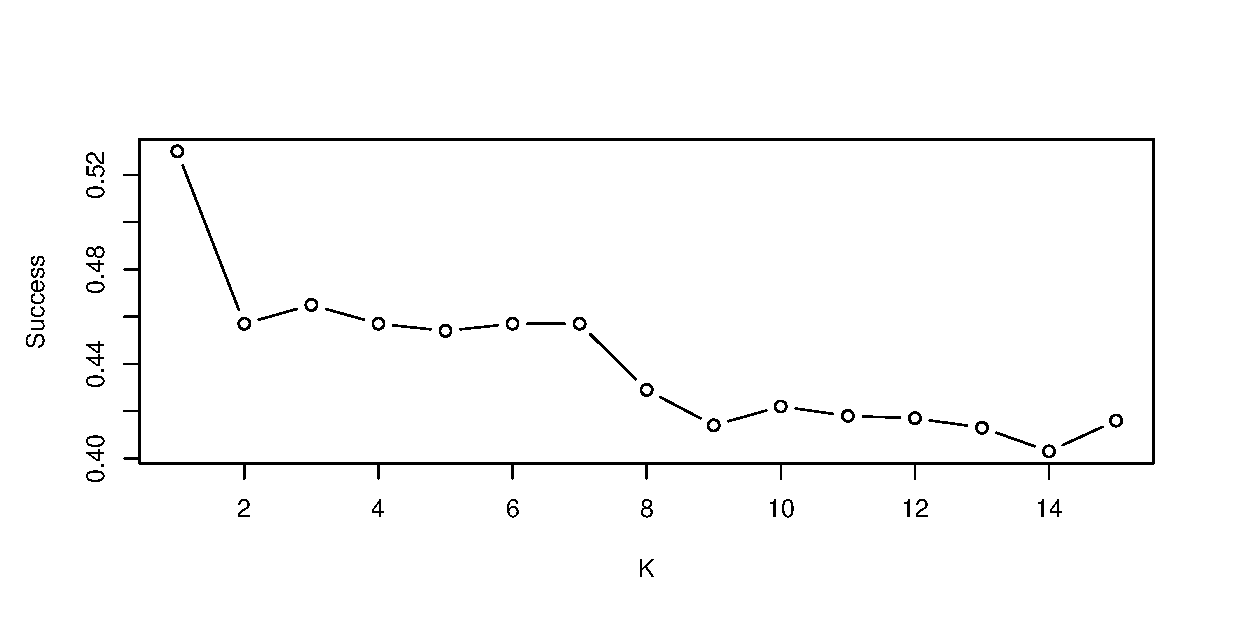
\includegraphics[width = 0.95 \textwidth]{graphics/knn_raw_success}
\caption{Success for K-NN with no preprocessing used.}
\label{fig:k_success}
\end{figure}

The best value for $K$ can from figure \ref{fig:k_success} be found to be $K = 1$.
For further test the value of $K = 1$ will hence be applied.
The same dataset is also for a range of the first initiating tests.


\subsubsection{Smoothing}
\label{sec:knn_smooth}
To find the best filter, the Gaussian filer is used.
As described earlier in section \ref{sec:smoothing}, then the Gaussian filter only has two parameters.
These are the kernel size and sigma.
When varying the sigma and kernel size, the contour in figure \ref{fig:cont_smooth_gaus_knn} is gained.

\begin{figure}[H]
\centering
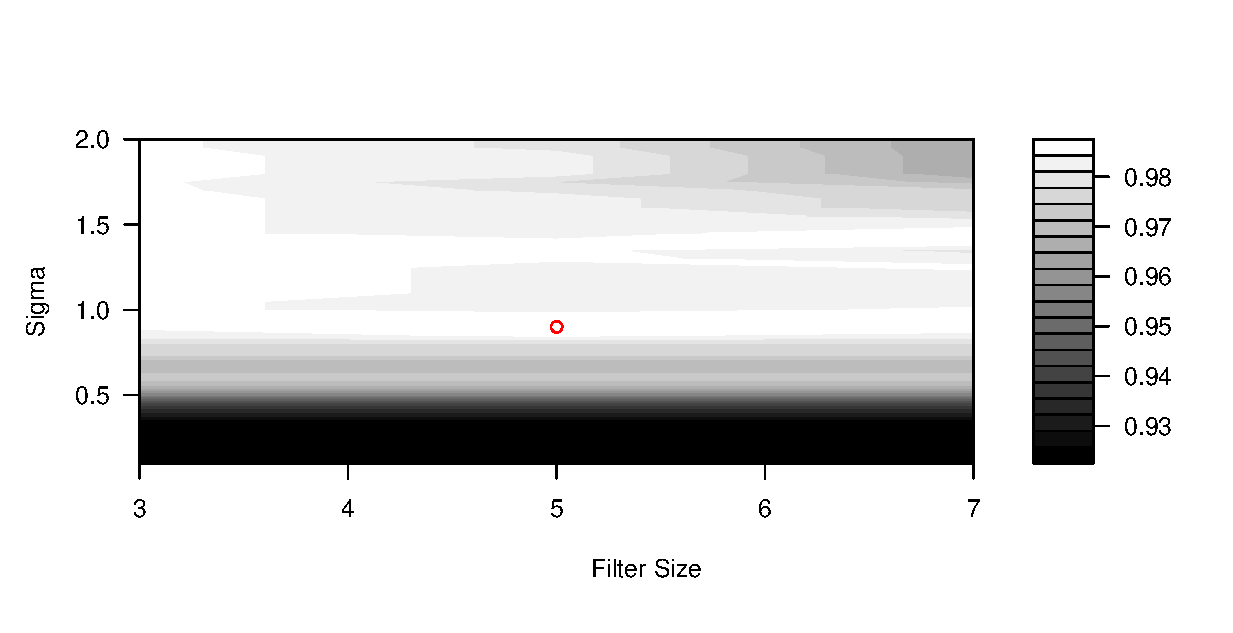
\includegraphics[width = 0.95 \textwidth]{graphics/knn_smooth_cont}
\caption[Success for K-NN with smoothing and PCA.]{Success for K-NN when the image is smoothed using a Gaussian filter with different kernel sizes and sigma values.}
\label{fig:cont_smooth_gaus_knn}
\end{figure}

The best point in figure \ref{fig:cont_smooth_gaus_knn} is highlighted with the red circle.
This is at $\sigma = 0.9$ and a kernel size of five.
This sigma and kernel size will hence be the one used onwards in this section when smoothing is done on the data before using K-NN.


\subsubsection{Principle Component Analysis}

The PCA was computed on the same dataset as in section \ref{sec:knn_smooth}.
The test where done on both the dataset with and without smoothing.
The result of plotting the number of PC versus the success and time taken to perform K-NN is seen on figure \ref{fig:plot_pca_knn}.

\begin{figure}[H]
\centering
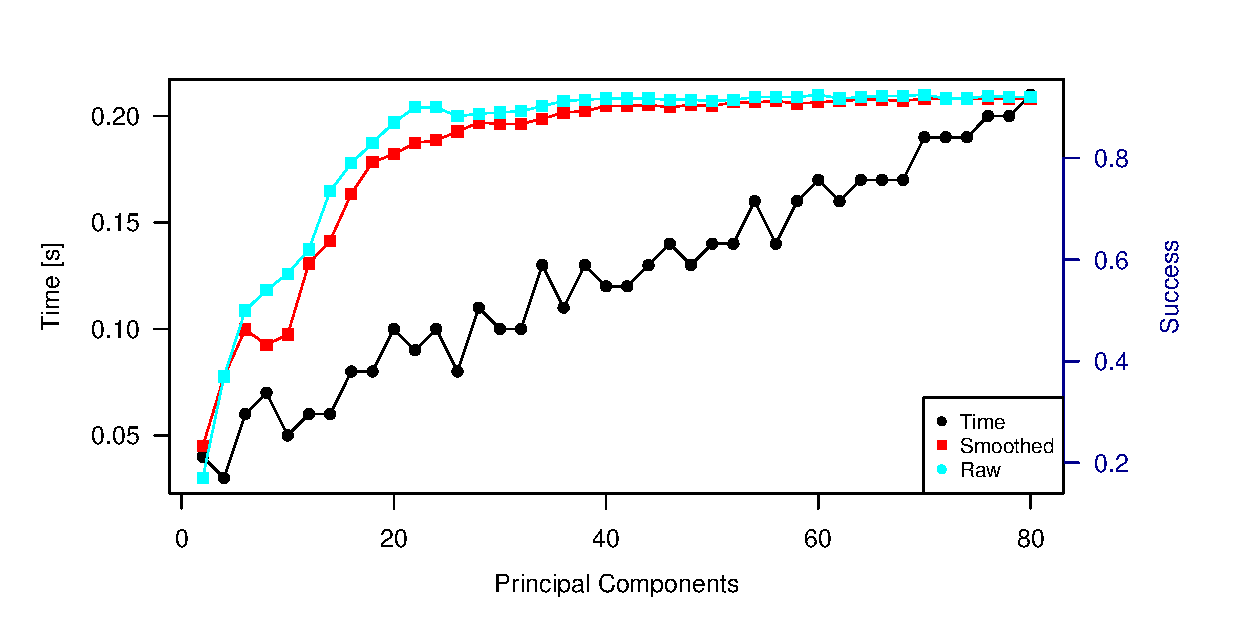
\includegraphics[width = 0.95 \textwidth]{graphics/knn_pc}
\caption{Success for K-NN for varying numbers of PC and sigma.}
\label{fig:plot_pca_knn}
\end{figure}


%Calculating with less data will result in a faster computation time.
%However, choosing too few PC results too few features left to compare.
%To see how the performance and the timing scales both are shown in figure \ref{fig:pca_timing_lukas} and \ref{fig:pca_timing_nikolaj}. K was chosen to be 10.
%In figure \ref{fig:pca_timing_lukas} the performance seems to be the same regardless of how many PC is chosen. As long as there are more than 60 the performance will be the same.
%On the test done on Group member 1 the performance is worse which means the digits are less uniform. 
%Here the success rate has a peak with a low set of attributes so there must be some confusion that gets sorted out. 
%Both test were run with 100 DPI. The percentage of successful predictions is also measured with the same data.
%The timing was measured on the same computer so the difference should not be very large. 

%To get a closer look at how the PCA performs the data from G3M2 was tested against the rest of the class. 
%The K was chosen to be 10. 
%The data is shown in figure \ref{fig:pca_success}.
%The performance is getting worse as more features are considered.


From figure \ref{fig:plot_pca_knn}, it was decided to use 40 PC.
This point was chosen because it efficiently reduces the dimensions of the dataset, but also has a descend success rate for the K-NN both with and without smoothing.
Furthermore the elbow-point is passed and no significant gain is gathered from taking more PC, compared to the timing advantage.



\subsubsection{Z-Score}
Z-score can be applied in a different number of ways.
This includes before PCA is made, after, both or not at all.
Furthermore this can be expanded to be used with and without smoothing and PCA.
This gives rise to 12 different ways in which the data can be processed.
Using the parameters for K-NN, PCA and smoothing, then the success rate of the different preprocessing methods can be computed.

The computations are done using three different datasets.
Once the dataset from the previous tests are used, the result of such is seen in figure \ref{fig:knn_zscore_1}.

A reduced dataset mixed with all peoples dataset can be used.
This is created taking 100 and 50 data points from each person into the test and train set respectively for each character.
Only one dataset was created (no cross-referencing).
The result of this is seen in figure \ref{fig:knn_zscore_2}.

The are also completed on the hard problem.
Here only 100 data points from one persons data was selected as the test set and 50 from each of the remaining people for the training set, for each character.
This gave the result in figure \ref{fig:knn_zscore_3}.


\begin{figure}[H]
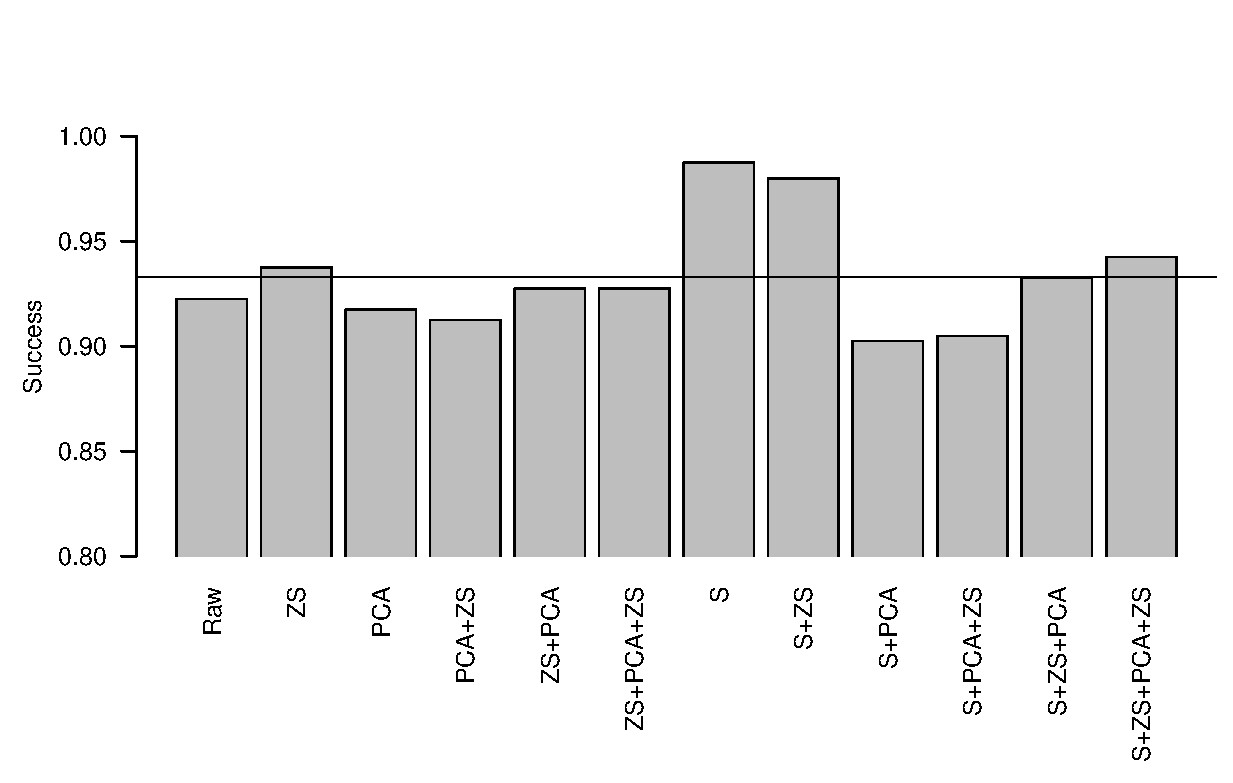
\includegraphics[width = 0.95 \textwidth]{graphics/knn_zscore_1}
\caption[Success for K-NN with different preprocessing schemes. Simplified problem.]{Success for the K-NN algorithm for one persons dataset. Different preprocessing schemes used.
Where $S$ is smoothing, $ZS$ is z-score.
The preprocessing schemes are named in the same order as applied.}
\label{fig:knn_zscore_1}
\end{figure}

\begin{figure}[H]
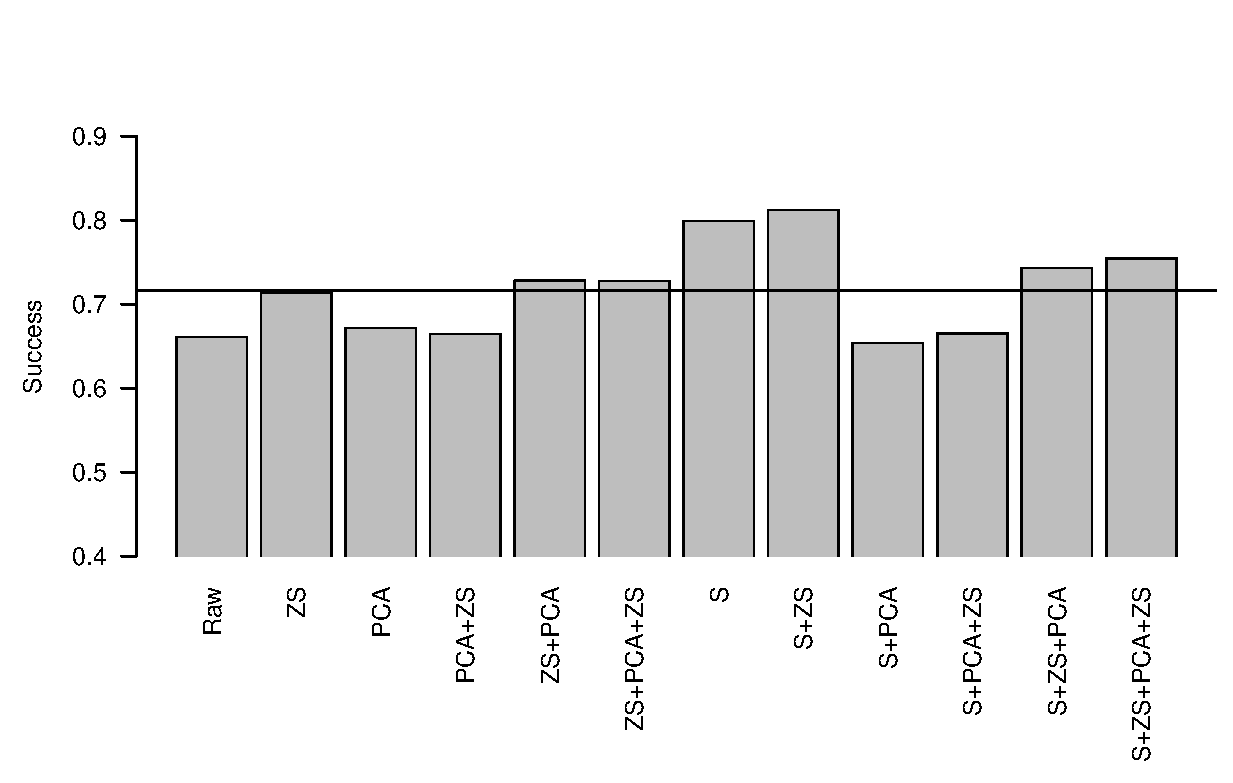
\includegraphics[width = 0.95 \textwidth]{graphics/knn_zscore_2}
\caption[Success for K-NN with different preprocessing schemes. Easy problem.]{Success for the K-NN algorithm for all peoples datasets mixed (easy problem no cross-referencing). Different preprocessing schemes used.
Where $S$ is smoothing, $ZS$ is z-score.
The preprocessing schemes are named in the same order as applied.}
\label{fig:knn_zscore_2}
\end{figure}

\begin{figure}[H]
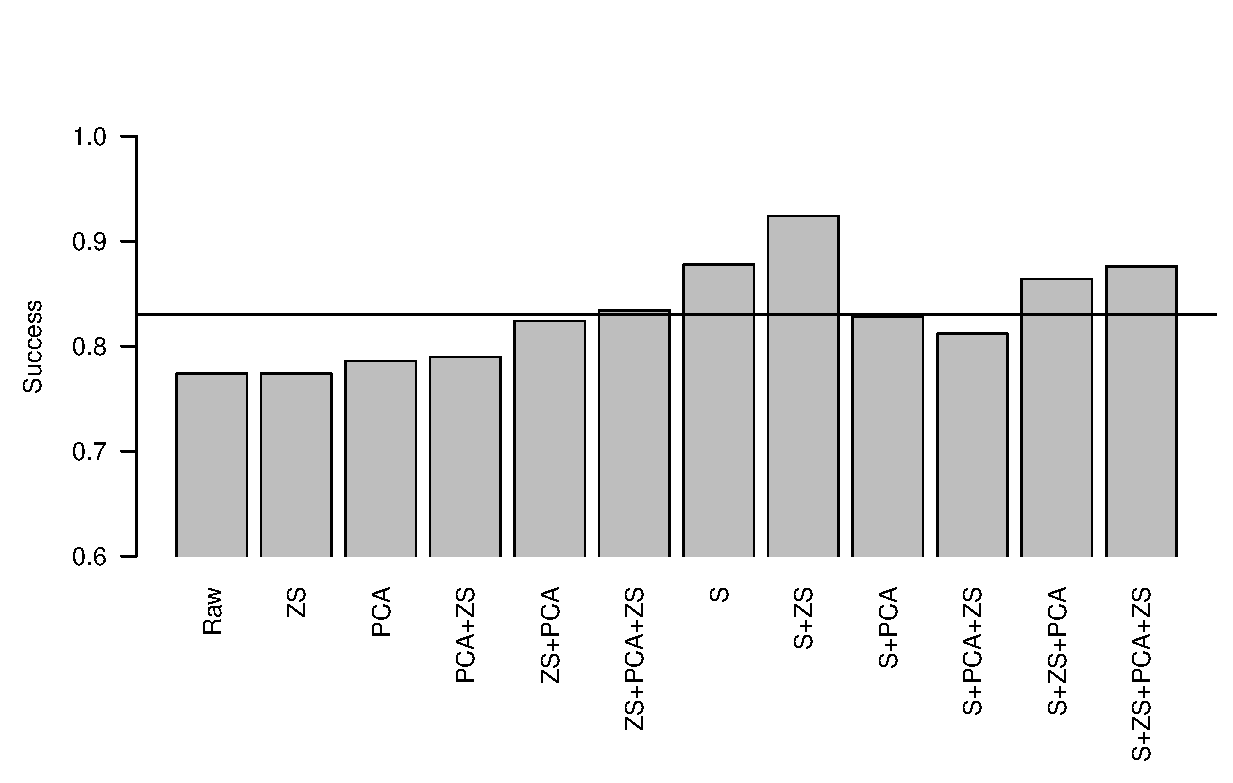
\includegraphics[width = 0.95 \textwidth]{graphics/knn_zscore_3}
\caption[Success for K-NN with different preprocessing schemes. Hard problem.]{Success for the K-NN algorithm for one person vs the rest (hard problem for G3M2 only). Different preprocessing schemes used.
Where $S$ is smoothing, $ZS$ is z-score.
The preprocessing schemes are named in the same order as applied.}
\label{fig:knn_zscore_3}
\end{figure}


As expected, all the test with PCA perform worse than those without as the dataset is heavily reduced.

To decide further which of the methods to use, then the timing of two best methods will be considered next.
%Because of the reduced computational time when using PCA, it is chosen to use one of the methods including PCA.
%Furthermore, then the success rate drop by using PCA is not of such a significant level that PCA is not beneficial.
%
%Considering the three figures \ref{fig:knn_zscore_1}, \ref{fig:knn_zscore_2} and \ref{fig:knn_zscore_3}, then it was chosen to use preprocessing scheme with smoothing and z-score both before and after PCA.
%This was chosen as it gives the highest success of all the schemes including PCA.


\subsection{Timing}

To test the performance of the two best methods, measured in success, these were timed to find the time they take to compute.
Figure \ref{fig:knn_timing_comp} shows the result of such.

The dataset used is one in which the dataset of G3M2 is used as the test set and the remaining 19 peoples dataset is contained in the training set.


\begin{figure}[H]
\centering
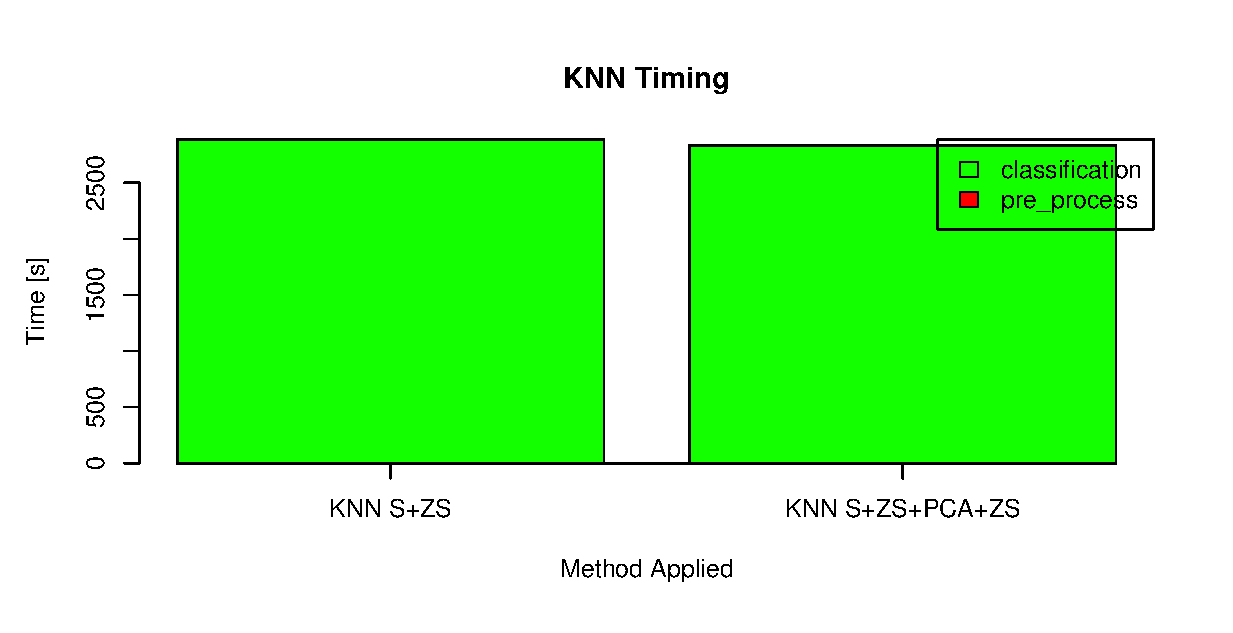
\includegraphics[width =  \textwidth]{graphics/compare_timing_knn_smoothVSpca}
\caption[Time distribution for K-NN.]{Time distribution of the preprocessing and classification time of the KNN algorithm in the two run modes.}
\label{fig:knn_timing_comp}
\end{figure}

The timing was computed for both the preprocessing of the testing set and the thereafter following classification using the data generated.
As seen on figure \ref{fig:knn_timing_comp} then the data preprocessed with PCA is more than 100 times faster than the data which was only smoothed and normalized.
It was therefore decided to use the reduced dataset to reduce the time taken to compute the classifications.


\subsubsection{Performance}

To test the overall performance with the final parameters, both confusion tables and success using K-NN with the beforehand decided preprocessing was computed.
Both the hard problem and the easy problem was computed.

The easy problem is the one in which the data from the different people is divided into a 90\%/10\% split, training and test respectively.
The test and training sets of each person are then combined.
This was done for ten cross-validation runs.
The result of such procedure can be seen in figure \ref{fig:knn_succ_final_easy}, where the success for the ten runs is shown in a boxplot, and figure \ref{fig:knn_conf_final_easy} shows the overall confusion matrix for all ten runs combined.


\begin{figure}[H]
\centering
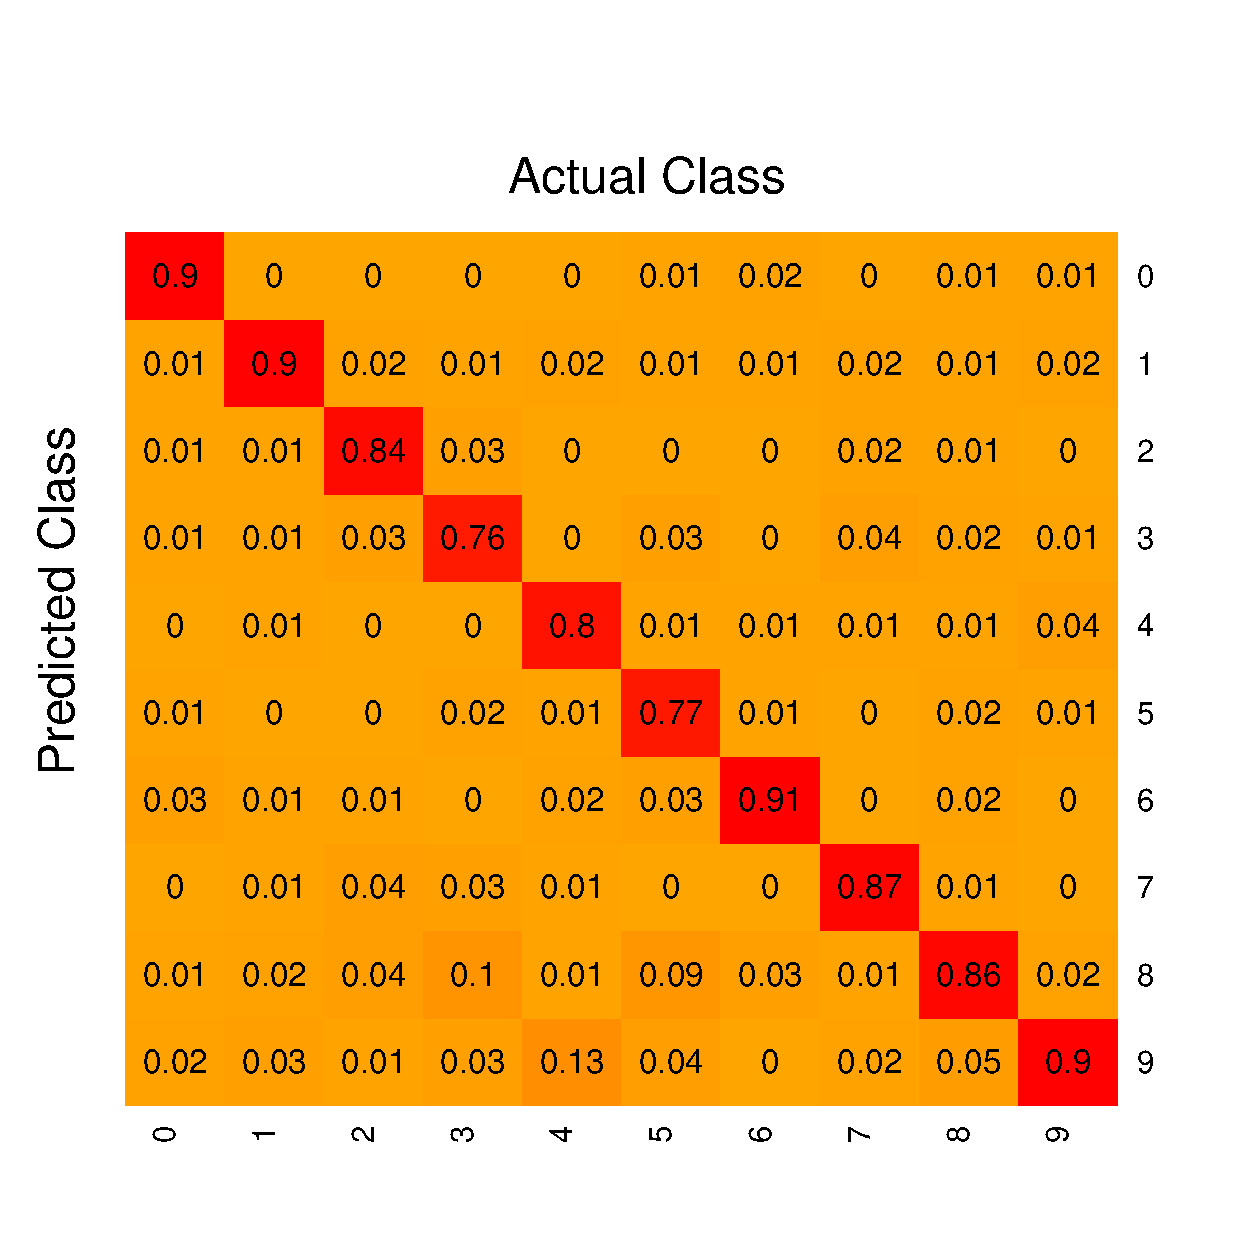
\includegraphics[width = 0.65 \textwidth]{graphics/knn_confusion_bestparam_easy}
\caption[Confusion table for the easy problem.]{Confusion table of the best parameter setting, for the easy problem with ten cross referencing runs.}
\label{fig:knn_conf_final_easy}
\end{figure}


\begin{figure}[H]
\centering
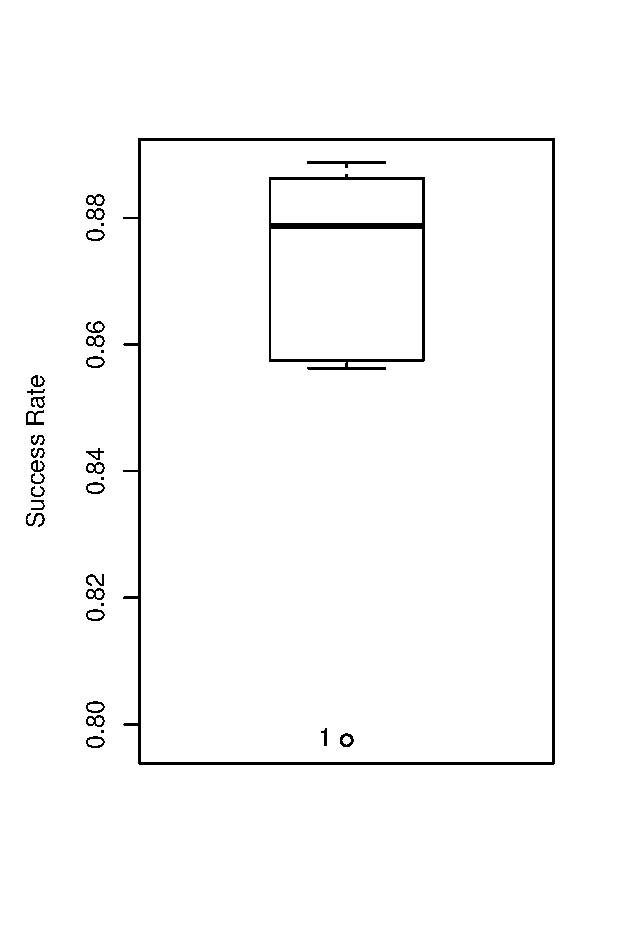
\includegraphics[width = 0.9 \textwidth]{graphics/knn_final_full_easy}
\caption[Success of K-NN on the easy problem.]{Success for the easy problem using ten cross referencing runs.}
\label{fig:knn_succ_final_easy}
\end{figure}


The hard problem is the one in which one persons test data was used as the test data alone and the remaining peoples put together in the training set.
This was done for all people with all the data present, such that each person once was used as the test set.
The success of such a process is seen in figure \ref{fig:knn_succ_final_hard} and figure \ref{fig:knn_conf_final_hard} shows the overall confusion table, when the confusion tables of each run was put together.


\begin{figure}[H]
\centering
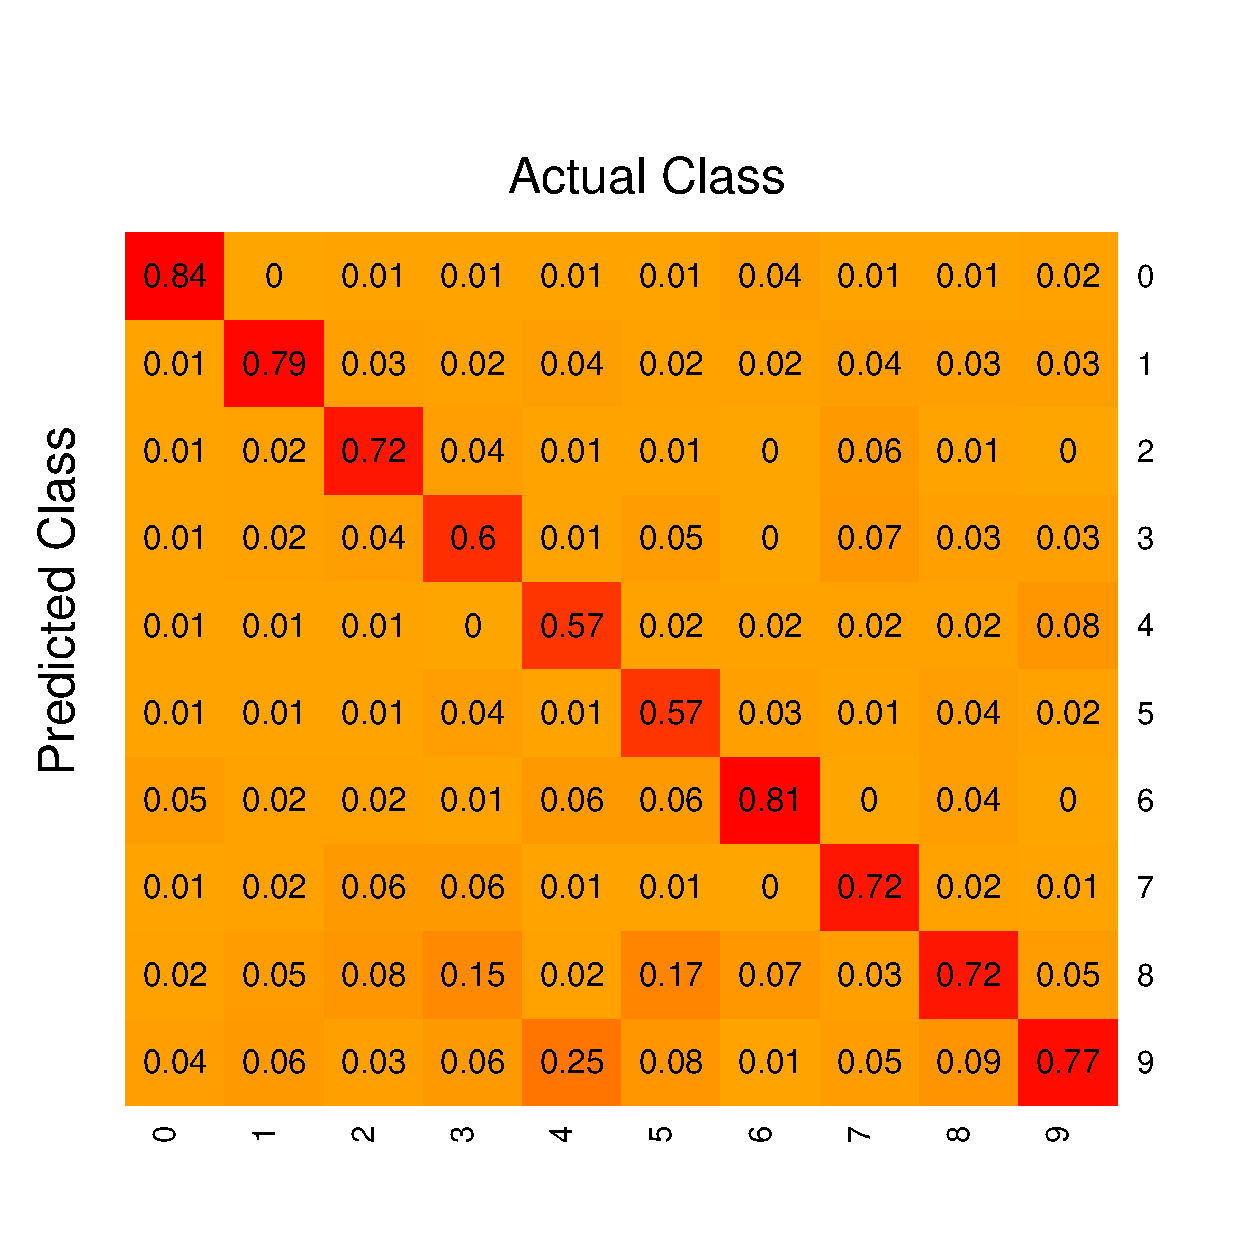
\includegraphics[width = 0.65 \textwidth]{graphics/knn_confusion_bestparam_hard}
\caption[Confusion table for the hard problem.]{Confusion table with all the best parameters for the full dataset difficult problem with the confusion tables for the different runs combined.}
\label{fig:knn_conf_final_hard}
\end{figure}


\begin{figure}[H]
\centering
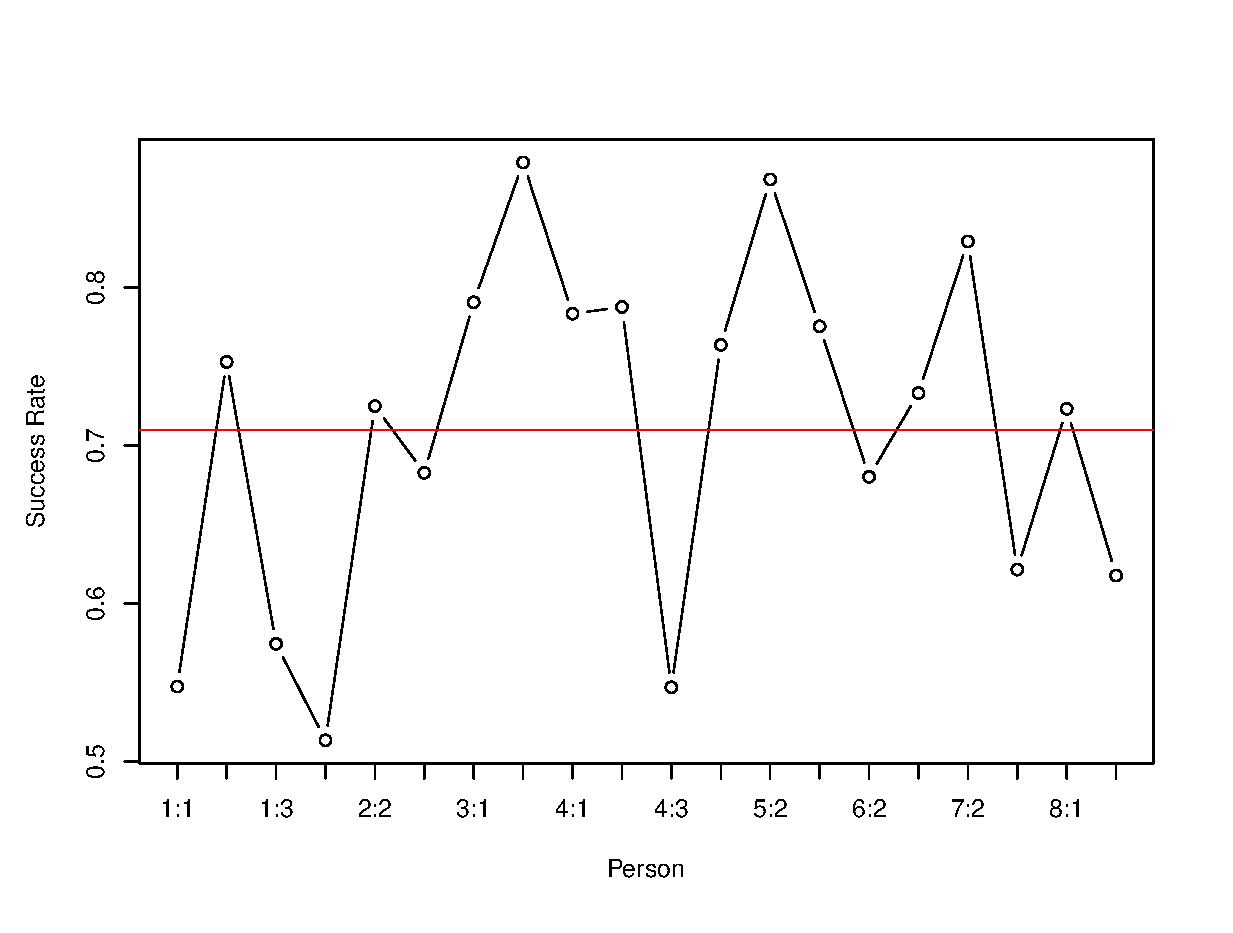
\includegraphics[width = 0.95 \textwidth]{graphics/knn_final_full_hard}
\caption[Success for K-NN for the hard problem.]{Success for the hard problem for each person.
The y-axis values represents the "Group:Member" number used as the test set.}
\label{fig:knn_succ_final_hard}
\end{figure}

With a mean of $70.99\%$ and variance of  $117.81\%^2$, then the hard problem clearly performs worse than the easy problem with $85.07\%$ mean and $3.59\%^2$ variance.
The general tendency is that the greatest error comes from the '3' and '5' often being detected as '8', and the '4' being classified as a '9'.
These two errors account for 5.7\% and 3.3\% of the error in hard and easy problem respectively, and is hence more than 1/6 in the two classification problems.
This is, however, expected as the characters of confusion have great similarity compared to any other class in the dataset.


\subsection{Conclusion}
It can be found that the optimal preprossing of the data for decision trees is
smoothing, then
z-score, then
PCA with 130 chosen components,
Boosting with 7 trials, and removal of leaves with less than 7 digits.

G2M1
has been found to have the worst handwriting when comparing the data of all people.




\newpage
\section{Decision Trees}
\section{Introduction}
The classification of handwritten characters is used in a wide range of products to day.
Hence, this report goes in depth with how the numbers from zero to nine can be classified using machine learning algorithms.

The dataset consists of a set of handwritten characters from zero to nine.
These were constructed by the students enrolled in the course Statistical Machine learning (RM-SML-E1) of the year 2015 at the University of Southern Denmark (SDU).
The set used in this report is the 100DPI dataset.
Each number is hence stored as a $20px \times 20px$ matrix containing the handwritten character.

The methods used for classification are K-Nearest Neighbours and Decision Trees and Random Forests.
Furthermore a set of different ways to pre-process the data is explored.
Finally the two methods are compared with each at the best parameters and preprocessing settings.





\subsection{Entropy}
To compute the optimum decision point for the individual principle components, the entropy method is used.
The entropy of the PC's with our ten ciphers is given by equation \ref{eq:entropy}.

\begin{equation}
Entropy(S) = \sum_{i = '0'}^{'9'} -p_i \cdot \log_2(p_i) 
\qquad \because p_i = P(x = i)
\label{eq:entropy}
\end{equation}

To find the best decision point, it is wished that the entropy of the two resulting systems, when dividing one PC into two, is as low as possible.
This can be represented as sum of entropy for our two resulting datasets, weighted by the relative size of such.
This is given in equation \ref{eq:entropy_datasetdevision}.

\begin{eqnarray}
Entropy = \sum_{i = 1}^{2} \frac{s_i \cdot Entropy(S_i)}{\sum_{k = 1}^{2} s_k} 
\qquad \because S_i \subset S\ and\ s_k = size(S_k)
\label{eq:entropy_datasetdevision}
\end{eqnarray}

When using equation \ref{eq:entropy_datasetdevision} on the first five principle components on the data of 15 people from the class, then figure \ref{fig:entropy_pc5} was gained.

\begin{figure}[H]
\centering
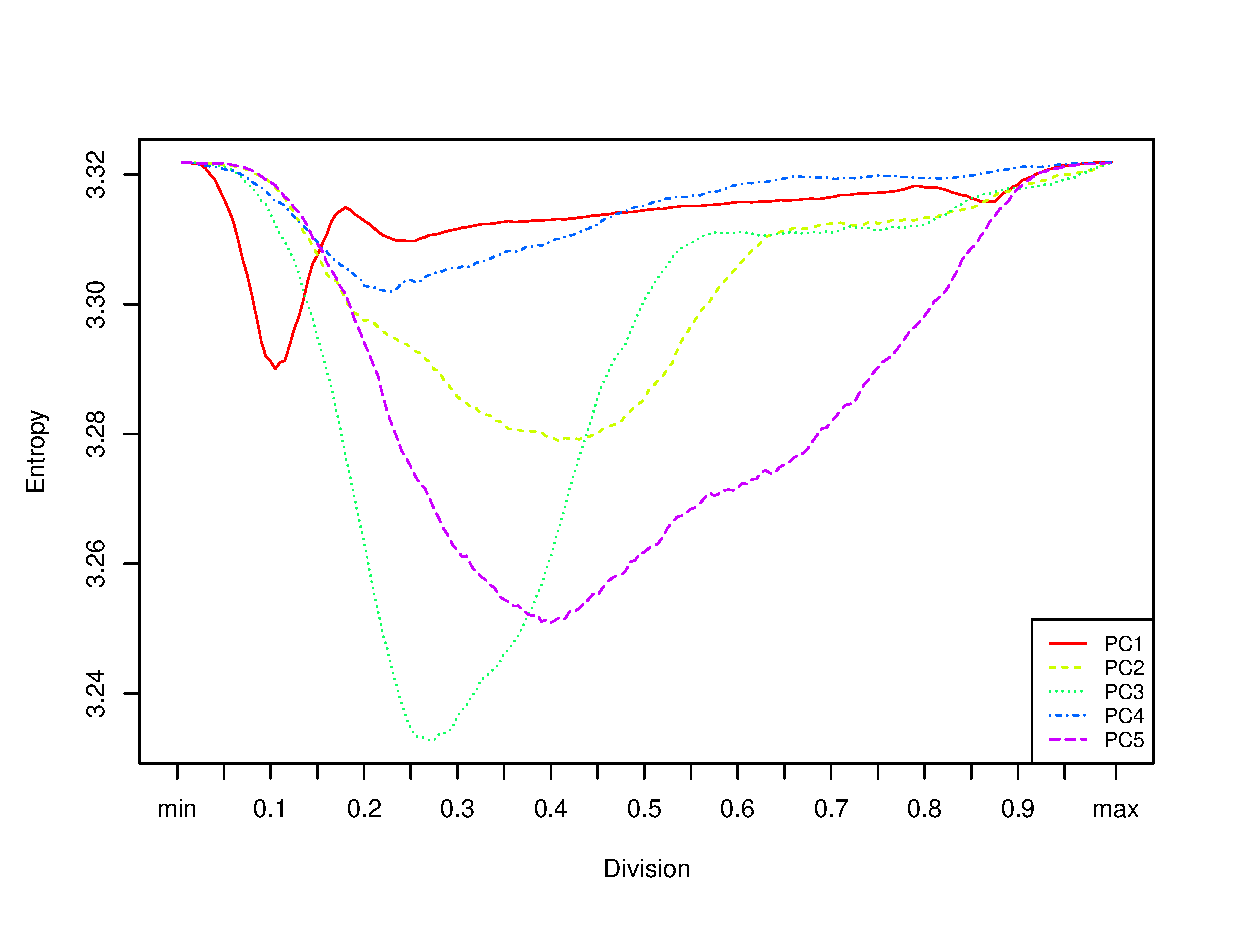
\includegraphics[width = 0.95 \textwidth]{graphics/entropy_pc}
\caption{Figure showing the variation of the entropy of the dataset when the decision point varies. Computed using equation \ref{eq:entropy_datasetdevision}. The data of the first five principle component.}
\label{fig:entropy_pc5}
\end{figure}


The point of lowest entropy for a principle component was then used as the splitting point to convert the data into binary.
This was done by setting everything below the splitting point to true and the rest false.
This was then done for all principle components on both the test and train set. 
The splitting point for the components in the test set were taken as the splitting point from the same component in the train set.

The optimal decision decision point is shown along with the PC values for PC1 in figure \ref{fig:decision_point}. 
Here it is clear that if the data is above the split then it can not be a 0.
If the data is below, further investigation is needed.
By removing all unlikely classes the true class must remain.

\begin{figure}[H]
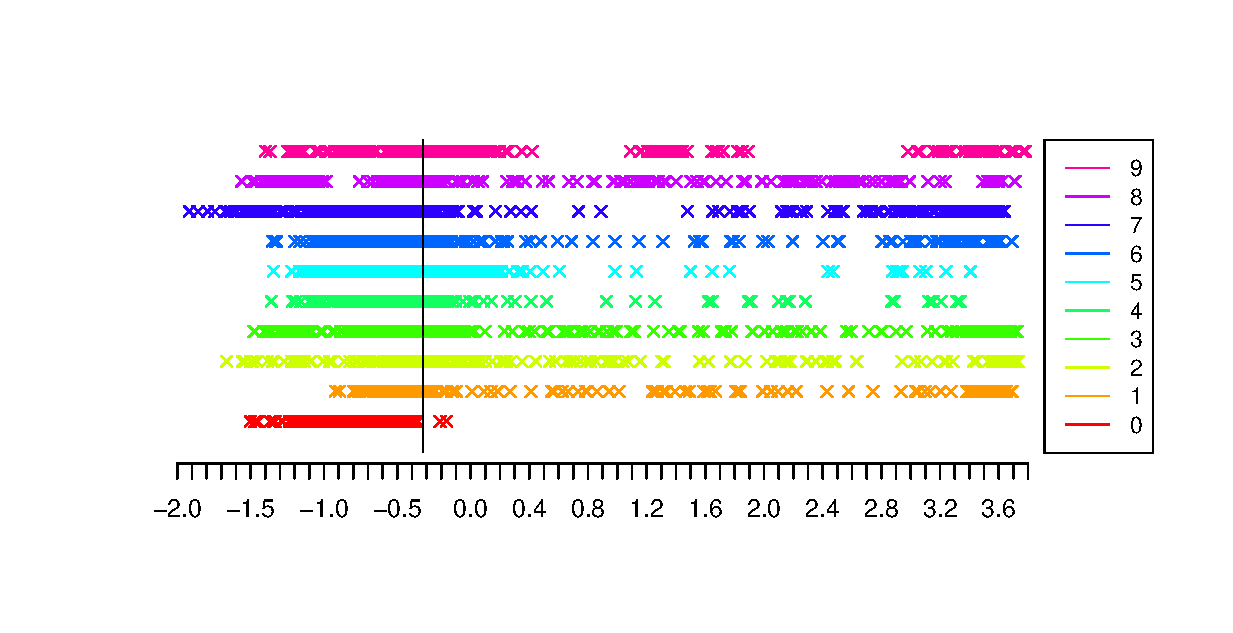
\includegraphics[width = \textwidth]{graphics/decision_seperation}
\caption{Decision point in relation to PC values}
\label{fig:decision_point}
\end{figure}
\subsection{Theory}
The K-Nearest Neighbour (K-NN) method is in this report used to classify a unknown digit to a set of known digits ranging from zero to nine.
%The data is split into two groups: One is for training and one is for testing. 
A set of the $k$ nearest neighbour is found using the euclidean distance to the pixel values in a training set of which the elements are already classified.
The result from the classification is found by counting the number of occurrences from the set of the $k$ nearest neighbours and choosing the most prominent.

%To see how this method performs a multitude of tests are performed to see how multiple parameters affect the success rate and the speed.

An example of such is seen in figure \ref{fig:knn_illustration}.

\begin{figure}[H]
\centering
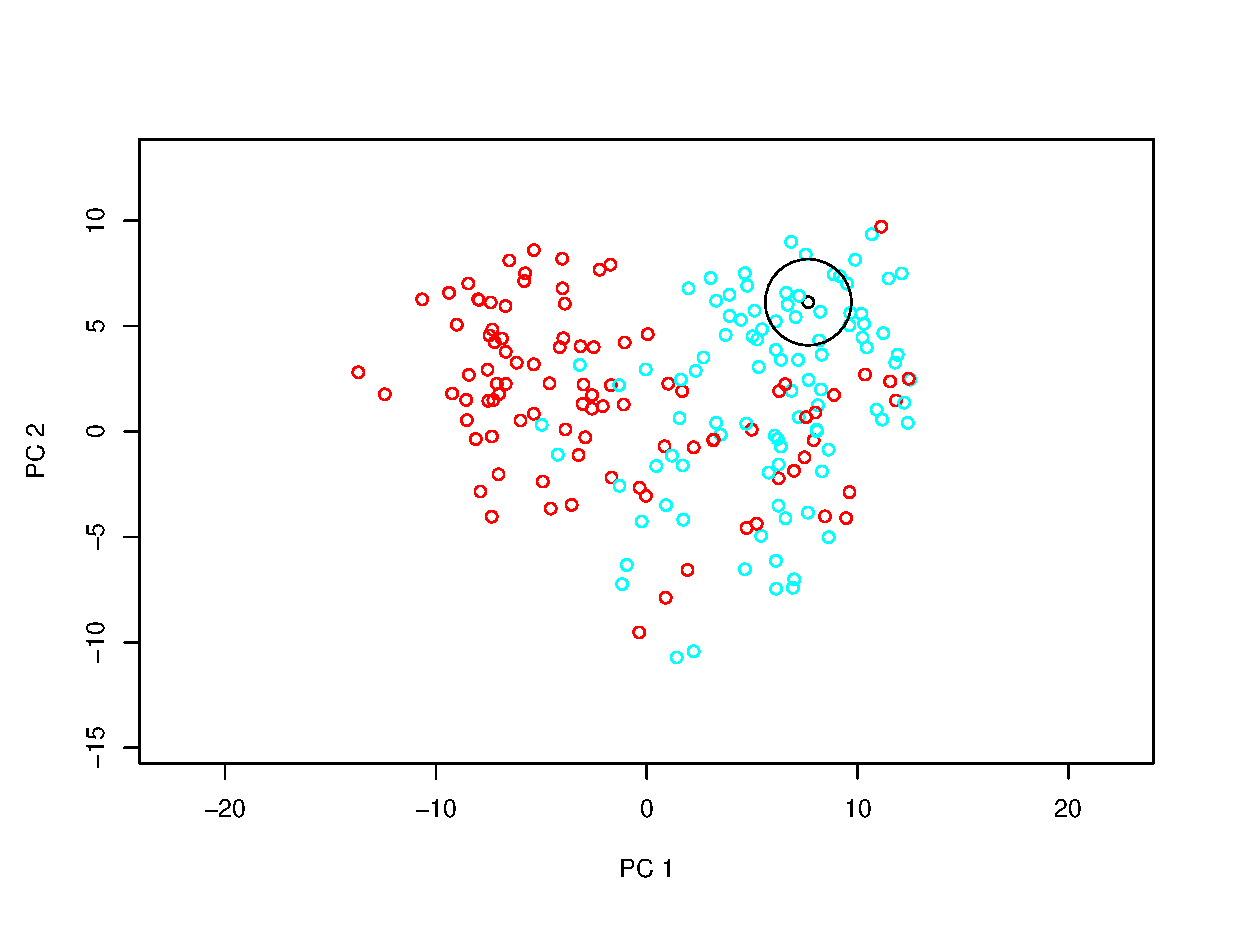
\includegraphics[width = 0.8 \textwidth]{graphics/knn_vis}
\caption[Illustration of the K-NN approach.]{Illustration of the K-NN approach with $k = 10$ on the normalized data for two classes plotting the two most prominent principle components.}
\label{fig:knn_illustration}
\end{figure}

In figure \ref{fig:knn_illustration} the black data point is an element of the blue test set.
The circle around it encircles the ten nearest neighbours.
Since there are more blue neighbours within the circle than red, then the classification in this case correctly classifies the element to the blue one.

\todo[inline]{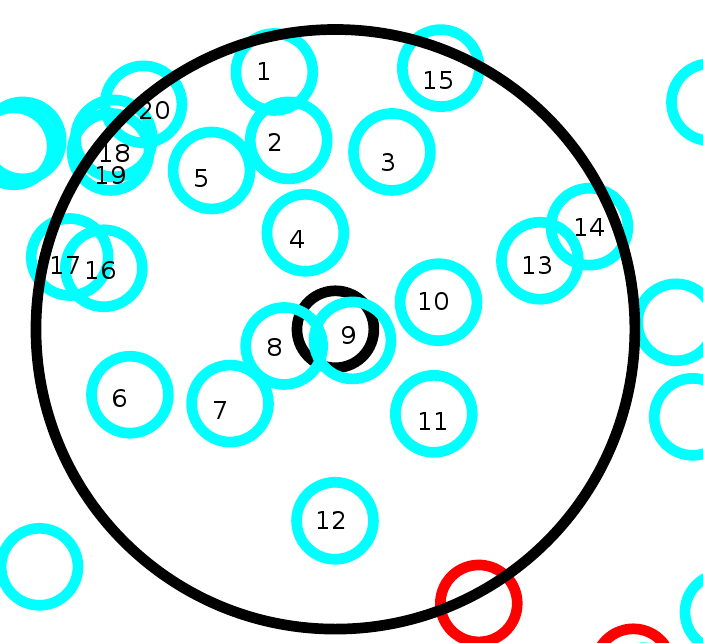
\includegraphics[width=0.2\textwidth]{graphics/knn_circle} Kan vi lave en cirkel om de 10 nærmeste?}
\subsection{Parameter Tuning}
The parameter tuning is important to the test because if not tuned correctly, the preprocessing methods will make the classification worse.
It was therefore decided to test the individual methods one by one and to possibly find the best setting.

\subsubsection{Raw Performance}
The parameter tuning for the pure K-NN is performed using the dataset of G3M2.
This was done because using a single persons dataset alone creates a clearer change in performance when comparing the scores.
Furthermore the reduced dataset makes it possible to test a larger set of parameters in less time.
The dataset was split in a $90\%/10\%$ split for training and test respectively.

To find the optimal value for $K$, figure \ref{fig:k_success}.

\begin{figure}[H]
\centering
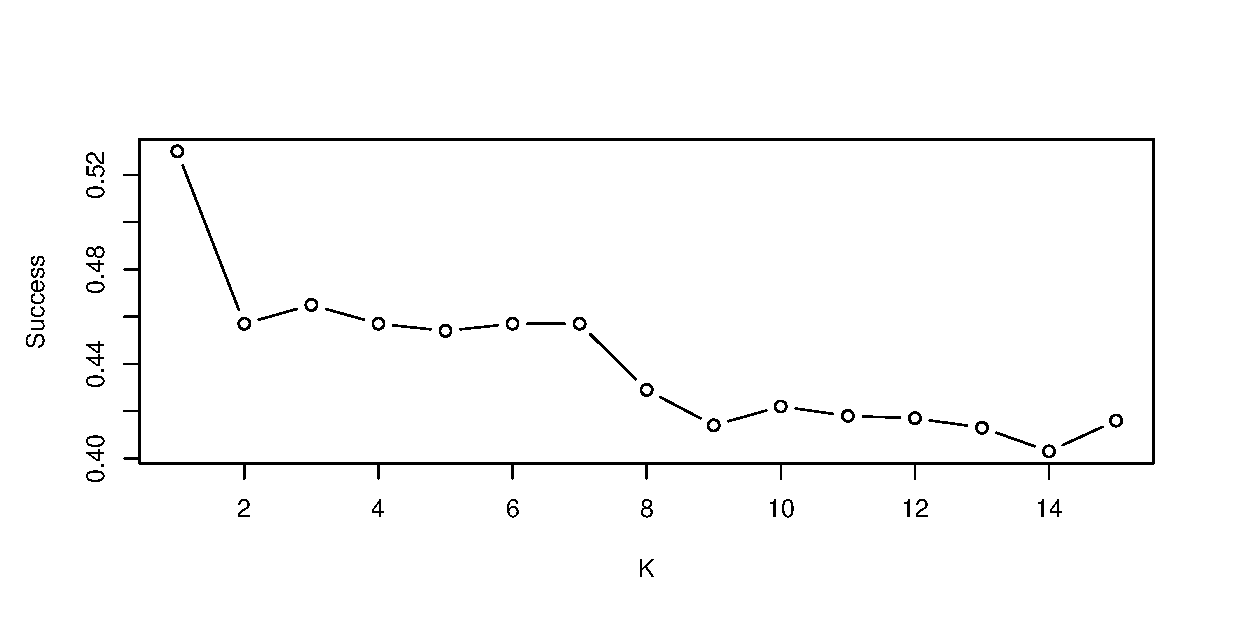
\includegraphics[width = 0.95 \textwidth]{graphics/knn_raw_success}
\caption{Success for K-NN with no preprocessing used.}
\label{fig:k_success}
\end{figure}

The best value for $K$ can from figure \ref{fig:k_success} be found to be $K = 1$.
For further test the value of $K = 1$ will hence be applied.
The same dataset is also for a range of the first initiating tests.


\subsubsection{Smoothing}
\label{sec:knn_smooth}
To find the best filter, the Gaussian filer is used.
As described earlier in section \ref{sec:smoothing}, then the Gaussian filter only has two parameters.
These are the kernel size and sigma.
When varying the sigma and kernel size, the contour in figure \ref{fig:cont_smooth_gaus_knn} is gained.

\begin{figure}[H]
\centering
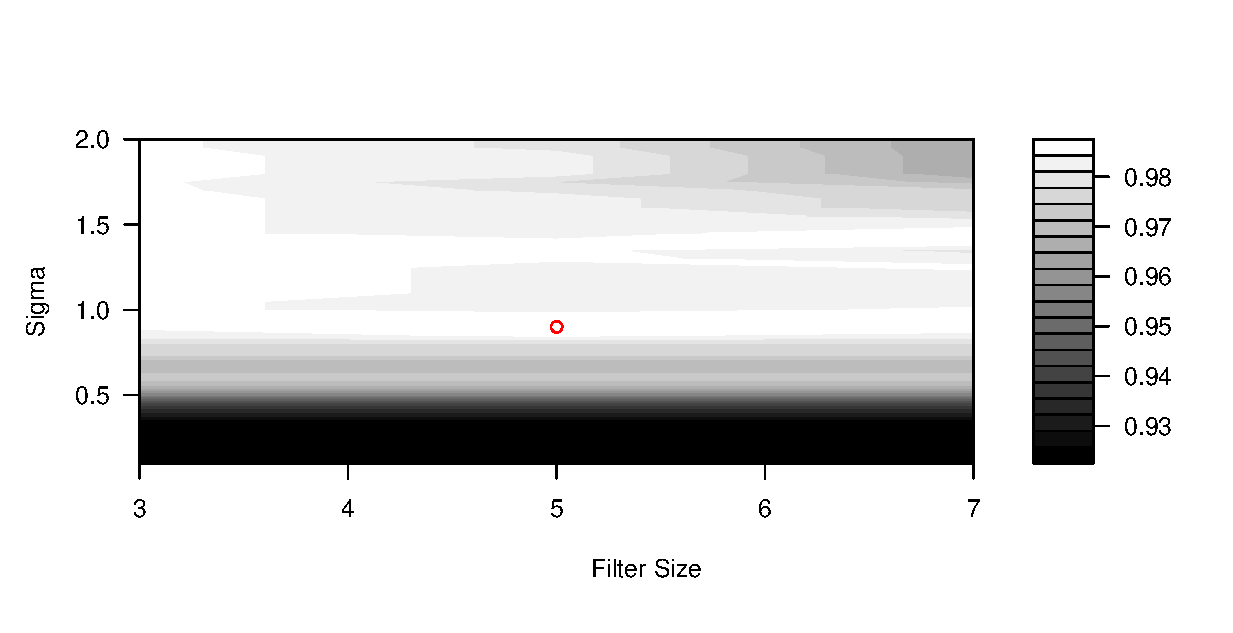
\includegraphics[width = 0.95 \textwidth]{graphics/knn_smooth_cont}
\caption[Success for K-NN with smoothing and PCA.]{Success for K-NN when the image is smoothed using a Gaussian filter with different kernel sizes and sigma values.}
\label{fig:cont_smooth_gaus_knn}
\end{figure}

The best point in figure \ref{fig:cont_smooth_gaus_knn} is highlighted with the red circle.
This is at $\sigma = 0.9$ and a kernel size of five.
This sigma and kernel size will hence be the one used onwards in this section when smoothing is done on the data before using K-NN.


\subsubsection{Principle Component Analysis}

The PCA was computed on the same dataset as in section \ref{sec:knn_smooth}.
The test where done on both the dataset with and without smoothing.
The result of plotting the number of PC versus the success and time taken to perform K-NN is seen on figure \ref{fig:plot_pca_knn}.

\begin{figure}[H]
\centering
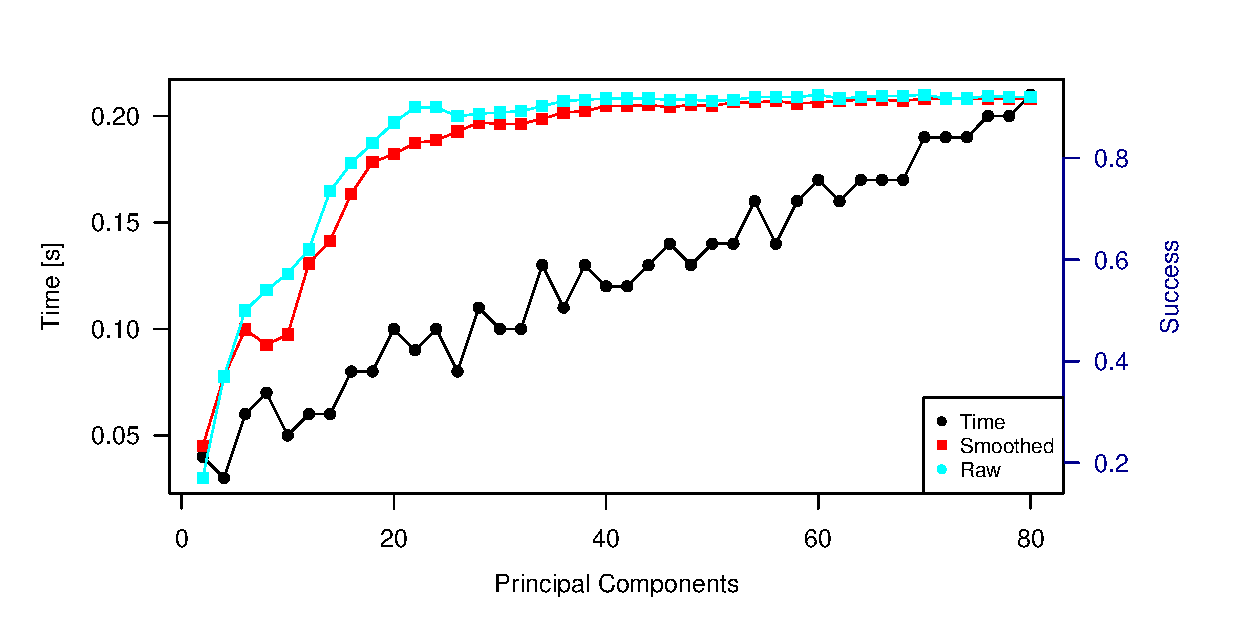
\includegraphics[width = 0.95 \textwidth]{graphics/knn_pc}
\caption{Success for K-NN for varying numbers of PC and sigma.}
\label{fig:plot_pca_knn}
\end{figure}


%Calculating with less data will result in a faster computation time.
%However, choosing too few PC results too few features left to compare.
%To see how the performance and the timing scales both are shown in figure \ref{fig:pca_timing_lukas} and \ref{fig:pca_timing_nikolaj}. K was chosen to be 10.
%In figure \ref{fig:pca_timing_lukas} the performance seems to be the same regardless of how many PC is chosen. As long as there are more than 60 the performance will be the same.
%On the test done on Group member 1 the performance is worse which means the digits are less uniform. 
%Here the success rate has a peak with a low set of attributes so there must be some confusion that gets sorted out. 
%Both test were run with 100 DPI. The percentage of successful predictions is also measured with the same data.
%The timing was measured on the same computer so the difference should not be very large. 

%To get a closer look at how the PCA performs the data from G3M2 was tested against the rest of the class. 
%The K was chosen to be 10. 
%The data is shown in figure \ref{fig:pca_success}.
%The performance is getting worse as more features are considered.


From figure \ref{fig:plot_pca_knn}, it was decided to use 40 PC.
This point was chosen because it efficiently reduces the dimensions of the dataset, but also has a descend success rate for the K-NN both with and without smoothing.
Furthermore the elbow-point is passed and no significant gain is gathered from taking more PC, compared to the timing advantage.



\subsubsection{Z-Score}
Z-score can be applied in a different number of ways.
This includes before PCA is made, after, both or not at all.
Furthermore this can be expanded to be used with and without smoothing and PCA.
This gives rise to 12 different ways in which the data can be processed.
Using the parameters for K-NN, PCA and smoothing, then the success rate of the different preprocessing methods can be computed.

The computations are done using three different datasets.
Once the dataset from the previous tests are used, the result of such is seen in figure \ref{fig:knn_zscore_1}.

A reduced dataset mixed with all peoples dataset can be used.
This is created taking 100 and 50 data points from each person into the test and train set respectively for each character.
Only one dataset was created (no cross-referencing).
The result of this is seen in figure \ref{fig:knn_zscore_2}.

The are also completed on the hard problem.
Here only 100 data points from one persons data was selected as the test set and 50 from each of the remaining people for the training set, for each character.
This gave the result in figure \ref{fig:knn_zscore_3}.


\begin{figure}[H]
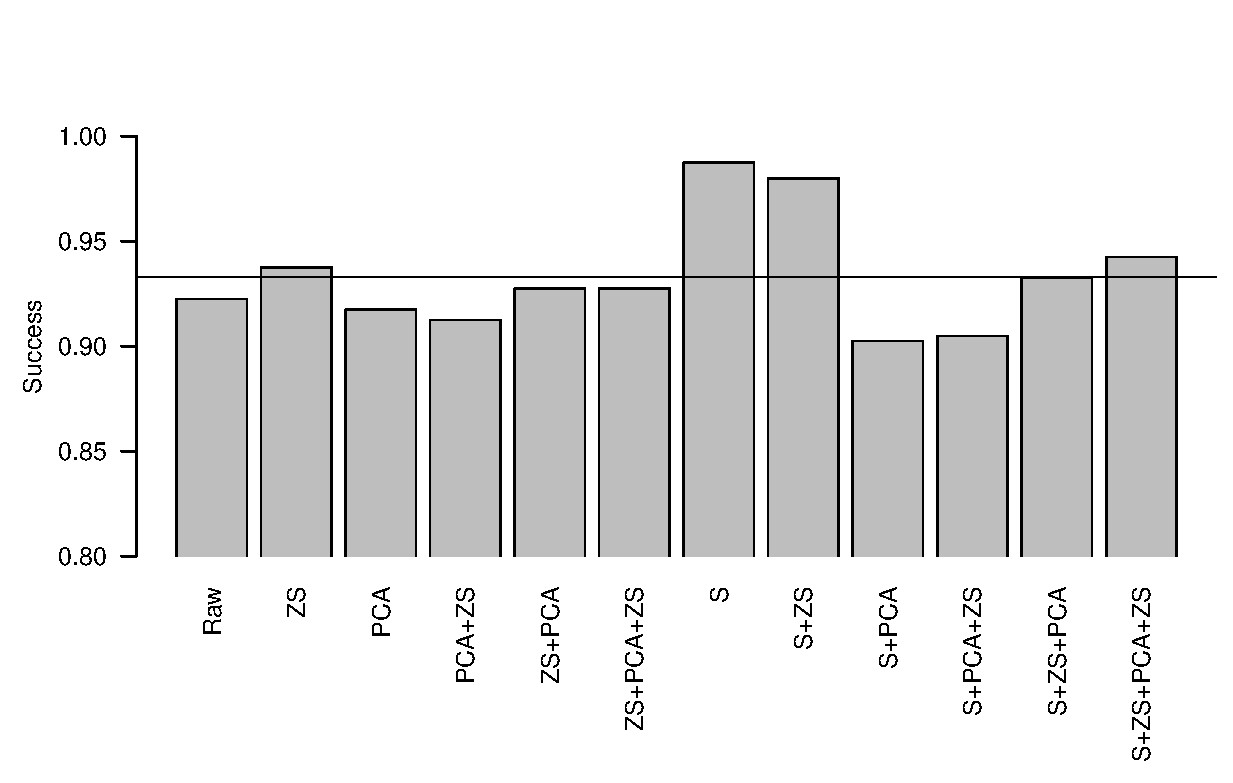
\includegraphics[width = 0.95 \textwidth]{graphics/knn_zscore_1}
\caption[Success for K-NN with different preprocessing schemes. Simplified problem.]{Success for the K-NN algorithm for one persons dataset. Different preprocessing schemes used.
Where $S$ is smoothing, $ZS$ is z-score.
The preprocessing schemes are named in the same order as applied.}
\label{fig:knn_zscore_1}
\end{figure}

\begin{figure}[H]
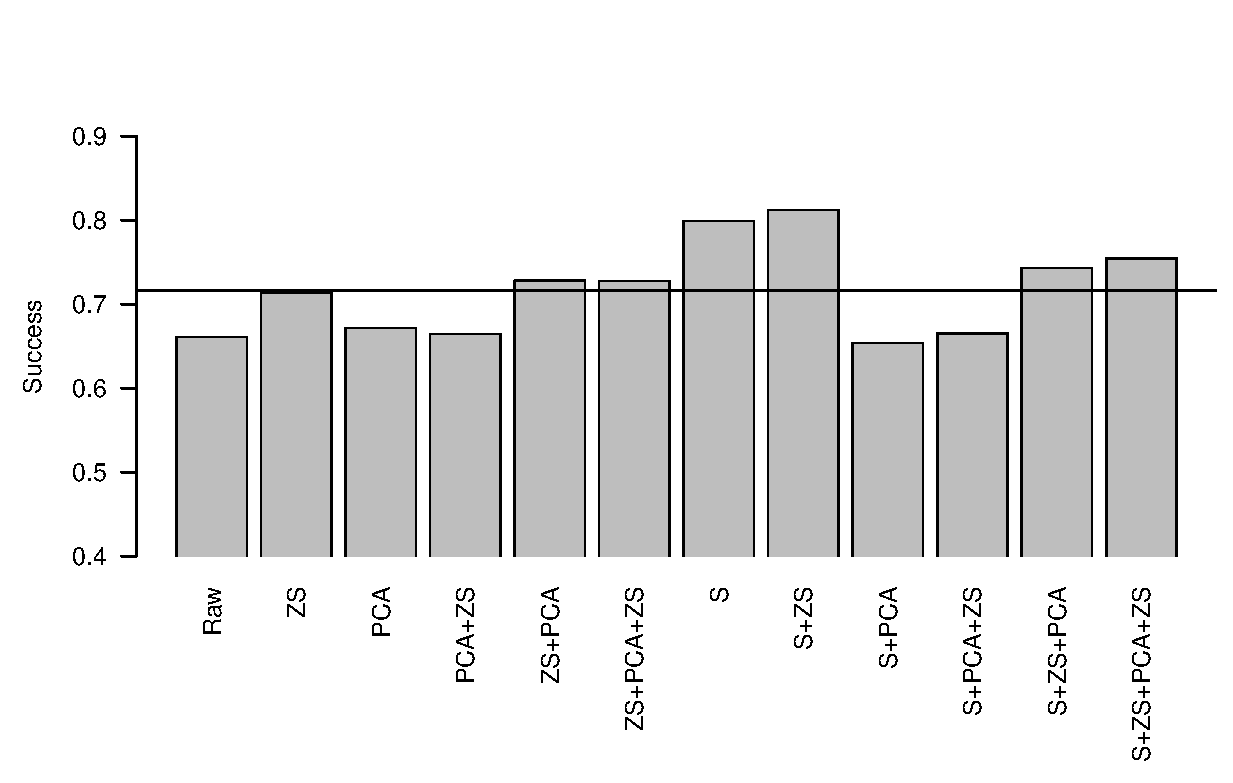
\includegraphics[width = 0.95 \textwidth]{graphics/knn_zscore_2}
\caption[Success for K-NN with different preprocessing schemes. Easy problem.]{Success for the K-NN algorithm for all peoples datasets mixed (easy problem no cross-referencing). Different preprocessing schemes used.
Where $S$ is smoothing, $ZS$ is z-score.
The preprocessing schemes are named in the same order as applied.}
\label{fig:knn_zscore_2}
\end{figure}

\begin{figure}[H]
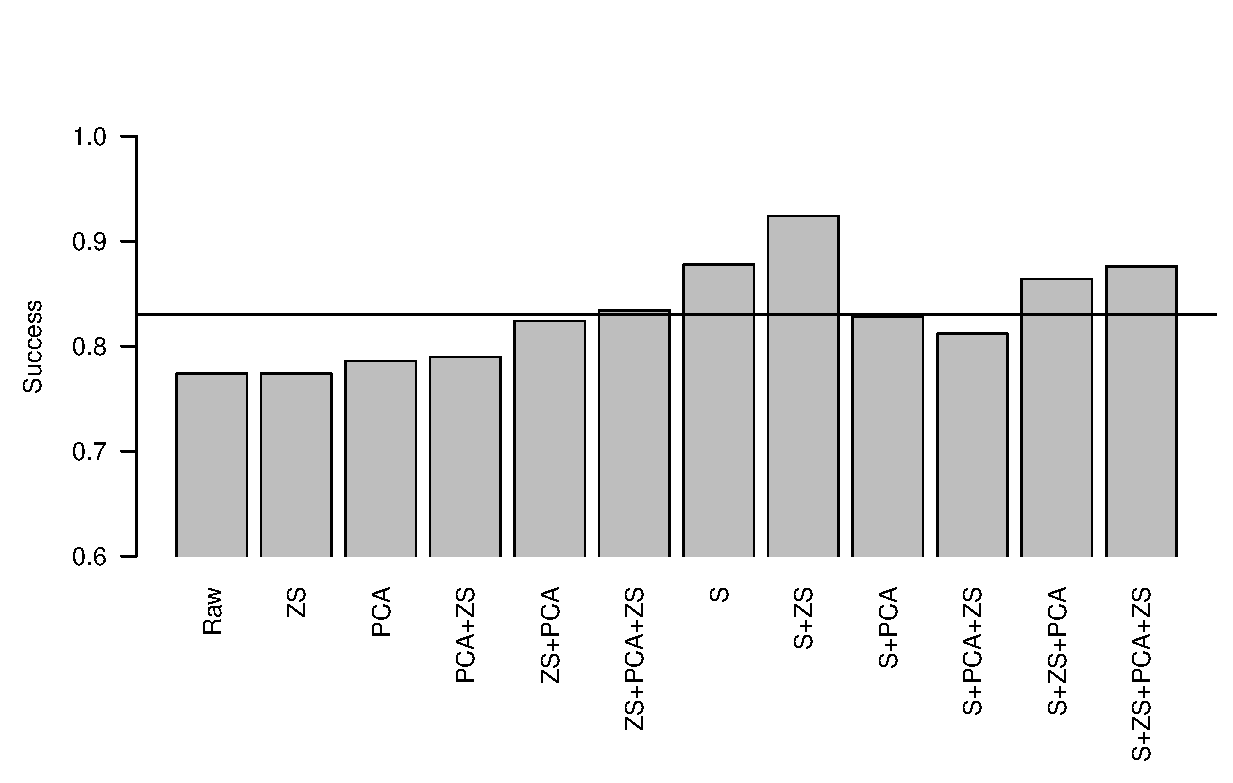
\includegraphics[width = 0.95 \textwidth]{graphics/knn_zscore_3}
\caption[Success for K-NN with different preprocessing schemes. Hard problem.]{Success for the K-NN algorithm for one person vs the rest (hard problem for G3M2 only). Different preprocessing schemes used.
Where $S$ is smoothing, $ZS$ is z-score.
The preprocessing schemes are named in the same order as applied.}
\label{fig:knn_zscore_3}
\end{figure}


As expected, all the test with PCA perform worse than those without as the dataset is heavily reduced.

To decide further which of the methods to use, then the timing of two best methods will be considered next.
%Because of the reduced computational time when using PCA, it is chosen to use one of the methods including PCA.
%Furthermore, then the success rate drop by using PCA is not of such a significant level that PCA is not beneficial.
%
%Considering the three figures \ref{fig:knn_zscore_1}, \ref{fig:knn_zscore_2} and \ref{fig:knn_zscore_3}, then it was chosen to use preprocessing scheme with smoothing and z-score both before and after PCA.
%This was chosen as it gives the highest success of all the schemes including PCA.


\subsection{Timing}

To test the performance of the two best methods, measured in success, these were timed to find the time they take to compute.
Figure \ref{fig:knn_timing_comp} shows the result of such.

The dataset used is one in which the dataset of G3M2 is used as the test set and the remaining 19 peoples dataset is contained in the training set.


\begin{figure}[H]
\centering
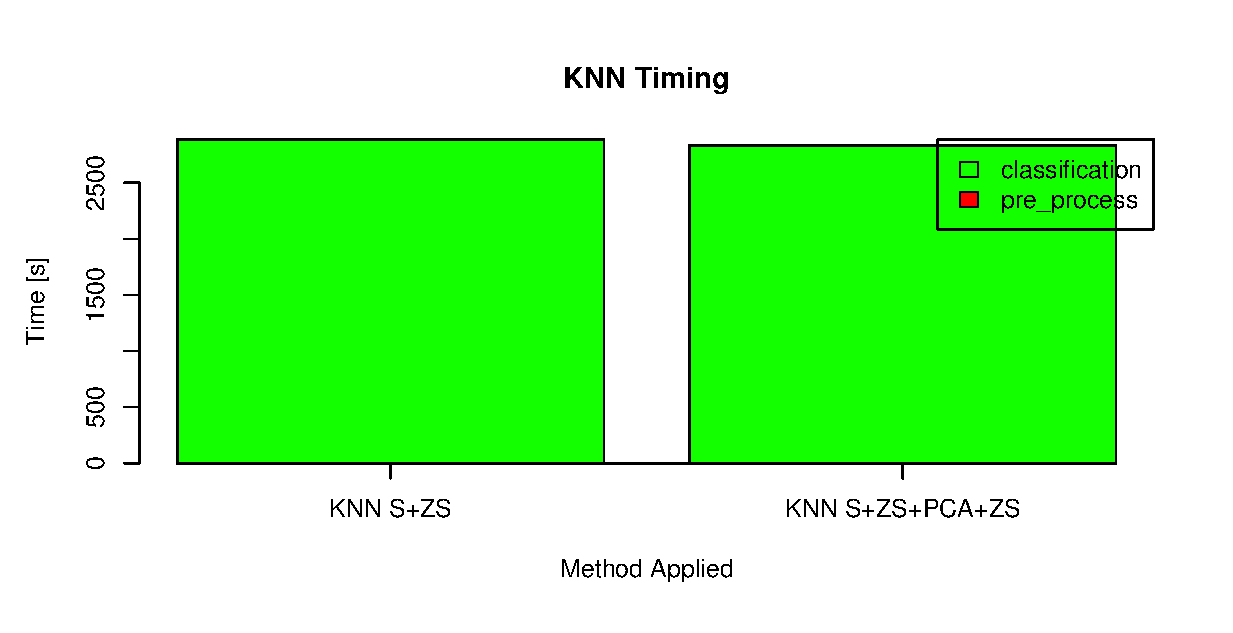
\includegraphics[width =  \textwidth]{graphics/compare_timing_knn_smoothVSpca}
\caption[Time distribution for K-NN.]{Time distribution of the preprocessing and classification time of the KNN algorithm in the two run modes.}
\label{fig:knn_timing_comp}
\end{figure}

The timing was computed for both the preprocessing of the testing set and the thereafter following classification using the data generated.
As seen on figure \ref{fig:knn_timing_comp} then the data preprocessed with PCA is more than 100 times faster than the data which was only smoothed and normalized.
It was therefore decided to use the reduced dataset to reduce the time taken to compute the classifications.


\subsubsection{Performance}

To test the overall performance with the final parameters, both confusion tables and success using K-NN with the beforehand decided preprocessing was computed.
Both the hard problem and the easy problem was computed.

The easy problem is the one in which the data from the different people is divided into a 90\%/10\% split, training and test respectively.
The test and training sets of each person are then combined.
This was done for ten cross-validation runs.
The result of such procedure can be seen in figure \ref{fig:knn_succ_final_easy}, where the success for the ten runs is shown in a boxplot, and figure \ref{fig:knn_conf_final_easy} shows the overall confusion matrix for all ten runs combined.


\begin{figure}[H]
\centering
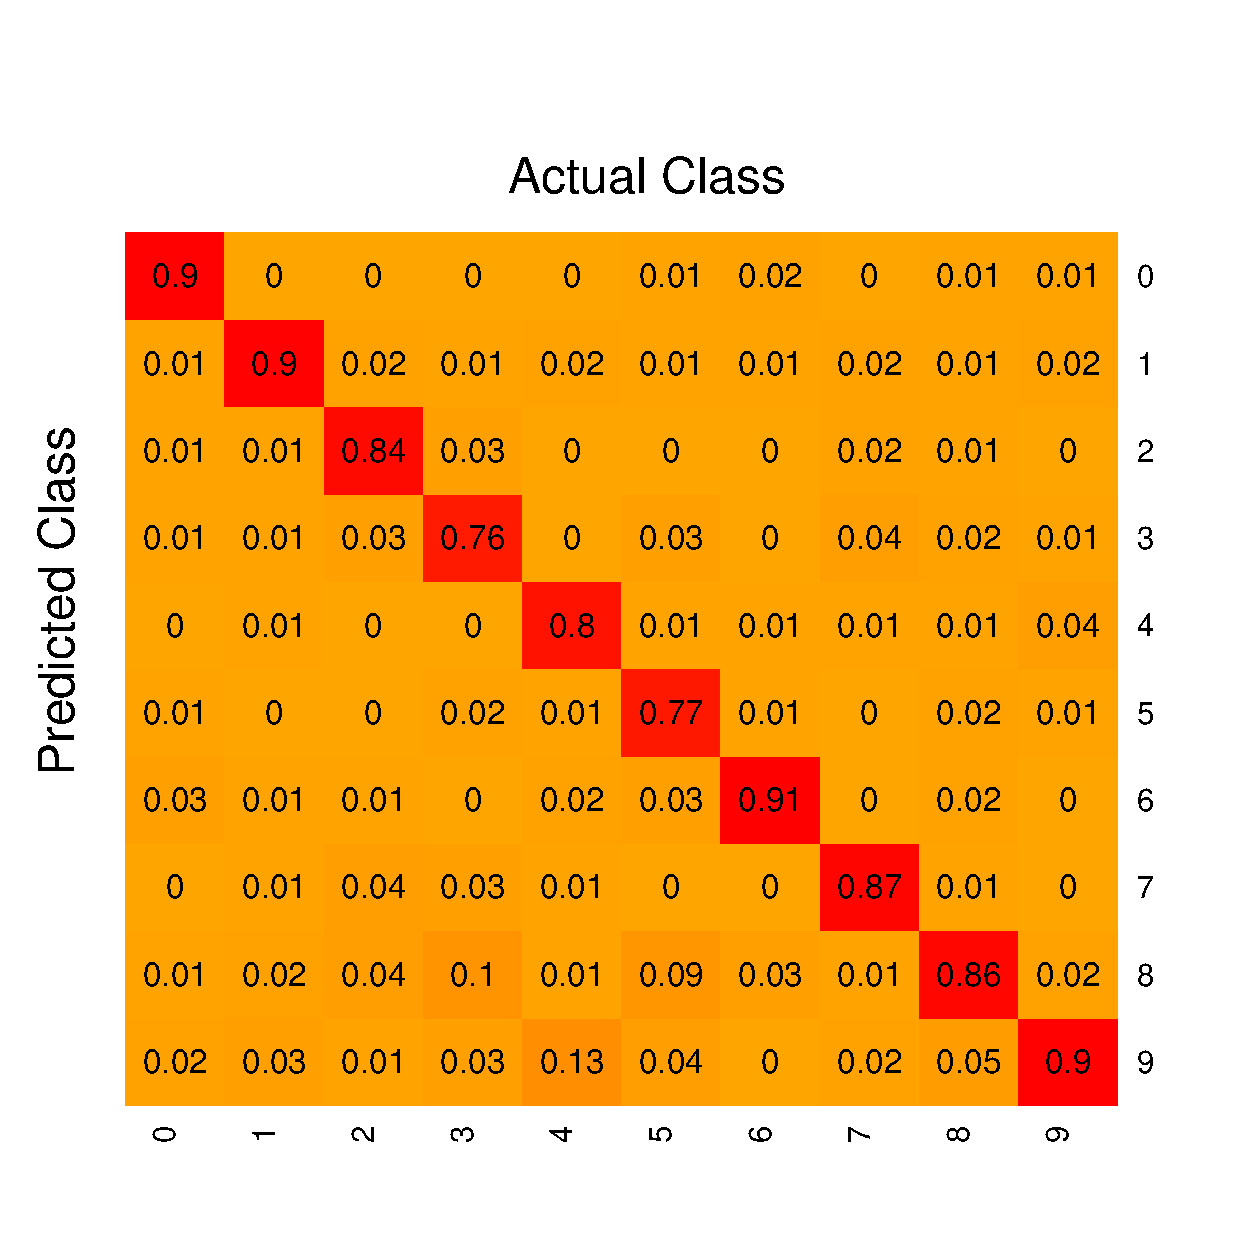
\includegraphics[width = 0.65 \textwidth]{graphics/knn_confusion_bestparam_easy}
\caption[Confusion table for the easy problem.]{Confusion table of the best parameter setting, for the easy problem with ten cross referencing runs.}
\label{fig:knn_conf_final_easy}
\end{figure}


\begin{figure}[H]
\centering
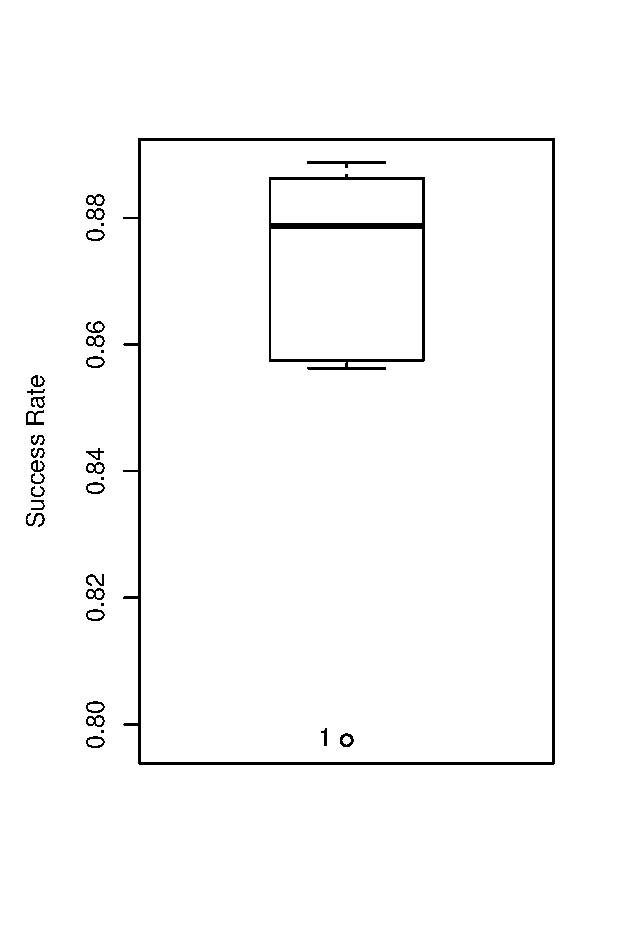
\includegraphics[width = 0.9 \textwidth]{graphics/knn_final_full_easy}
\caption[Success of K-NN on the easy problem.]{Success for the easy problem using ten cross referencing runs.}
\label{fig:knn_succ_final_easy}
\end{figure}


The hard problem is the one in which one persons test data was used as the test data alone and the remaining peoples put together in the training set.
This was done for all people with all the data present, such that each person once was used as the test set.
The success of such a process is seen in figure \ref{fig:knn_succ_final_hard} and figure \ref{fig:knn_conf_final_hard} shows the overall confusion table, when the confusion tables of each run was put together.


\begin{figure}[H]
\centering
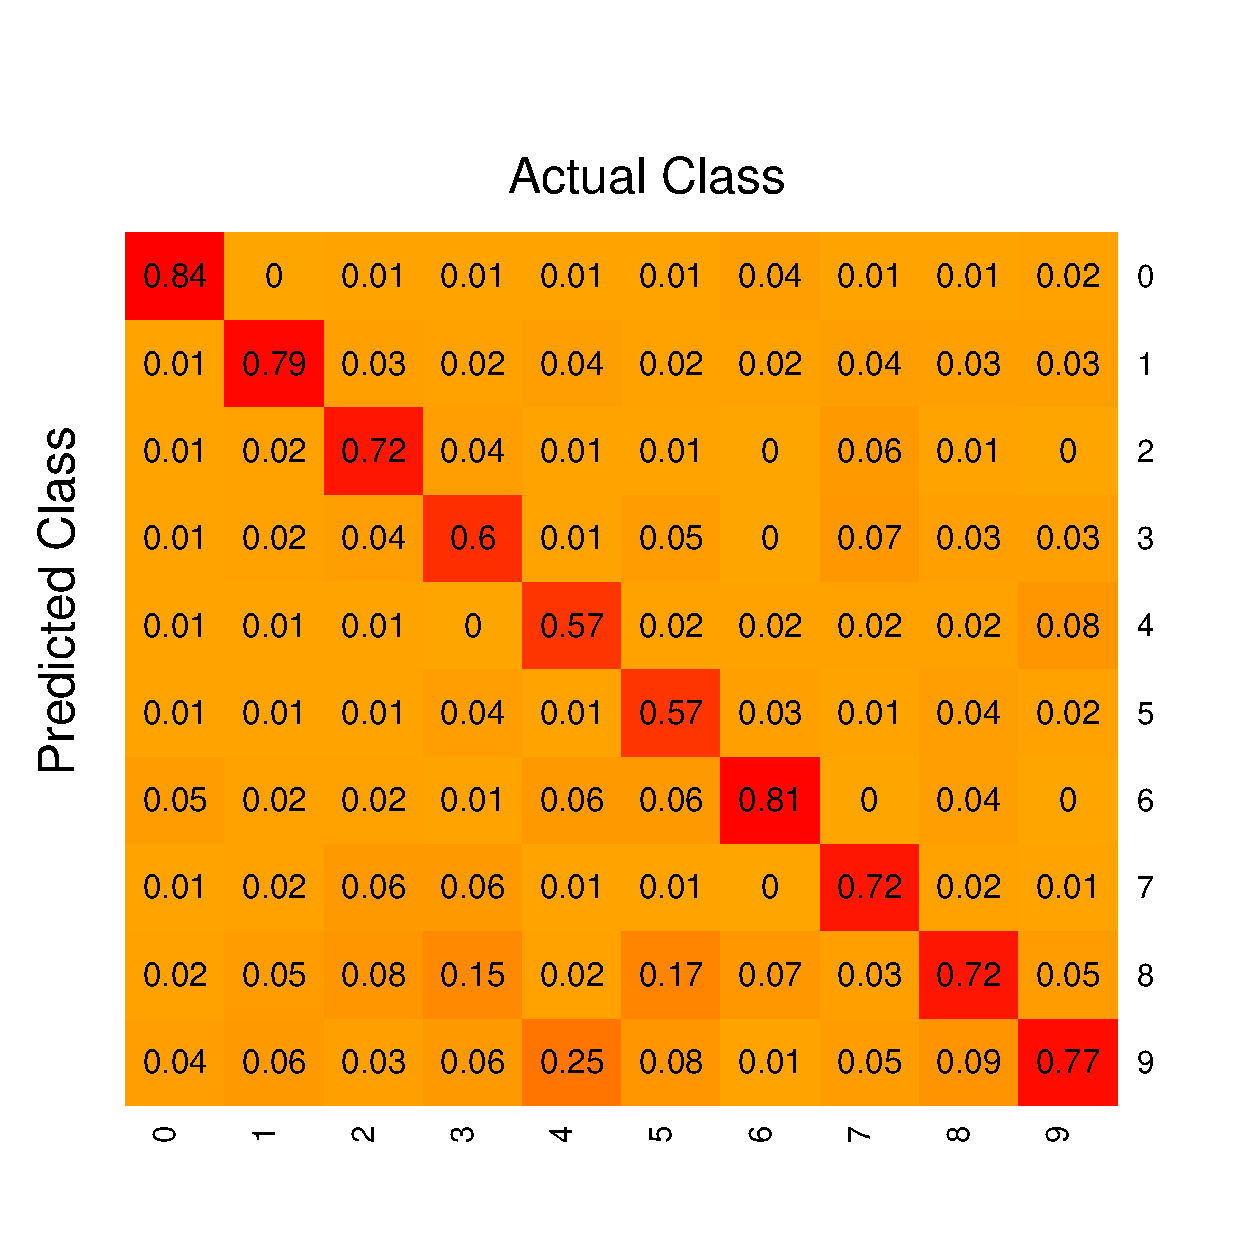
\includegraphics[width = 0.65 \textwidth]{graphics/knn_confusion_bestparam_hard}
\caption[Confusion table for the hard problem.]{Confusion table with all the best parameters for the full dataset difficult problem with the confusion tables for the different runs combined.}
\label{fig:knn_conf_final_hard}
\end{figure}


\begin{figure}[H]
\centering
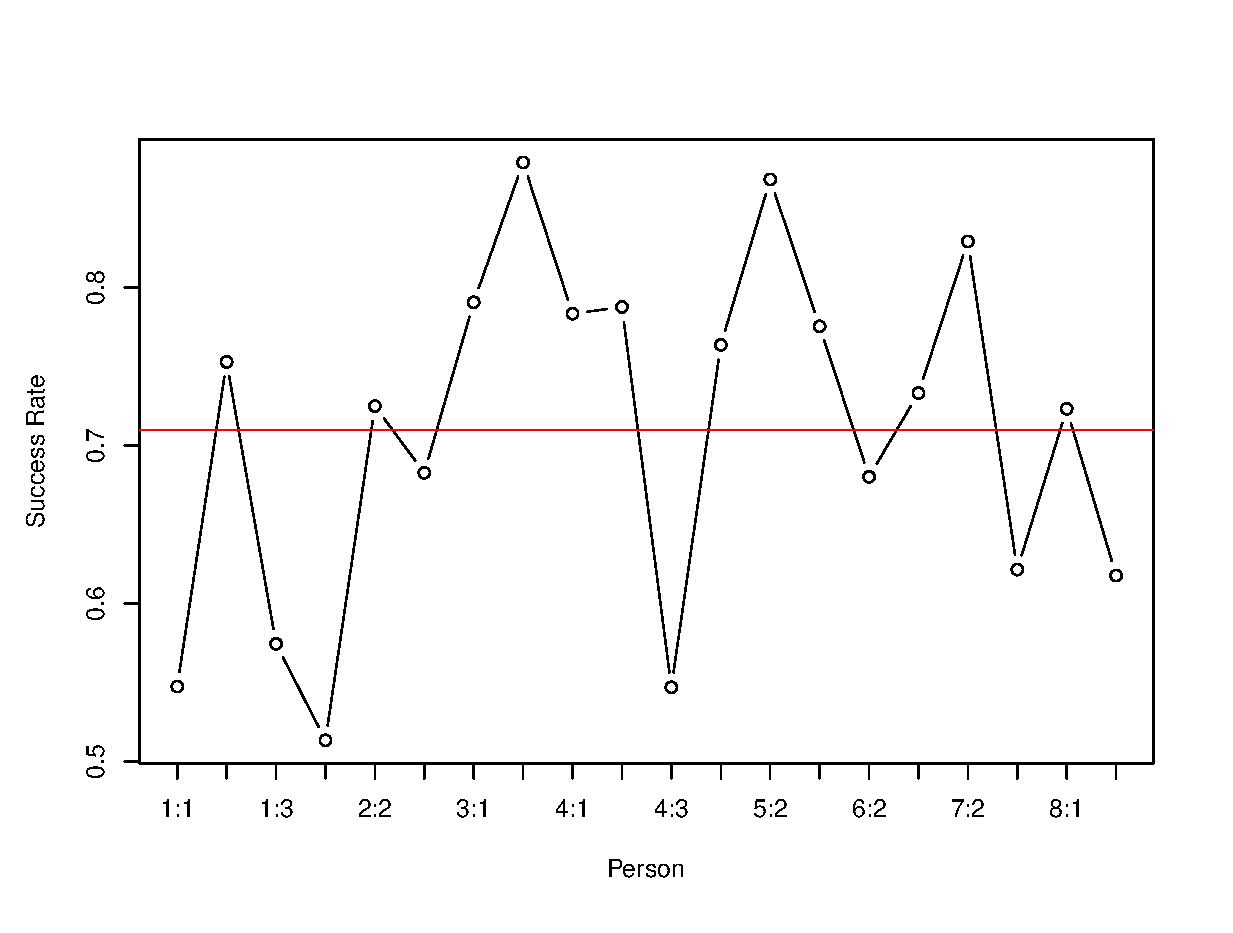
\includegraphics[width = 0.95 \textwidth]{graphics/knn_final_full_hard}
\caption[Success for K-NN for the hard problem.]{Success for the hard problem for each person.
The y-axis values represents the "Group:Member" number used as the test set.}
\label{fig:knn_succ_final_hard}
\end{figure}

With a mean of $70.99\%$ and variance of  $117.81\%^2$, then the hard problem clearly performs worse than the easy problem with $85.07\%$ mean and $3.59\%^2$ variance.
The general tendency is that the greatest error comes from the '3' and '5' often being detected as '8', and the '4' being classified as a '9'.
These two errors account for 5.7\% and 3.3\% of the error in hard and easy problem respectively, and is hence more than 1/6 in the two classification problems.
This is, however, expected as the characters of confusion have great similarity compared to any other class in the dataset.


\subsection{Conclusion}
It can be found that the optimal preprossing of the data for decision trees is
smoothing, then
z-score, then
PCA with 130 chosen components,
Boosting with 7 trials, and removal of leaves with less than 7 digits.

G2M1
has been found to have the worst handwriting when comparing the data of all people.




\newpage
\section{Algorithm Comparison}
\section{Introduction}
The classification of handwritten characters is used in a wide range of products to day.
Hence, this report goes in depth with how the numbers from zero to nine can be classified using machine learning algorithms.

The dataset consists of a set of handwritten characters from zero to nine.
These were constructed by the students enrolled in the course Statistical Machine learning (RM-SML-E1) of the year 2015 at the University of Southern Denmark (SDU).
The set used in this report is the 100DPI dataset.
Each number is hence stored as a $20px \times 20px$ matrix containing the handwritten character.

The methods used for classification are K-Nearest Neighbours and Decision Trees and Random Forests.
Furthermore a set of different ways to pre-process the data is explored.
Finally the two methods are compared with each at the best parameters and preprocessing settings.






\section{Conclusion}

\subsection{Worst Handwriting}


\newpage


% \section{K-Nearest Neighbours}
% 
% % % % Part one
% \subsection{Theory}
The K-Nearest Neighbour (K-NN) method is in this report used to classify a unknown digit to a set of known digits ranging from zero to nine.
%The data is split into two groups: One is for training and one is for testing. 
A set of the $k$ nearest neighbour is found using the euclidean distance to the pixel values in a training set of which the elements are already classified.
The result from the classification is found by counting the number of occurrences from the set of the $k$ nearest neighbours and choosing the most prominent.

%To see how this method performs a multitude of tests are performed to see how multiple parameters affect the success rate and the speed.

An example of such is seen in figure \ref{fig:knn_illustration}.

\begin{figure}[H]
\centering
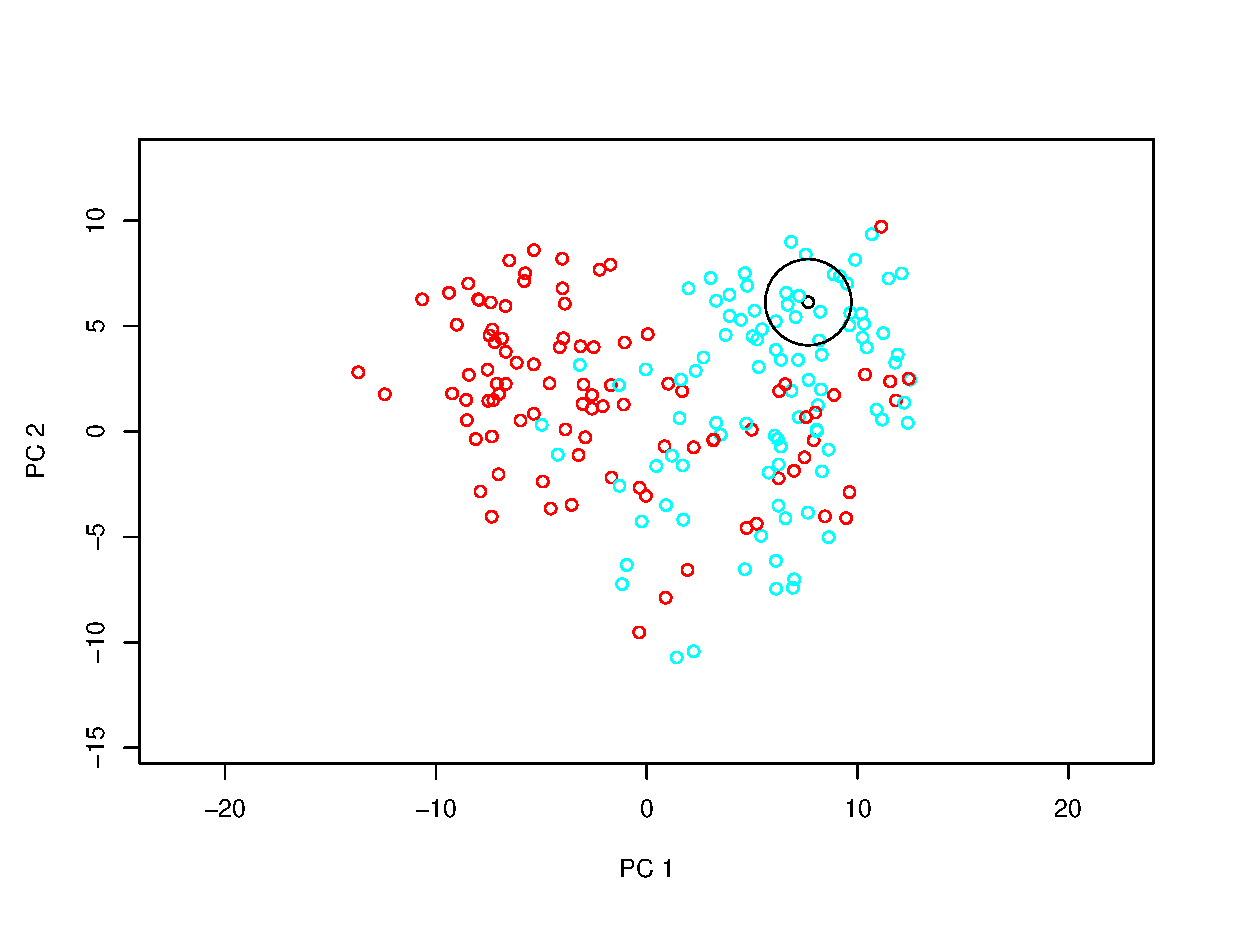
\includegraphics[width = 0.8 \textwidth]{graphics/knn_vis}
\caption[Illustration of the K-NN approach.]{Illustration of the K-NN approach with $k = 10$ on the normalized data for two classes plotting the two most prominent principle components.}
\label{fig:knn_illustration}
\end{figure}

In figure \ref{fig:knn_illustration} the black data point is an element of the blue test set.
The circle around it encircles the ten nearest neighbours.
Since there are more blue neighbours within the circle than red, then the classification in this case correctly classifies the element to the blue one.

\todo[inline]{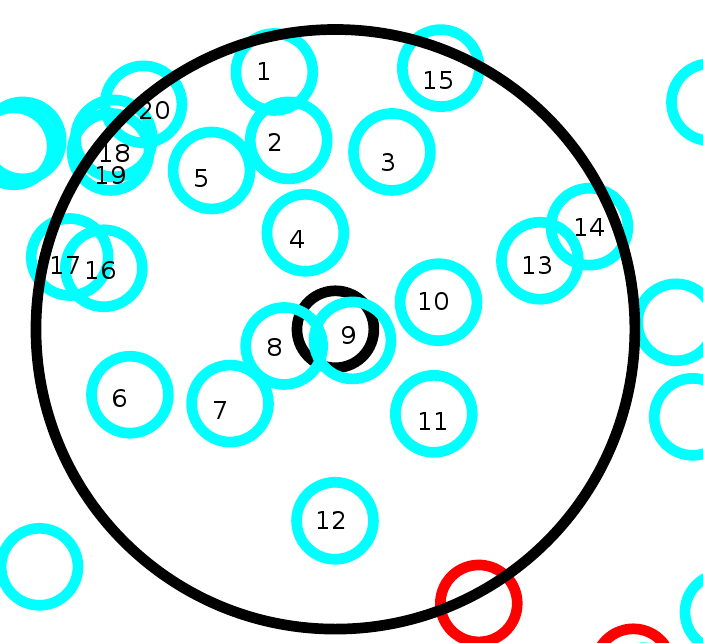
\includegraphics[width=0.2\textwidth]{graphics/knn_circle} Kan vi lave en cirkel om de 10 nærmeste?}
% 
% % \subsection{K-NN Implementation}


\lstinputlisting[language = R,
firstnumber = 291,
firstline = 291, 
lastline = 311, 
captionpos=b,
caption = {K-NN implementation.}]{../Code/KNN/01/test.R}
% 
% %1.5.1
%50/50, k = 10 -> tid vs DPI!
%confusion matrix på 1 run (100, 200 og 300 DPI) 
%1.5.2
%k vs Train Size (10 runs)
%1.5.3
%cross val. 10 runs 90/10 -> mean + var


\subsection{Single Person Tests}
This section tests the K-NN algorithm using data from one single person, namely Group three member two's data.
%
%The tests are performed first with the data split equally into a 50\% for the training and 50\% for the test set and the runtime is measured and compared for the three different image qualities. 
%
%Then test are performed with changing values of k and the training set size.
%
%Afterwards with a 90/10\% split for training and test respectively is computed and mean and variance is given.
%
%All the tests will be conducted using cross validation with 10 runs.

\subsubsection{Equally Sized training and test set}
To test the algorithm the data from the three different DPI's where split 50/50\% into a training and test set. 
The time to compute the test set for each DPI was then recorded and plotted. This is seen in figure \ref{fig:PersonDependent_5050}.
As expected does this scale with number of pixels. 

% % % % generated by timing.R
\begin{figure}[h]
\centering
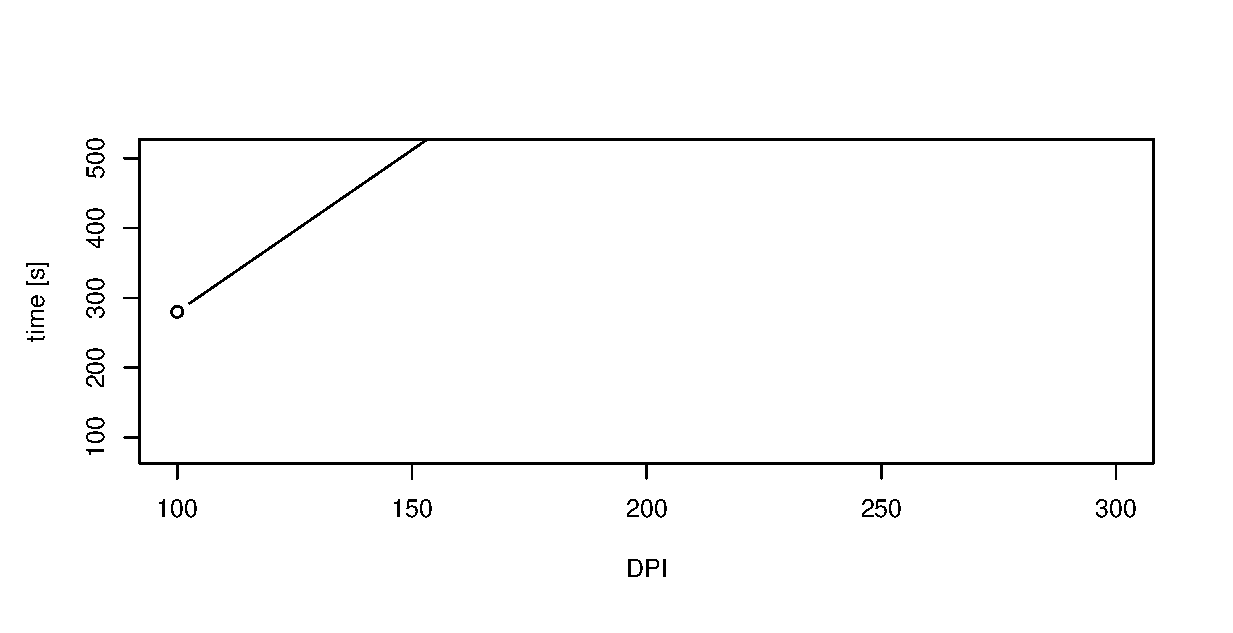
\includegraphics[width=\textwidth]{graphics/time_vs_dpi}
\caption{Timing of running a result with a 50/50\% split of group three member two's data}
\label{fig:PersonDependent_5050}
\end{figure}

Running the three test sets resulted in the confusion matrices seen in table \ref{tb:confus}.
They are all tested with a K of 10 and a split of 50/50\%.
In these it is seen which numbers do well and which numbers are hard to detect and which number they are detected as.
While the chance of matching a 1 with a 1 is really high there seem to be a high chance of getting a false positive as only 200 out of the 440 detected ones actually were correct.
And while the overall detection is good, the 8 is hard to detect with only 57\% success rate on 300 dpi.

% % % % generated by confusion.R
\begin{table}
    \centering
    \begin{subtable}{0.5\textwidth}
        \flushright
        
\begin{tikzpicture}
            \node at (0,0) {};
            \node at (1,0) {\huge Correct number}; 
        \end{tikzpicture}
    \end{subtable}

    \begin{subtable}{0.1\textwidth}
        \flushright
        
\begin{tikzpicture}
            \node[rotate=90] {\huge Guessed number};
        \end{tikzpicture}
    \end{subtable}
    \begin{subtable}{0.6\textwidth}
        \begin{subtable}{\textwidth}
            \centering
            {\scriptsize
                \begin{tabular}{l|*{10}{c}}
                    &0	& 1	& 2	& 3	& 4	& 5	& 6	& 7	& 8	& 9 \\
\hline
0	& 172	& 0	& 0	& 0	& 2	& 2	& 5	& 0	& 0	& 0 \\
1	& 18	& 199	& 24	& 21	& 30	& 26	& 25	& 19	& 32	& 57 \\
2	& 2	& 0	& 147	& 3	& 1	& 3	& 2	& 3	& 4	& 1 \\
3	& 5	& 1	& 14	& 172	& 0	& 6	& 18	& 6	& 34	& 14 \\
4	& 0	& 0	& 0	& 0	& 159	& 4	& 1	& 2	& 1	& 20 \\
5	& 0	& 0	& 0	& 0	& 0	& 154	& 0	& 0	& 2	& 0 \\
6	& 1	& 0	& 0	& 1	& 0	& 1	& 149	& 0	& 1	& 0 \\
7	& 0	& 0	& 10	& 2	& 0	& 0	& 0	& 169	& 0	& 1 \\
8	& 0	& 0	& 4	& 0	& 0	& 4	& 0	& 1	& 106	& 5 \\
9	& 2	& 0	& 1	& 1	& 8	& 0	& 0	& 0	& 20	& 102 \\

                \end{tabular}
            }
            \caption{Results for 100 DPI}
        \end{subtable}
        \begin{subtable}{\textwidth}
            \centering
            {\scriptsize
                \begin{tabular}{l|*{10}{c}}
                    &0	& 1	& 2	& 3	& 4	& 5	& 6	& 7	& 8	& 9 \\
\hline
0	& 172	& 0	& 0	& 0	& 1	& 3	& 0	& 0	& 1	& 1 \\
1	& 26	& 200	& 18	& 37	& 23	& 11	& 24	& 16	& 39	& 58 \\
2	& 0	& 0	& 160	& 2	& 0	& 1	& 4	& 0	& 2	& 0 \\
3	& 0	& 0	& 7	& 155	& 0	& 1	& 20	& 1	& 20	& 16 \\
4	& 0	& 0	& 0	& 0	& 168	& 1	& 0	& 1	& 0	& 6 \\
5	& 0	& 0	& 0	& 0	& 0	& 181	& 1	& 0	& 1	& 0 \\
6	& 2	& 0	& 0	& 0	& 1	& 0	& 150	& 0	& 4	& 0 \\
7	& 0	& 0	& 13	& 5	& 0	& 0	& 1	& 182	& 1	& 2 \\
8	& 0	& 0	& 1	& 0	& 0	& 1	& 0	& 0	& 103	& 1 \\
9	& 0	& 0	& 1	& 1	& 7	& 1	& 0	& 0	& 29	& 116 \\

                \end{tabular}
            }
            \caption{Results for 200 DPI}
        \end{subtable}
        \begin{subtable}{\textwidth}
            \centering
            {\scriptsize
                \begin{tabular}{l|*{10}{c}}
                    &0	& 1	& 2	& 3	& 4	& 5	& 6	& 7	& 8	& 9 \\
\hline
0	& 157	& 0	& 0	& 0	& 1	& 4	& 2	& 0	& 0	& 0 \\
1	& 37	& 200	& 24	& 33	& 17	& 14	& 18	& 19	& 30	& 48 \\
2	& 1	& 0	& 160	& 0	& 0	& 0	& 2	& 0	& 2	& 0 \\
3	& 1	& 0	& 1	& 152	& 0	& 0	& 7	& 1	& 15	& 9 \\
4	& 0	& 0	& 0	& 0	& 179	& 0	& 0	& 0	& 2	& 5 \\
5	& 0	& 0	& 0	& 0	& 1	& 181	& 0	& 0	& 1	& 0 \\
6	& 4	& 0	& 0	& 0	& 1	& 0	& 162	& 0	& 2	& 0 \\
7	& 0	& 0	& 15	& 15	& 0	& 0	& 9	& 180	& 3	& 2 \\
8	& 0	& 0	& 0	& 0	& 0	& 1	& 0	& 0	& 114	& 0 \\
9	& 0	& 0	& 0	& 0	& 1	& 0	& 0	& 0	& 31	& 136 \\

                \end{tabular}
            }
            \caption{Results for 300 DPI}
        \end{subtable}
    \end{subtable}
    \caption{Confusion matrices with different scaling}
    \label{tb:confus}
\end{table}

\subsubsection{Changing K and Training Set Size}
Tests was performed to see how both the value of K and size of the training set affects the accuracy of the K-NN algorithm. 
The result is given in figure \ref{fig:personDependent_contour}.

% \begin{figure}[H]
% \centering
% 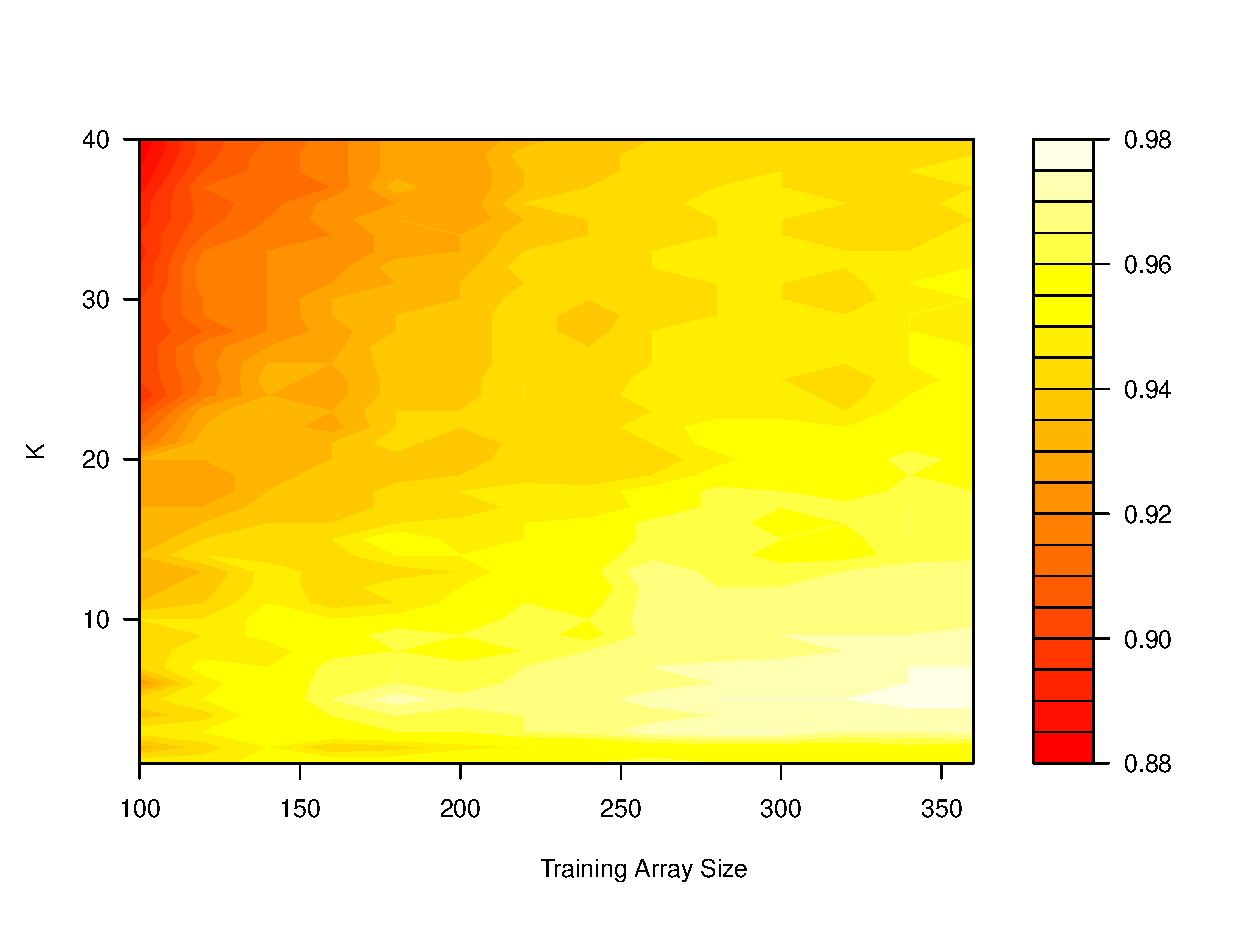
\includegraphics[width = 13cm]{graphics/graph_G3M2_20}
% \caption{Success Rate of the K-NN algorithm for changing values of K and the training set size.}
% \label{fig:personDependent_contour}
% \end{figure}

\begin{figure}[H]
\centering
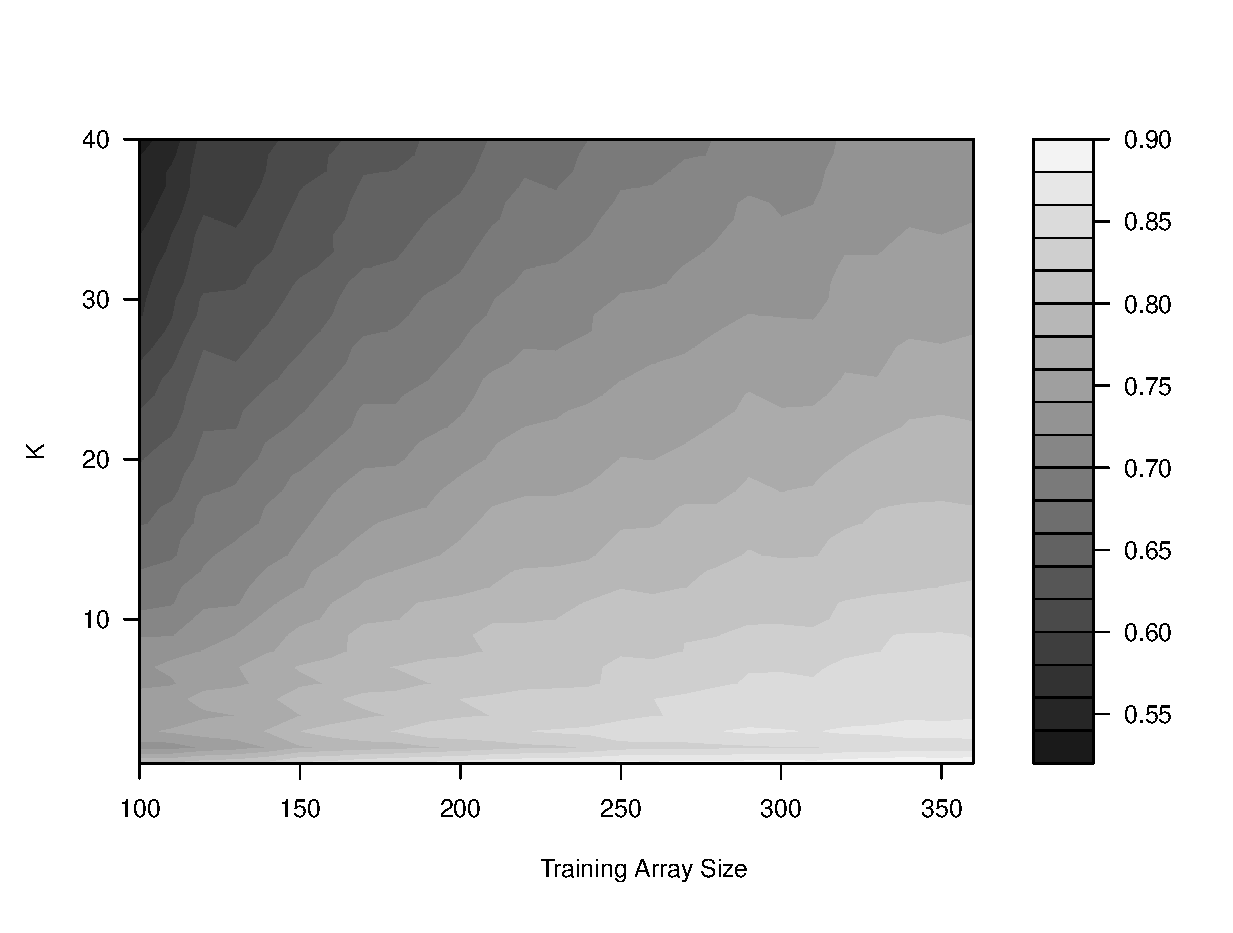
\includegraphics[width = 13cm]{graphics/graph_G3M2_10_10}
\caption{Success Rate of the K-NN algorithm for changing values of K and the training set size.}
\label{fig:personDependent_contour}
\end{figure}

% \begin{figure}[H]
% \centering
% 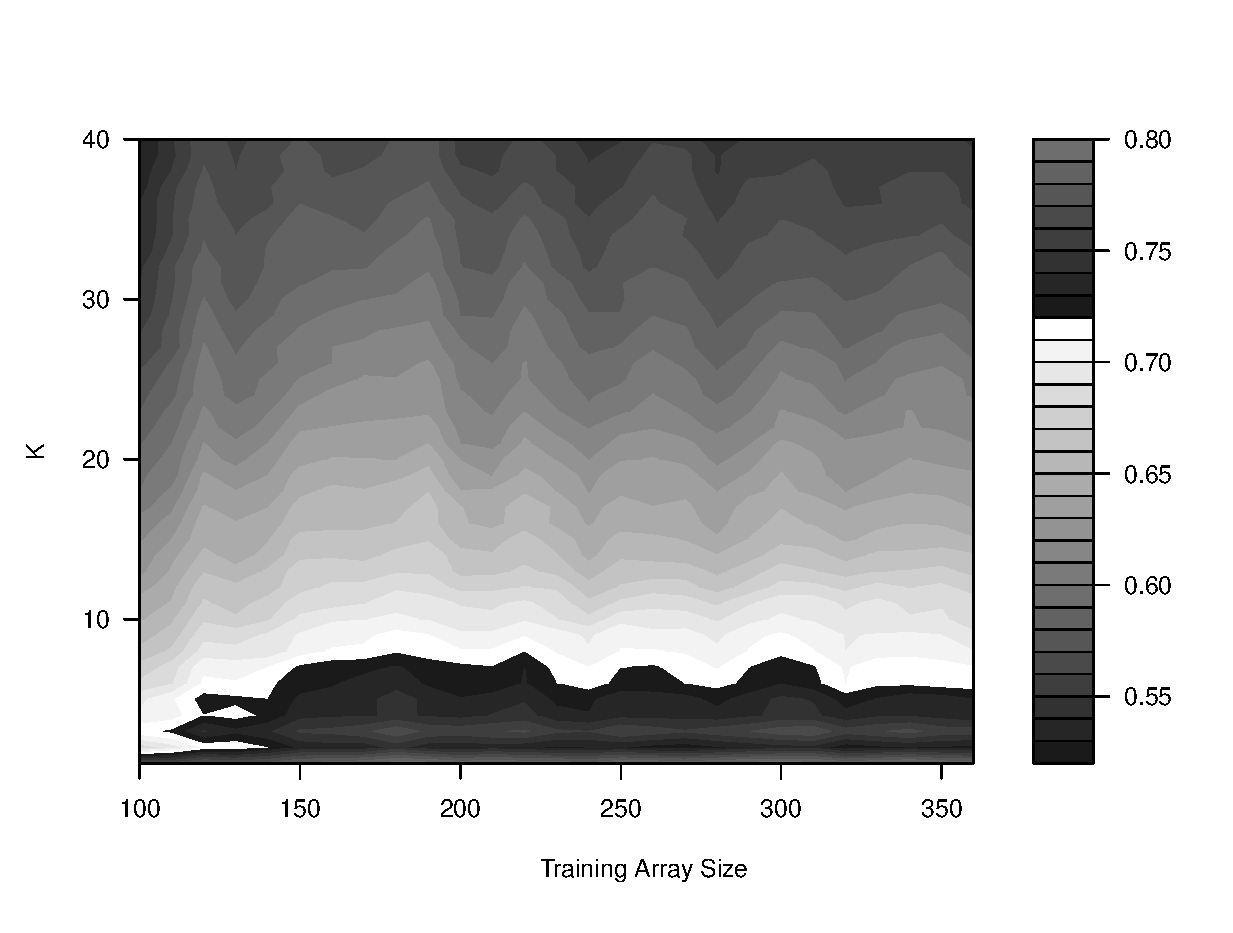
\includegraphics[width = 13cm]{graphics/graph_G3M1_10_10}
% \caption{Success Rate of the K-NN algorithm for changing values of K and the training set size.}
% \label{fig:personDependent_contour}
% \end{figure}

The test conducted in figure \ref{fig:personDependent_contour} where done with a test size of 40 and run 10 times with cross validation.

As seen on figure \ref{fig:personDependent_contour}, then the accuracy of the algorithm appears to increase as the train set size increases.
Furthermore the optimal value of K is dependent on the size of training set. 
As the size of the training set increases, so does the area where a the best performance is obtained.
From figure \ref{fig:personDependent_contour} it can be seen that the results are best when using a training size which is above 300 and K ranging between 3 and 7.


\subsubsection{90/10 Data Split}
A cross validation was also carried out using a 90/10\% and 50/50\% split of the data. 
Each test was made on both group members to see the difference.
The result of this is seen in figure \ref{fig:PersonDependent_9010}.
The values can be seen in \ref{tb:cross}

% % % % Generating this with cross_test.R tonight
\begin{figure}[h]
\centering
% 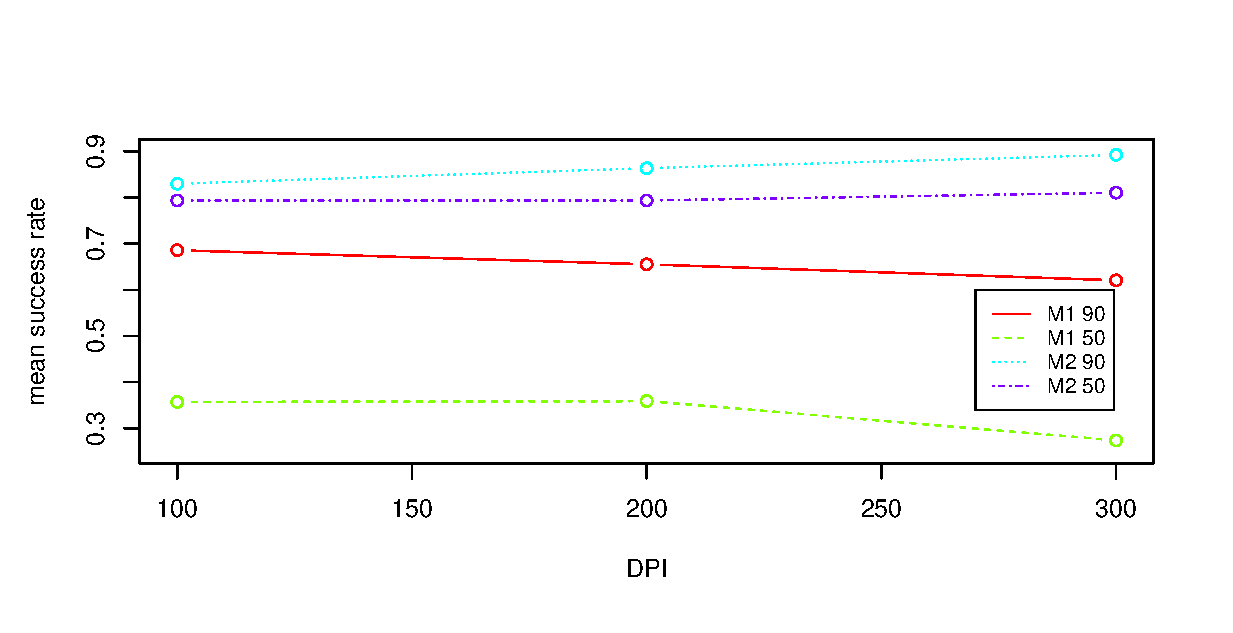
\includegraphics[width=\textwidth]{graphics/cross_test}
\caption[Cross validation]{Test result with a 90/10\% and 50/50\% split. The data points are taken as the mean of 10 runs using cross validation.}
\label{fig:PersonDependent_9010}
\end{figure}

\begin{table}[h]
\centering
    \begin{subtable}[b]{0.56\textwidth}
    \centering
        \begin{tabular}{lcccccc}
%             &M1 90	& M1 50	& M2 90	& M2 50 \\
\hline
100	& 0.6857	& 0.3570	& 0.8297	& 0.7935 \\
200	& 0.6552	& 0.3590	& 0.8635	& 0.7935 \\
300	& 0.6205	& 0.2735	& 0.8925	& 0.8105 \\

        \end{tabular}
        \caption{Mean success rate}
    \end{subtable}
    \begin{subtable}[b]{0.42\textwidth}
    \centering
        \begin{tabular}{lcccccc}
%             &M1 90	& M1 50	& M2 90	& M2 50 \\
\hline
100	& 0.0261	& 0.0253	& 0.01193	& 0.0223 \\
200	& 0.0275	& 0.8602	& 0.01100	& 0.0223 \\
300	& 0.0399	& 0.0708	& 0.00552	& 0.0154 \\

        \end{tabular}
        \caption{Variance in success rate}
    \end{subtable}
    \caption[Success of functions]{Success mean and variance of different split and data sets.}
    \label{tb:cross}
\end{table}




% 
% % 1.6.2: tabel over mean+var over 10 runs + 
%        graf dpi vs success for filtre (10 run)

\subsection{Preprocessed Image - Single Person Tests}

\begin{table}[h]
\centering
    \begin{subtable}[b]{0.56\textwidth}
    \centering
        \begin{tabular}{lcccccc}
            &Raw	& Avg	& G 0.5	& G 1	& G 2 \\
\hline
100	& 0.8297	& 0.860	& 0.8297	& 0.8545	& 0.7750 \\
200	& 0.8635	& 0.895	& 0.8635	& 0.8998	& 0.8602 \\
300	& 0.8925	& 0.920	& 0.8925	& 0.9190	& 0.8842 \\

        \end{tabular}
        \caption{Mean success rate.}
    \end{subtable}
    \begin{subtable}[b]{0.42\textwidth}
    \centering
        \begin{tabular}{lcccccc}
            &Raw	& Avg	& G 1	& G 2	& G 3 \\
\hline
100	& NA	& NA	& NA	& NA	& NA \\
200	& NA	& NA	& NA	& NA	& NA \\
300	& NA	& NA	& NA	& NA	& NA \\

        \end{tabular}
        \caption{Variance in success rate.}
    \end{subtable}
    \caption[Success of smoothing functions.]{Mean success rate and variance of different smoothing functions.}
    \label{tb:smooth}
\end{table}

\begin{figure}[h]
\centering
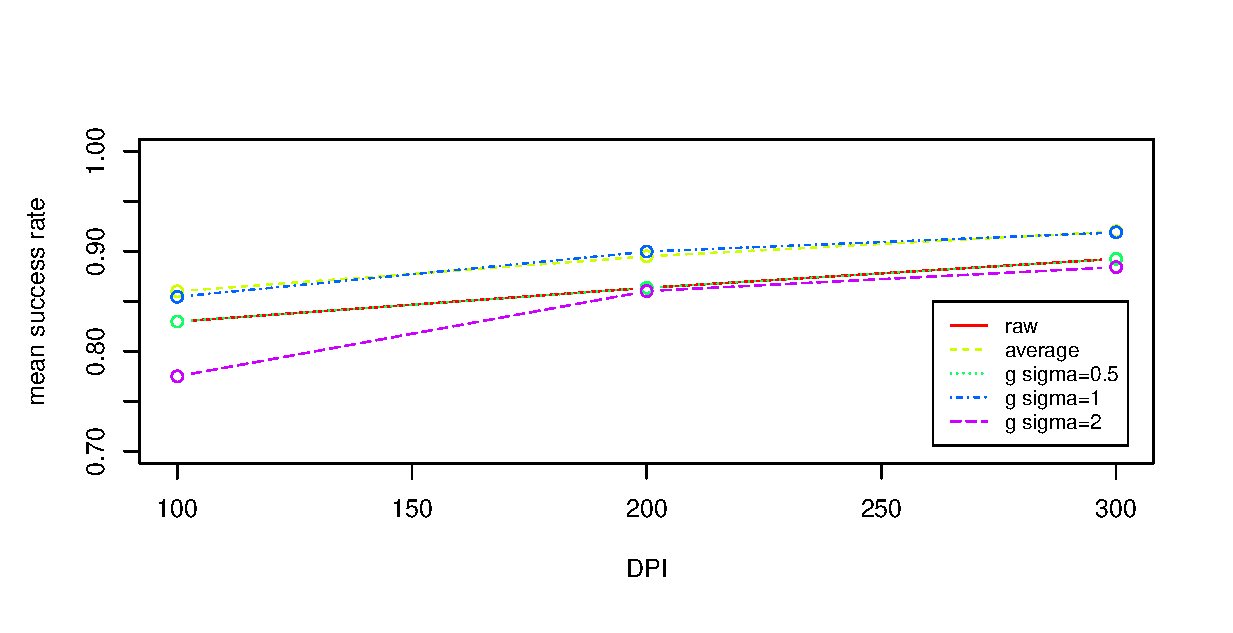
\includegraphics[width=1\textwidth]{graphics/smoothing}
\caption{Success rate of smoothing functions.}
\label{fig:smooth}
\end{figure}

Applying a smoothing function can give the image an advantage when using the nearest neighbour analysis.
By taking an average of the neighbouring pixels the lines in the digit should be wider and the digits should have a better chance of overlapping.
The danger is that too much smoothing could make the whole image one colour and would completely destroy any chance of analysis.
A Gaussian distribution (also referred to as a normal distribution) a naturally occurring distribution that happens when a random result occurs around a mean. 
The $\sigma$ signifies the deviation of the distribution. 
The 2D equation of a Gaussian distribution is shown in equation \ref{eq:gauss}. 

\begin{equation}
G(x,y) = \frac{1}{2\pi \sigma^2} e^{- \frac{x^2+y^2}{2\sigma^2}} \label{eq:gauss}
\end{equation}

Using the Gaussian filter to smooth an image will weigh the distance to the pixel.
A small $\sigma$ will make a small deviation and thus heavily weigh the center pixel.
The results of the filtering methods were also compared to the raw image with 100, 200 and 300 DPI.
These results are compared with an averaging filter (avg) which takes the average of the four neighbouring pixels and a Gaussian filter (G) with different values for sigma.
These tests were done 10 times, using cross validation, and the mean of each success rate is plotted in figure \ref{fig:smooth}. 
Since the variance is too small to be seen in the figure the mean and variance is shown in table \ref{tb:smooth}.
The averaging filter does not give a measurable different result from not using a filter.
The Gaussian filter does improves the success rate for some values of sigma, but a larger $\sigma$ makes it worse.

% 
% %\section{K-NN on Big Data}
% \section{Introduction}
The classification of handwritten characters is used in a wide range of products to day.
Hence, this report goes in depth with how the numbers from zero to nine can be classified using machine learning algorithms.

The dataset consists of a set of handwritten characters from zero to nine.
These were constructed by the students enrolled in the course Statistical Machine learning (RM-SML-E1) of the year 2015 at the University of Southern Denmark (SDU).
The set used in this report is the 100DPI dataset.
Each number is hence stored as a $20px \times 20px$ matrix containing the handwritten character.

The methods used for classification are K-Nearest Neighbours and Decision Trees and Random Forests.
Furthermore a set of different ways to pre-process the data is explored.
Finally the two methods are compared with each at the best parameters and preprocessing settings.




% %% % Part two
% \subsection{K-NN on Big Data}
% %
% \subsection{Principle Component Analysis}
A Principle Component Analysis (PCA) aims at reducing the number of dimension used to represent the features of the data.
This is done by finding the eigenvectors and eigenvalues to the training set and removing some of the components representing the least variance in the data set.
Thus efficiently reducing the dimensions, but still keeping the most significant knowledge about the features.

\begin{figure}[h]
\begin{subfigure}{0.49\textwidth}
\centering
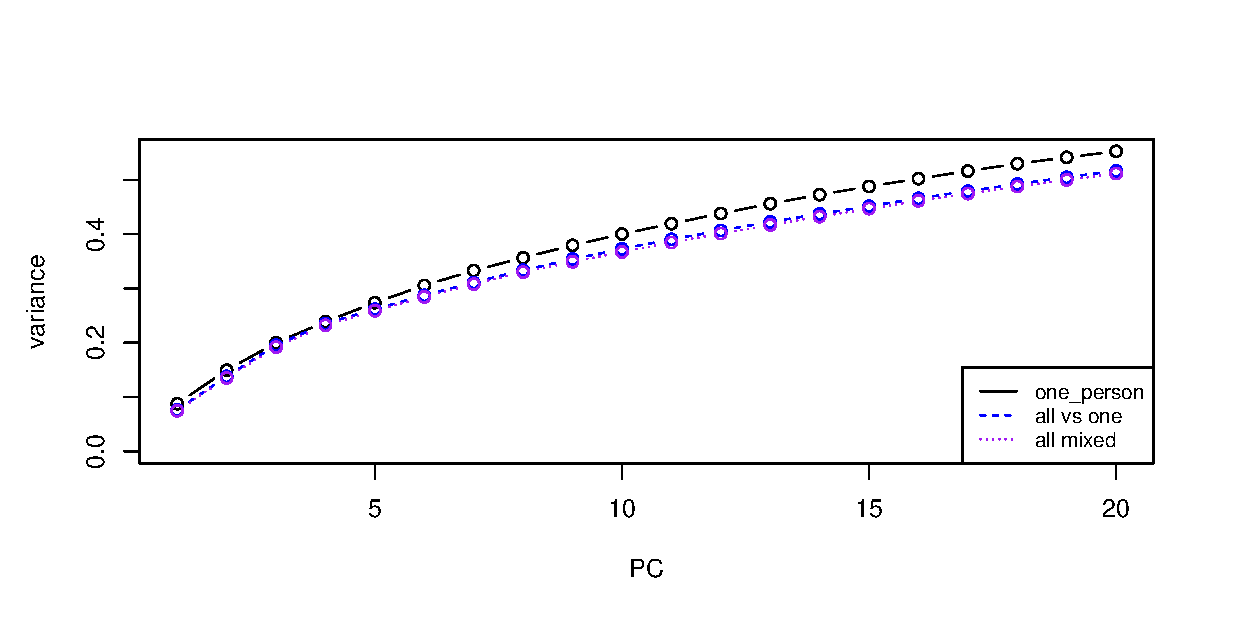
\includegraphics[width=\textwidth]{graphics/pca_acc_variance}
\caption{Accumulated variance}
\label{fig:pca_accumulated_var}
%
\end{subfigure}
\begin{subfigure}{0.49\textwidth}
\centering
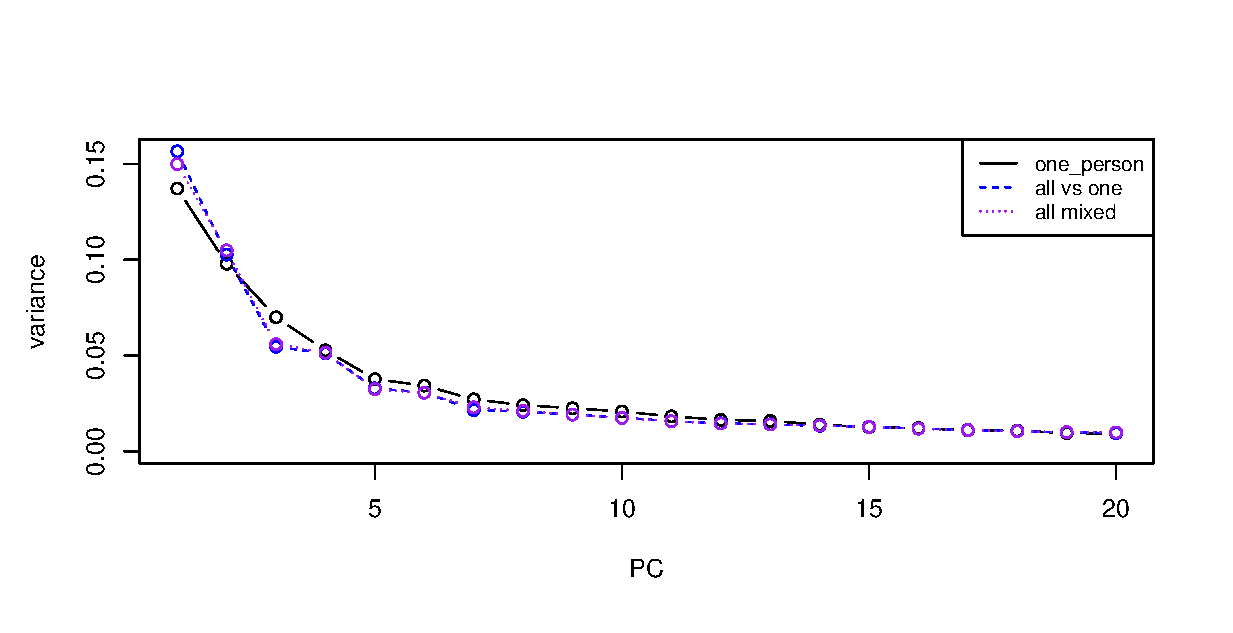
\includegraphics[width=\textwidth]{graphics/pca_variance}
\caption{Variance}
\label{fig:pca_accumulated_var}
\end{subfigure}
\caption[PCA variance]{Variance over the first 20 principle components.
The data was run on Group 3 member 1's data on 100 DPI. }
\label{fig:variance}
\end{figure}
% Figure \ref{fig:contour_KvsPCA_G3M2vsRest} shows a contour plot of how well Group 3 Member 2's  handwriting was predicted successfully for $K$ and the total variance represented of the PC's varying between one and 20 and 0.5 and 1 respectively.

The principle components analysis (PCA) is an tool that can be used to describe the variance in a data set.

By selecting the most significant principle components (PC) the data set can be systematically reduced with minimal changes to performance.
In figure \ref{fig:variance} is the variance and accumulated variance shown for the first 20 PC. 
It is seen that the first PC is the most significant and the variance converges towards zero with more PC.

Calculating with less data will result in a faster computation time. But it can be hard to predict if the performance becomes better or worse.
Choosing too few PC and there is no features left to compare.
To see how the performance and the timing scales both are shown in figure \ref{fig:pca_timing}. K was chosen to be 10.
The success rate has a peak with a low set of attributes so there must be some confusion that gets sorted out. 

\begin{figure}[h]
\centering
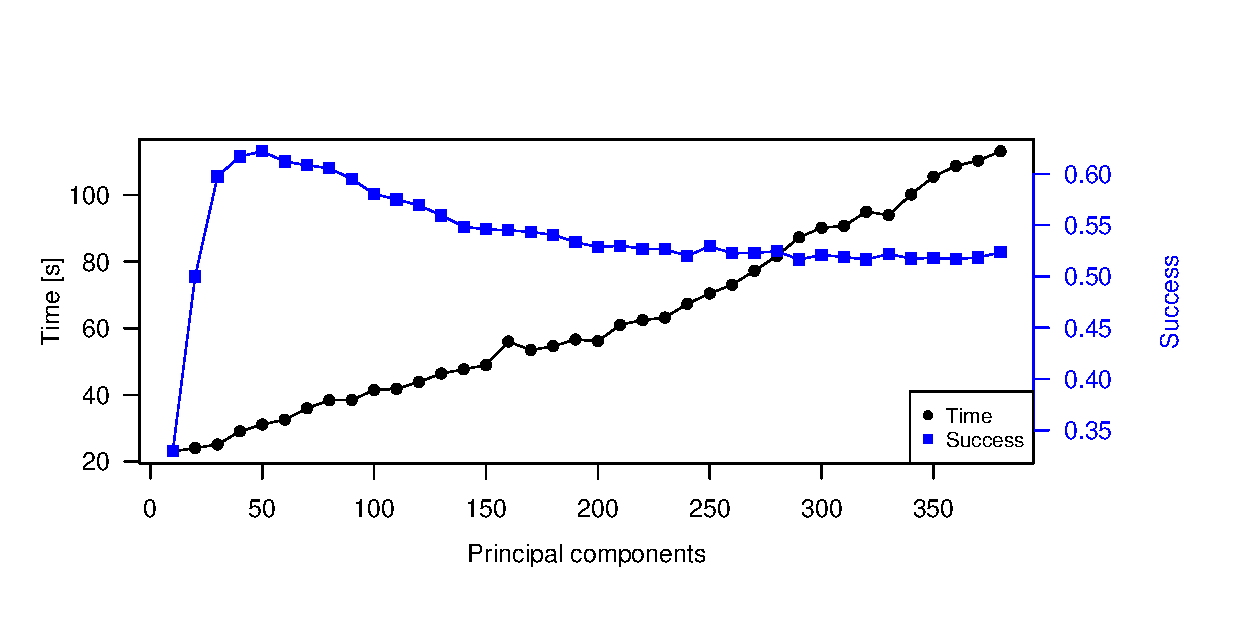
\includegraphics[width =0.8 \textwidth]{graphics/pca_timing_nikolaj}
\caption[Timing of PCA]{Timing of running the PCA with different principle components. 
The data was run on Group 3 member 1's data on 100 DPI. 
The percentage of successful predictions is also measured with the same data.}
\label{fig:pca_timing}
\end{figure}

As seen on figure \ref{fig:contour_KvsPCA_G3M2vsRest}, then the optimum K and represented PCA variance is at $K = 19$ and $PCA = 0.8$. 
This is because an as high successful prediction rate is wanted, but also an as small dataset as possible. 
This point will further be used in section \ref{sec:DataNormalization}.

To get a closer look at how the PCA performs the data from G3M2 was tested against the rest of the class. 
The K was chosen to be 10. 
The data is shown in figure \ref{fig:pca_success}.
The performance is getting worse as more features are considered.

\begin{figure}[h]
\centering
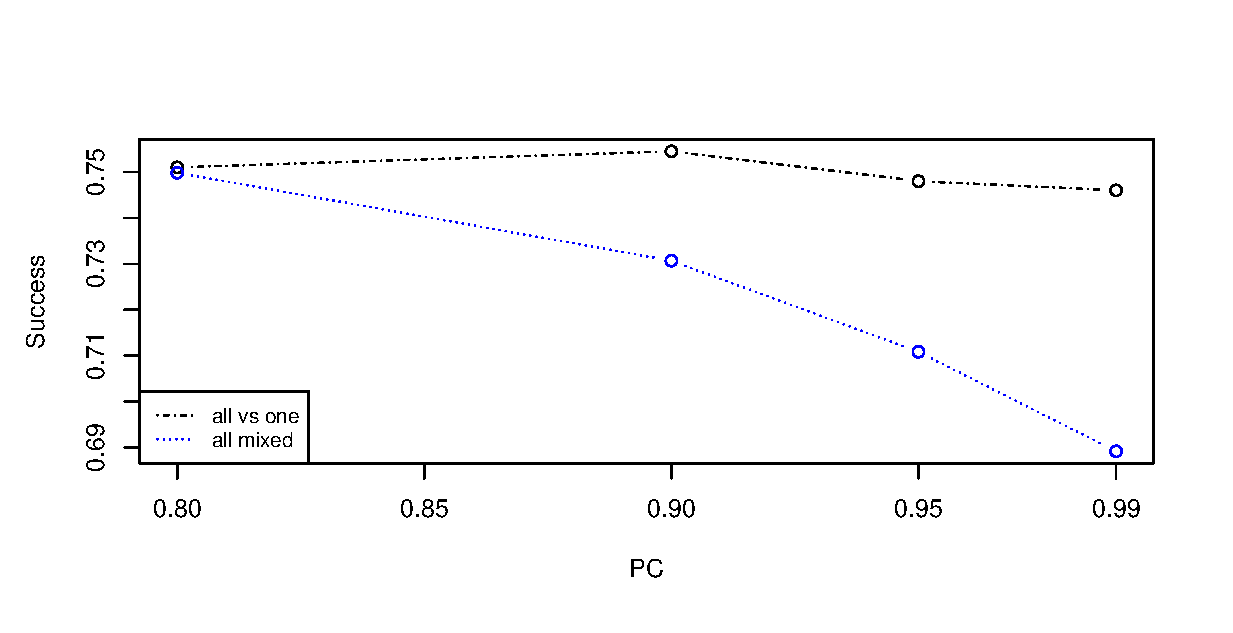
\includegraphics[width =0.8 \textwidth]{graphics/pca_success}
\caption[PCA performance]{Percentage of successful predictions with an increasing accumulated variance used.
The data was run on Group 3 member 2's vs data from 14 members on 100 DPI. }
\label{fig:pca_success}
\end{figure}

To investigate the impact of K the test was redone so more K's were tested and that would lead to finding an optimum K for the large data set.
The data is shown in figure \ref{fig:k_v_PCA}. 
Where the optimum K was very small when testing a single person, a larger K is better suited for tests involving large data sets.
there still seems to be an optimum data size where the full data set performs worse than a smaller data set. 

\begin{figure}[h]
\centering
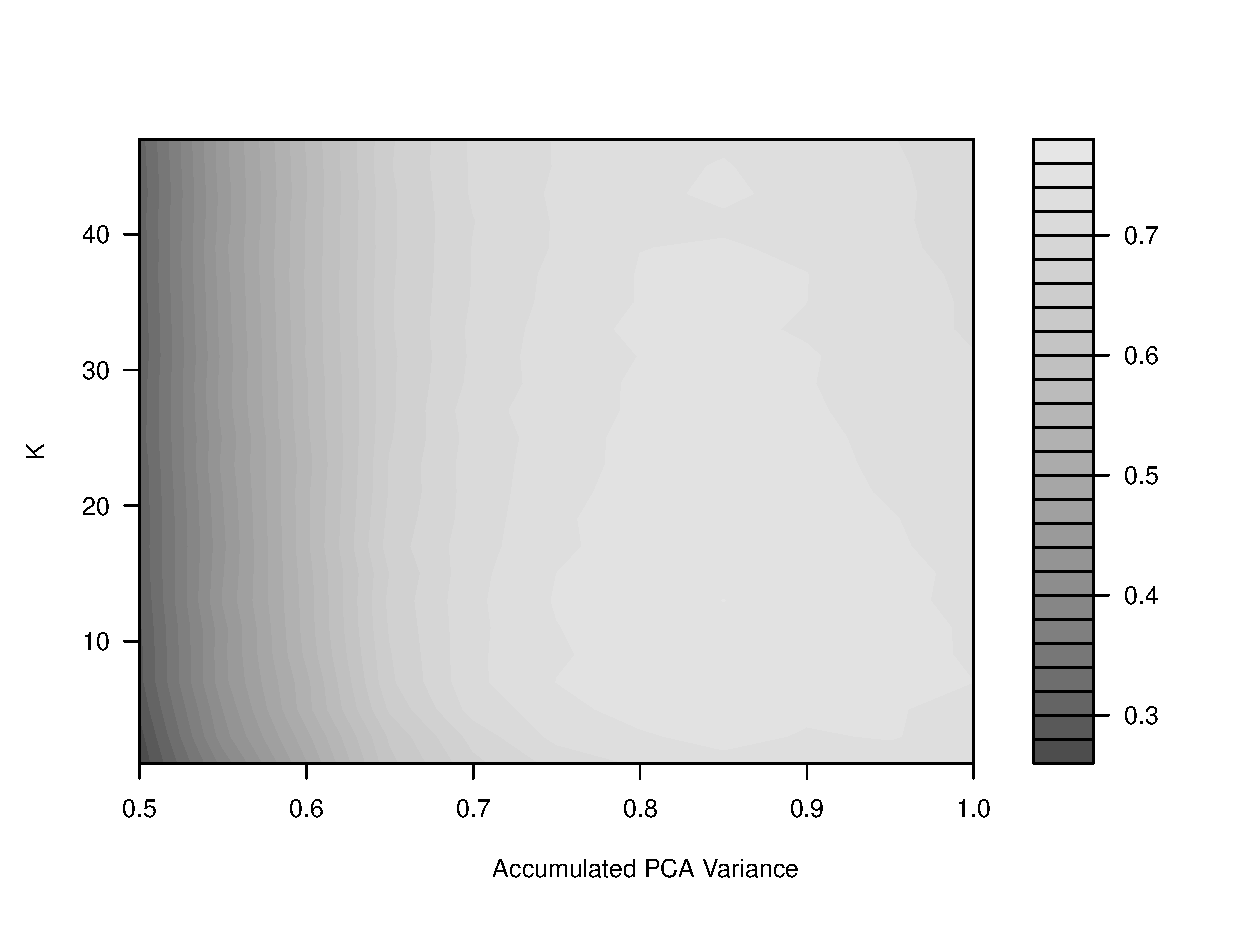
\includegraphics[width = \textwidth]{graphics/contour_k_PCA_oneVsRest}
\caption[Detailed PCA performance]{Success rate for detection of characters of Group 3 Member 2's data when he himself is not represented in the training set. 
The test was done with 16 people.}
\label{fig:k_v_PCA}
\end{figure}



% %
% \subsection{Data Normalization and Binning}

\begin{figure}[h]
\centering
    \begin{subfigure}{0.2\textwidth}
        \includegraphics[width = \textwidth]{graphics/bins_inf}
    \end{subfigure}
    \begin{subfigure}{0.2\textwidth}
        \includegraphics[width = \textwidth]{graphics/bins_10}
    \end{subfigure}
    \begin{subfigure}{0.2\textwidth}
        \includegraphics[width = \textwidth]{graphics/bins_5}
    \end{subfigure}
    \begin{subfigure}{0.2\textwidth}
        \includegraphics[width = \textwidth]{graphics/bins_2}
    \end{subfigure}
\caption{look at these beautiful 2's}
\end{figure}
% %
% \subsection{K-means}
K-means is used to group the data set into categories depending on their location in the x-dimensional space determined by the amount of features representing one of them.
The center of these clusters are then computed and identified as a specific category.
Using these centres, a unknown element can then be categorized depending on which cluster is the closest.

To find the number of clusters best representing the data set, then the within-group heterogeneity and homogeneity was computed for various K's as seen on figure \ref{fig:elbow_point}.
The elbow point can from here be determined to be at K of 1300 where it has 73.6\% homogeneity.

% It is also shown that normalizing the data or using a filter doesn't improve the performance. It actually hurts the performance. 

% k_means_elbow.R
\begin{figure}[H]
\centering
\begin{subfigure}{0.70\textwidth}
\centering
\includegraphics[width=\textwidth]{graphics/homogenity}
\caption{homogeneity}
\label{fig:homogeneity_kmean}
\end{subfigure}\\[-1cm]
\begin{subfigure}{0.70\textwidth}
\centering
\includegraphics[width=\textwidth]{graphics/heterogenity}
\caption{heterogeneity}
\label{fig:heterogeneity_kmean}
\end{subfigure}
\caption[K means elbow point]{homogeneity and heterogeneity of the data set.}
\label{fig:elbow_point}
\end{figure}


\begin{table}[H]
\centering
%# kmean = 1500
%# k_knn = 10
%# k_mean = 10     
%# kmean_iterations = 500
%# Time taken to prep kmean: 747.229999999996
%# Time taken to run kmean classification: 42.1600000000035
%# Success for kmean: 0.54275
%# Time taken to prep norm kmean: 802.549999999996
%# Time taken to run norm kmean classification: 44.4400000000023
%# Success for norm kmean: 0.63125
%# Time taken to run raw knn classification: 1878.1
%# Success for raw knn: 0.73625

\begin{tabular}{|l|p{2cm}|p{2cm}|p{2cm}|}\hline
Criteria              & None   & K-mean & Normalized K-mean \\ \hline
Pre-Processing Time*  & 0s     & 12m27s & 13m23s            \\ \hline
Classification Time** & 31m18s & 42.2s  & 44.4s             \\ \hline
Success Rate**        & 73.6\% & 54.3\% & 63.1\%            \\ \hline
\multicolumn{4}{|l|}{* of 60,000 elements} \\ 
\multicolumn{4}{|l|}{** of 4,000 elements} \\ \hline
\end{tabular}

% \begin{tabular}{|l|p{2cm}|p{2cm}|p{2cm}|}\hline
% Criteria              & None    & K-mean  & Normalized K-mean  \\ \hline
% Pre-Processing Time*  & 0s      & 14m3.3s & 15m7.7s            \\ \hline
% Classification Time** & 18m1.7s & 43.5s   & 39.6s              \\ \hline
% Success Rate**        & 73.7\%  & 54.1\%  & 60.4\%             \\ \hline
% \multicolumn{4}{|l|}{* of 60,000 elements} \\ 
% \multicolumn{4}{|l|}{** of 4,000 elements against the training set.} \\ \hline
% \end{tabular}
\caption{Processing time comparison of running K-NN on K-mean data, normalized + k-mean data and raw data. 
K-mean makes 1300 clusters and max 500 iterations, the K-NN algorithm is applied with k = 10.}
\label{tab:processingtime_kmean_vs_raw_knn}
\end{table}

As seen in table \ref{tab:processingtime_kmean_vs_raw_knn} K-means clustering reduces the processing time at the cost of performance. 
Depending on the data set and the hardware this should be taken into consideration. 
Because K-means is a random algorithm the timing is unpredictable. If the starting points are very good the timing will decrease. 
A way to force this behaviour is to set a max iteration that is low enough so the timing will always be low.
This will cause the random selection to affect the performance. 
If a high enough max iteration is selected the timing might be so bad that K-means clustering is not worth the reduction in successful classifications.

% \section{Decision Trees}

% \section{Introduction}
The classification of handwritten characters is used in a wide range of products to day.
Hence, this report goes in depth with how the numbers from zero to nine can be classified using machine learning algorithms.

The dataset consists of a set of handwritten characters from zero to nine.
These were constructed by the students enrolled in the course Statistical Machine learning (RM-SML-E1) of the year 2015 at the University of Southern Denmark (SDU).
The set used in this report is the 100DPI dataset.
Each number is hence stored as a $20px \times 20px$ matrix containing the handwritten character.

The methods used for classification are K-Nearest Neighbours and Decision Trees and Random Forests.
Furthermore a set of different ways to pre-process the data is explored.
Finally the two methods are compared with each at the best parameters and preprocessing settings.




% \subsection{Entropy}
To compute the optimum decision point for the individual principle components, the entropy method is used.
The entropy of the PC's with our ten ciphers is given by equation \ref{eq:entropy}.

\begin{equation}
Entropy(S) = \sum_{i = '0'}^{'9'} -p_i \cdot \log_2(p_i) 
\qquad \because p_i = P(x = i)
\label{eq:entropy}
\end{equation}

To find the best decision point, it is wished that the entropy of the two resulting systems, when dividing one PC into two, is as low as possible.
This can be represented as sum of entropy for our two resulting datasets, weighted by the relative size of such.
This is given in equation \ref{eq:entropy_datasetdevision}.

\begin{eqnarray}
Entropy = \sum_{i = 1}^{2} \frac{s_i \cdot Entropy(S_i)}{\sum_{k = 1}^{2} s_k} 
\qquad \because S_i \subset S\ and\ s_k = size(S_k)
\label{eq:entropy_datasetdevision}
\end{eqnarray}

When using equation \ref{eq:entropy_datasetdevision} on the first five principle components on the data of 15 people from the class, then figure \ref{fig:entropy_pc5} was gained.

\begin{figure}[H]
\centering
\includegraphics[width = 0.95 \textwidth]{graphics/entropy_pc}
\caption{Figure showing the variation of the entropy of the dataset when the decision point varies. Computed using equation \ref{eq:entropy_datasetdevision}. The data of the first five principle component.}
\label{fig:entropy_pc5}
\end{figure}


The point of lowest entropy for a principle component was then used as the splitting point to convert the data into binary.
This was done by setting everything below the splitting point to true and the rest false.
This was then done for all principle components on both the test and train set. 
The splitting point for the components in the test set were taken as the splitting point from the same component in the train set.

The optimal decision decision point is shown along with the PC values for PC1 in figure \ref{fig:decision_point}. 
Here it is clear that if the data is above the split then it can not be a 0.
If the data is below, further investigation is needed.
By removing all unlikely classes the true class must remain.

\begin{figure}[H]
\includegraphics[width = \textwidth]{graphics/decision_seperation}
\caption{Decision point in relation to PC values}
\label{fig:decision_point}
\end{figure}
% \subsection{Decision Trees}

The idea of a decision tree is to split the classifications into a set of decisions.
The first 50 PCA values are used and by looking at the deviance for each split a tree can be created.

\begin{figure}[h]
\includegraphics[width = \textwidth]{graphics/tree_section}
\caption{Small section of the tree}
\label{fig:tree_section}
\end{figure}

Building a tree can be done using the ``C50'' library in R.
The tree with the training data of 15 people (56000 cases) contains 6338 nodes.
A small section of the tree is shown in figure \ref{fig:tree_section}.
Each node shows which principal component and the split to which the decision is made.
Each leaf shows the probability of a classification.\\
The classifications is shown in table \ref{tb:tree_confus}.

\begin{table}[H]
    \centering
    \begin{subtable}{0.005\textwidth}
    \end{subtable}
    \begin{subtable}{0.8\textwidth}
        \centering
        
\begin{tikzpicture}
            \node at (0,0) {};
            \node at (1,0) {\Large Actual Class}; 
        \end{tikzpicture}
    \end{subtable}

    \begin{subtable}{0.005\textwidth}
        \flushright
        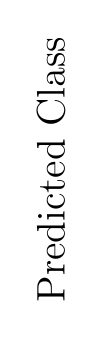
\begin{tikzpicture}
            \node[rotate=90] {\Large Predicted Class};
        \end{tikzpicture}
    \end{subtable}
    \begin{subtable}{0.8\textwidth}
        \begin{subtable}{\textwidth}
            \centering
            \begin{tabular}{*{11}{c}}
                &0	& 1	& 2	& 3	& 4	& 5	& 6	& 7	& 8	& 9 \\
\hline
0	& 348	& 1	& 0	& 0	& 3	& 4	& 7	& 2	& 2	& 2 \\
1	& 0	& 349	& 3	& 2	& 4	& 0	& 1	& 1	& 1	& 3 \\
2	& 2	& 2	& 347	& 3	& 3	& 2	& 1	& 2	& 2	& 1 \\
3	& 0	& 1	& 3	& 346	& 1	& 1	& 0	& 2	& 5	& 1 \\
4	& 2	& 0	& 1	& 0	& 338	& 8	& 0	& 2	& 1	& 0 \\
5	& 1	& 0	& 0	& 3	& 5	& 342	& 1	& 2	& 1	& 2 \\
6	& 3	& 6	& 0	& 0	& 1	& 1	& 348	& 2	& 3	& 3 \\
7	& 1	& 0	& 1	& 3	& 1	& 1	& 0	& 342	& 2	& 5 \\
8	& 2	& 0	& 3	& 2	& 0	& 1	& 1	& 3	& 338	& 5 \\
9	& 1	& 1	& 2	& 1	& 4	& 0	& 1	& 2	& 5	& 338 \\

            \end{tabular}
            \caption{Confusion table of decision tree}
            \label{tb:tree_confus}
        \end{subtable}
    \end{subtable}
\end{table}

\begin{figure}[H]
\includegraphics[width = \textwidth]{graphics/tree_timing}
\includegraphics[width = \textwidth]{graphics/tree_timing_entropy}
\caption{Performance of boosting the C50 algorithm. The test person is G3M2 and training data everyone else.}
\label{fig:tree_timing}
\end{figure}

The ``C50'' function provides a boosting function.
Boosting is a process in which the algorithm is training with the train data with multiple trials to increase performance.
This is expected to take more time but improve performance.
In figure \ref{fig:tree_timing} can the success be seen of multiple trials.
Since the algorithm trains towards a good performance on the train data it can be over-fitted as seen when the number of trails exceed 20. 
The timing is as expected linear dependent on the number of trials.

To test the overall performance each person was used as test data to see how they successful the data could be classified.
The training set consist of all people with the person in the test set is removed from the training set. 
The data is normalized with z-score and entropy respectively before PCA and the first 50 PC is used. 
In figure \ref{fig:tree_success_all} is the success of all people shown.
The trees are boosted with 15 trials.
The entropy normalization gives worse results in all cases.

\begin{figure}[H]
\includegraphics[width = \textwidth]{graphics/tree_success_all}
\caption{Success of decision tree on all people.}
\label{fig:tree_success_all}
\end{figure}

% \subsection{Random Forests}

A random forest was computed in figure \ref{fig:success_time_vs_trees_randomForest} using G3M2 data as test set and the remaining 14 students as train set.
The number of trees was varied and the time measured.

\begin{figure}[H]
\centering
\includegraphics[width = 0.95 \textwidth]{graphics/successRate_randomForest}
\caption{Success rate and time taken to compute the trees needed in the random forest as the number of trees increases.}
\label{fig:success_time_vs_trees_randomForest}
\end{figure}

As can be seen on figure \ref{fig:success_time_vs_trees_randomForest}, then the success rate increases drastically from 0 to 100 trees in the random forest and it settles around 64\% and 80\% for the entropy and z-score normalized data respectively.
The time increases linearly with the number of trees, but with some inconsistencies, probably because of the computer scheduler taking time of for other tasks.

From figure \ref{fig:success_time_vs_trees_randomForest} it was decided to use 200 trees for the optimum random forest for both methods.
Figure \ref{fig:success_randomForest} was generated using the 200 trees.
Each point was computed using a single person in the test set and independently the 14 other in the training set.

% e 0.37425 0.4405 0.34075 0.52500 0.42350 0.4395 0.45675 0.60175 0.63925 0.44125 0.44650 0.539 0.5560 0.49575 0.28800
% n 0.36400 0.6030 0.45450 0.64275 0.60675 0.6170 0.63025 0.79775 0.71775 0.63600 0.65225 0.762 0.6795 0.55875 0.41125
% "mean e: 0.467183333333333"
% "mean n: 0.6089"
\begin{figure}[H]
\centering
\includegraphics[width = 0.95 \textwidth]{graphics/successRate_randomForest_comp}
\caption{Success rate for the different people given they are not present in the data set. The mean success rate is 46.7\% for the entropy normalized dataset and 60.9\% for the z-score normalized.}
\label{fig:success_randomForest}
\end{figure}

%\section{Naive Bayes}
%\section{Introduction}
The classification of handwritten characters is used in a wide range of products to day.
Hence, this report goes in depth with how the numbers from zero to nine can be classified using machine learning algorithms.

The dataset consists of a set of handwritten characters from zero to nine.
These were constructed by the students enrolled in the course Statistical Machine learning (RM-SML-E1) of the year 2015 at the University of Southern Denmark (SDU).
The set used in this report is the 100DPI dataset.
Each number is hence stored as a $20px \times 20px$ matrix containing the handwritten character.

The methods used for classification are K-Nearest Neighbours and Decision Trees and Random Forests.
Furthermore a set of different ways to pre-process the data is explored.
Finally the two methods are compared with each at the best parameters and preprocessing settings.




%
%\subsection{Data Normalization and Binning}

\begin{figure}[h]
\centering
    \begin{subfigure}{0.2\textwidth}
        \includegraphics[width = \textwidth]{graphics/bins_inf}
    \end{subfigure}
    \begin{subfigure}{0.2\textwidth}
        \includegraphics[width = \textwidth]{graphics/bins_10}
    \end{subfigure}
    \begin{subfigure}{0.2\textwidth}
        \includegraphics[width = \textwidth]{graphics/bins_5}
    \end{subfigure}
    \begin{subfigure}{0.2\textwidth}
        \includegraphics[width = \textwidth]{graphics/bins_2}
    \end{subfigure}
\caption{look at these beautiful 2's}
\end{figure}
%
%\subsection{Naive Bayes Comparison of Methods}
In order to find the best of the two methods discussed earlier for the classification of handwritten digits, the two methods are compared.
This is done by varying their key parameters and see how this affects the success.

\subsubsection{Pixel Binning}
To find one of the the best settings for the Naive Bayes, a contour for the number of bins and the accumulated variance in the PCA analysis was made.

\begin{figure}[H]
\centering
\includegraphics[width = \textwidth]{graphics/contour_bins_vs_pca}
\caption{Contour of the success rate of the Naive Bayes with accumulated PCA going from 0.3 to 1 and the number of bins from 2 to 192.
The data was normalized using z-score first and the Laplace value was set to 1.
The contour was created with G3M2's data in the test set and the remaining 15 loadable datasets in the training set.}
\label{fig:contour_bin-vs-pca}
\end{figure}

From figure \ref{fig:contour_bin-vs-pca} it can be seen that the best point goes out of the view, and is in fact increasing, indicating that it gets better the higher dimensional the data is. The best bin size can hence not be determined. The most optimum point would be around 40 bins and an accumulative PCA of 50\% as at this point, the increase PCA and bins does not improve the success by an considerably enough compared to how much the timing would increase.

The Laplace value of the Naive Bayes was also tested, but due to unknown reasons, then the Laplace coefficient did not have any effect on the success of the method.
It was therefore decided not to show the effect of such in this report.

\subsubsection{Pixel Bin Occurrence}
A contour of the number of bins used to represent a pixel and the number of horizontal stripes the image is divided into is shown in figure \ref{fig:contour_bin-vs-div}.

\begin{figure}[H]
\centering
%\includegraphics[width = \textwidth]{graphics/contour_bins_vs_div}
\caption{Contour of the success rate of the Naive Bayes with the number of bins used to represent a pixel and the number of horizontal stripes the image is divided into.
The contour was created with G3M2's data in the test set and the remaining 15 loadable datasets in the training set.}
\label{fig:contour_bin-vs-div}
\end{figure}

It can be seen on figure \ref{fig:contour_bin-vs-div} that ... graph to be seen...



\subsubsection{Selection of the Methods}
Comparing the two graphs in figure \ref{fig:contour_bin-vs-pca} and \ref{fig:contour_bin-vs-div} it can clearly be seen that the first method used for figure \ref{fig:contour_bin-vs-pca} performs considerably better than the other method proposed.
It was therefore decided only to continue with the better method.

%
%\subsection{Naive Bayes Optimization}
\textbf{LAPLACE}

To find one of the the best settings for the Naive Bayes, a contour for the number of bins and the accumulated variance in the PCA analysis was made.

\begin{figure}[H]
\centering
\includegraphics[width = \textwidth]{graphics/contour_bins_vs_pca}
\caption{Contour of the success rate of the Naive Bayes with accumulated PCA going from 0.3 to 1 and the number of bins from 2 to 192.
The data was normalized using z-score first and the Laplace value was set to 1.
The contour was created with G3M2 data in the test set and the remaining 15 loadable datasets in the training set.}
\label{fig:contour_bin-vs-pca}
\end{figure}

From figure \ref{fig:contour_bin-vs-pca} it can be seen that the best point goes out of the view, and is in fact increasing, indicating that it gets better the higher dimensional the data is. The best bin size can hence not be determined. The most optimum point would be around 40 bins and an accumulative PCA of 50\% as at this point, the increase PCA and bins does not improve the success by an considerably enough compared to how much the timing would increase.
These values for bins, PCA and Laplace are then used to compare all people with the rest of the class in figure \ref{fig:comp_naiveBayes}.

\begin{figure}[H]
\centering
\includegraphics[width = \textwidth]{graphics/graph_baye_comparison}
\caption{Comparison of Naive Bayes for one person with the rest of the class.
Where bins is 40, PCA is 50\% and laplace of 1. The mean success rate is XX.X\%.}
\label{fig:comp_naiveBayes}
\end{figure}

The timing was measured with different bin sizes. 
In figure \ref{fig:baye_timing} the timing and success can be seen.
The timing is linear and there is no increase in successful classifications with more than 100 bins. 
The time it took to normalize the data into bins and calculate the naive Bayes is shown.

\begin{figure}
\centering
\includegraphics[width = \textwidth]{graphics/baye_timing_bins}
\caption[Timing with different bin sizes]{Timing and success of different bin sizes. Data was tested on Group 3 member 2's data vs 16 people.}
\label{fig:baye_timing}
\end{figure}

%
%\subsection{KDE}

% \section{Neural Networks and Support Vector Machines}
% \section{Introduction}
The classification of handwritten characters is used in a wide range of products to day.
Hence, this report goes in depth with how the numbers from zero to nine can be classified using machine learning algorithms.

The dataset consists of a set of handwritten characters from zero to nine.
These were constructed by the students enrolled in the course Statistical Machine learning (RM-SML-E1) of the year 2015 at the University of Southern Denmark (SDU).
The set used in this report is the 100DPI dataset.
Each number is hence stored as a $20px \times 20px$ matrix containing the handwritten character.

The methods used for classification are K-Nearest Neighbours and Decision Trees and Random Forests.
Furthermore a set of different ways to pre-process the data is explored.
Finally the two methods are compared with each at the best parameters and preprocessing settings.





% \subsection{Neural Networks}

Neural networks is a model based on biology. 
Initially all neurons are connected. 
When the connection is active the synapses becomes stronger and when the connection is inactive the synapses becomes weaker.

The Stuttgart Neural Network Simulator is implemented in R in the RSNNS package.
The package can make a model of a artificial neural network (ANN) as a multi-layered perceptron.
To reduce the inputs the data is normalized using the Z-Score method and a principle components analysis is made to give the most important data points.

\begin{figure}[h]
    \includegraphics[width=\textwidth]{graphics/neural_network_visualized}
    \caption[Visualization of an ANN model.]{Visualization of an ANN model with 5 PC and 10 hidden layers. Plotted using \url{https://github.com/fawda123/NeuralNetTools}}
    \label{fig:neural_network_visualised}
\end{figure}

In the following section will the relationship with number of PC and the number of hidden layers be explored.
In figure \ref{fig:neural_network_visualised} is a small ANS shown.
The thickness of the synapses indicates the weight.
The black color indicates a positive weight and the grey color indicates a negative weights.
It is important to notice that there is only a single output. 
Testing a digit will only show if the entered number resembles the train data or not.
In order to distinguish between multiple classes a model for each class is created.
Then the class with the highest resemblance is chosen.
The data is separated so it becomes 1 when the class matches and 0 when it doesn't.
To determine the class of a test digit each model is tested as shown in code segment \ref{code:nn_separation}.

\lstinputlisting[language = R,
firstnumber = 36,
firstline = 36, 
lastline = 40, 
captionpos=b,
caption = {NN detection.},
label = {code:nn_separation}]{../Code/KNN/01/neural_network_simplified.R}

To investigate the relation between the number of PC and hidden layers both parameters were tested against each other in figure \ref{fig:contour_nn_size_vs_pca}. 
The problem tested is taking train data from all students and excluding the test person. 
From that it can be concluded that there is a sweet spot in the number of PC where the number of hidden layers is larger than the number of inputs.

\begin{figure}[h]
    \includegraphics[width=\textwidth]{graphics/contour_nn_size_vs_pca}
    \caption[Success of ANN, PC vs HL]{Success of ANN when tested on G3M2 against everyone else's data.}
    \label{fig:contour_nn_size_vs_pca}
\end{figure}

The timing was measured in figure \ref{fig:contour_nn_both}.
The timing was split up into making the model and predicting the class.
The time it took to create the 10 models is shown in figure \ref{fig:contour_nn_size_vs_pca_time_model}.
% The time it took to predict all 4000 data points is shown in figure \ref{fig:contour_nn_size_vs_pca_time_predict}.
The biggest impact comes from number PC when building the model but the relationship is more linear when it comes to predicting.

\begin{figure}[h]
    \begin{subfigure}{0.49\textwidth}
    \centering
        \includegraphics[width=\textwidth]{graphics/contour_nn_size_vs_pca_model}
        \caption{Time to build an ANN}
        \label{fig:contour_nn_size_vs_pca_time_model}
    \end{subfigure}
    \begin{subfigure}{0.49\textwidth}
        \includegraphics[width=\textwidth]{graphics/contour_nn_size_vs_pca_predict}
        \caption{Time of predicting using ANN}
        \label{fig:contour_nn_size_vs_pca_time_predict}
    \end{subfigure}
    \caption{Timing tested on G3M2 against everyone's data. The time is measured in seconds.}
    \label{fig:contour_nn_both}
\end{figure}

To view the impact of the train data size the timing and success was measured with a varying train set size.
The test is G3M2 tested against the rest of the students.
The data was normalized and the first 200 PC was used.
In all tests were 200 hidden layers in the ANN.
The Train size / digit refers to the number of samples per digit per person.
In figure \ref{fig:nn_timing_trainsize} is the timing and success plottet.
As expected is it shown that decreasing the train data will decrease the time it takes to build the model.
It is also shown that using more training digits does not increase the performance and thus this is a viable option.
To save time each predictions were done on a test set containing 100 samples. This leads to bigger variations as a single error represents 1\%.

\begin{figure}[h]
    \centering
    \includegraphics[width=\textwidth]{graphics/nn_timing_trainsize_200}
    \caption{Timing of building an ANN}
    \label{fig:nn_timing_trainsize}
\end{figure}


% \subsection{Support Vector Machines}
Support vector machines try to separate data in a multidimensional space into a subset of classes using a hyperplane.
Here the most common three kernels for SVMs will be considered.
These are, the Gaussian Radial Basis, the Polynomial and Linear kernel.

Below the optimum parameters for the Gaussian Radial Basis and the Polynomial kernel will be found.
As the Linear kernel does not have any parameters to change, it will be used directly in the test.

\subsubsection{Gaussian Radial Basis Kernel}
The Gaussian Radial Basis Kernel (RBF) function is given in equation \ref{eq:rbf}.

\begin{equation}
k(x,x') = \exp(-\sigma \|x - x'\|^2)
\label{eq:rbf}
\end{equation}

In figure \ref{fig:rbf} the result for the person independent test of G3M2 is shown when sigma goes from 0 to 6.
Only one person is used to decide the parameter in order to reduce processing time.

\begin{figure}[H]
\centering
\includegraphics[width = 0.9 \textwidth]{graphics/lineplot_svm_rbf}
\caption{Kernel success rate for different sigma values when using the Gaussian Radial Basis kernel.}
\label{fig:rbf}
\end{figure}

From figure \ref{fig:rbf} the optimum point can be found to be $\sigma = 2$.

\subsubsection{Polynomial Kernel}
The equation for the polynomial kernel is given in equation \ref{eq:poly}.

\begin{equation}
k(x,x') = (\text{scale} <x, x'> +\ \text{offset})^{\text{degree}}
\label{eq:poly}
\end{equation}

As seen in equation \ref{eq:poly}, then the polynomial function has 3 parameters to adjust.
These are the scale, offset and degree.
To simplify the selection of the optimum parameters, it was decided only to consider the scale and degree and use the default value for offset.
In figure \ref{fig:poly} the success for the person independent test of G3M2 is shown when the degree and scale goes from 1 to 4 and 0 to 0.08 respectively.

\begin{figure}[H]
\centering
\includegraphics[width = 0.9 \textwidth]{graphics/contour_svm_poly}
\caption{Kernel success rate for different orders and scale values when using the poly kernel.
The red circle marks the point of which the success was found to be the maximum.}
\label{fig:poly}
\end{figure}

It was from figure \ref{fig:poly} found that the optimum scale and degree is 0.02 and 2 respectively when the default offset is used.


\subsubsection{Kernel Comparison}
The comparison of the three kernels can be seen in figure \ref{fig:comp_kernel}.
The Gaussian RBF was run with a sigma of 2 and the polynomial function a degree and scale of 2 and 0.02 respectively.


\begin{figure}[H]
\centering
\includegraphics[width = \textwidth]{graphics/svm_kernel_comp}
\caption{Comparison of 15 independent datasets and the SVM kernel used. The mean success rate of the datasets are shown in table \ref{tab:mean_succes_kernel}.}
\label{fig:comp_kernel}
\end{figure}

%"mean rbf: 0.242933333333333
%"mean poly: "       "0.453566666666667"
%"mean vanilla: "    "0.241966666666667"

\begin{table}[H]
\centering
\begin{tabular}{|l|c|}
\hline
Kernel & Mean Success\\ \hline
RBF & 24.29 \% \\ \hline
Polynomial & 45.36 \% \\ \hline
Vanilla & 24.20 \% \\ \hline
\end{tabular}
\caption{Mean success rate of figure \ref{fig:comp_kernel}.}
\label{tab:mean_succes_kernel}
\end{table}


As seen on figure \ref{fig:comp_kernel} and in table \ref{tab:mean_succes_kernel}, then the polynomial kernel is performing almost twice as good as the two other kernels for this classification problem.
%The two sudden drops in success in figure \ref{fig:comp_kernel} at 4:1 and 6:1 are surprising because of their success of all three kernels being approximately equal, but it is not possible for us to explain why this is the case.





\end{document}